\section{Portal BASE}

O Portal BASE  é um sítio da internet e tem como objetivo a divulgação de informação relativa a contratos públicos celebrados ao abrigo do CCP.
Este espaço virtual, com a sua primeira versão lançada no ano de 2008, é a central de informação de contratação pública, onde são publicados os elementos referentes à formação e execução de contratos. 
Desta forma, é possível acompanhar e monitorizar os contratos, tornando o processo transparente e acessível a qualquer cidadão. 


\begin{figure}[H]
	\centering
	
\includegraphics[scale=.5]{imagens/base.jpg}
	\caption{Logotipo do Portal BASE}
	\label{fig:base}
\end{figure}



\subsection{Informação disponibilizada no Portal BASE}

No Portal BASE é possível encontrar informação sobre:

\begin{my_enumerate}
	\item Os anúncios publicados no Diário da República relativos a procedimentos de formação de contratos públicos
	\item Acesso às peças do procedimento
	\item A formação dos contratos públicos sujeitos à parte II do CCP e à execução dos contratos administrativos sujeitos à parte III do CCP
	\item A disponibilização e alienação de bens móveis
	\item As decisões definitivas de aplicação da sanção de proibição de participação previstas nos artigos 460.º e 464.º-A do CCP, durante o período da respetiva proibição
	\item As modificações objetivas de contratos que representem um valor acumulado superior a 10\% do preço contratual, as quais ficam disponibilizadas até seis meses após a extinção do contrato, nos termos do n.º 1 do artigo 315.º do CCP
\end{my_enumerate}



Além do já mencionado, é possível, também, encontrar documentação suplementar relacionada com contratos públicos, tal como:

%\begin{itemize}
%	\setlength{\itemsep}{0.2pt}
%	\setlength{\parskip}{-2pt}
%	\setlength{\parsep}{0pt}
%	
%	\item Legislação, regulamentação e jurisprudência nacional e comunitária
%	\item Guias de boas práticas e orientações técnicas
%	\item Informação estatística, na forma de relatórios anuais e sínteses mensais
%	\item Comunicados, notícias e eventos 
%
%\end{itemize}


\begin{table}[h!]
	\centering
	\resizebox{\textwidth}{!}{%
	\begin{tabular}{L L L L}
		\toprule
		Legislação, regulamentação e jurisprudência nacional e comunitária & Comunicados, notícias e eventos & Informação estatística, relatórios anuais e sínteses mensais & Guias de boas práticas e orientações técnicas \\
		\bottomrule
	\end{tabular}
	}
	\caption{Documentação suplementar disponível no Portal BASE}
	\label{tab:base}
\end{table}

Na Figura \ref{fig:site1} pode ser observado a página inicial do site do Portal BASE. Todos os pontos mencionados na Tabela \ref{tab:base} podem ser facilmente consultados na barra inicial que se encontra delimitada a vermelho na figura anteriormente referida. Existe a possibilidade de consultar, não só Contratos, como se observa no rectângulo vermelho do lado esquerdo, como, também, Anúncios, Entidades, Modificações Contratuais, Bens Móveis ou Impugnações. 

\begin{figure}[H]
	\centering
	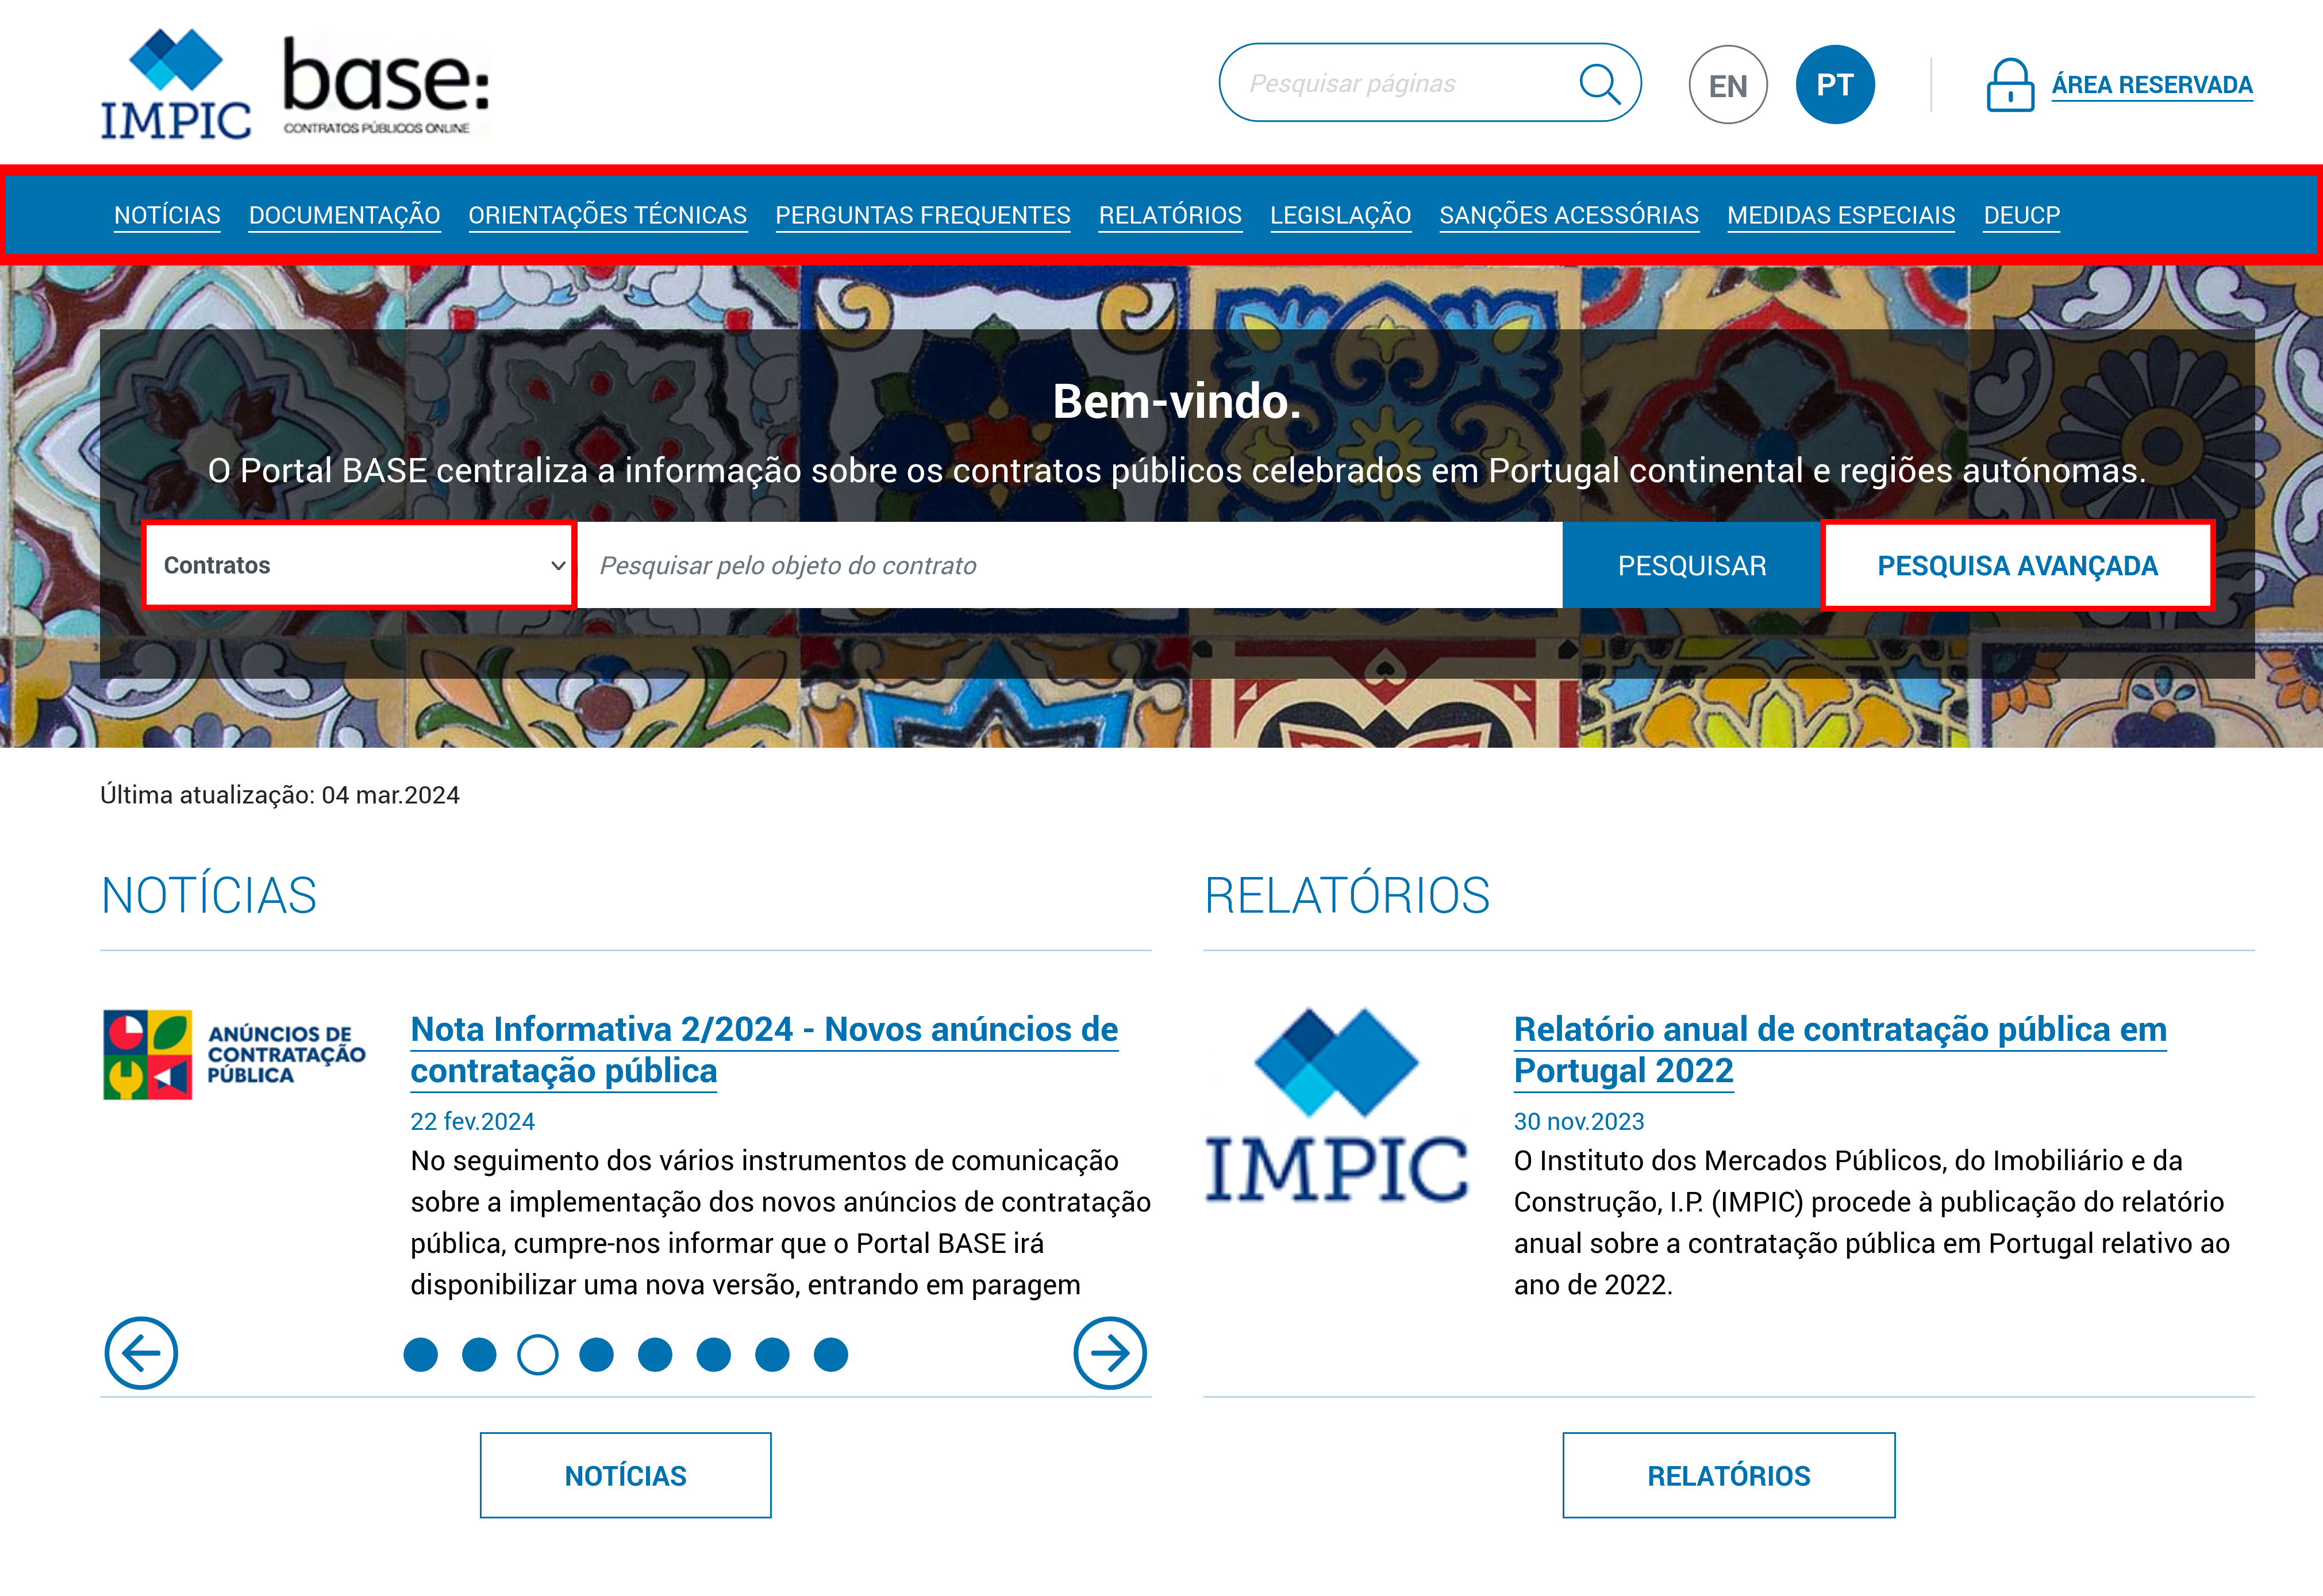
\includegraphics[width=.95\textwidth]{imagens/portalbase_init_v2.png}
	\caption{\textit{Screenshot} da página inicial do site}
	\label{fig:site1}
\end{figure}

O campo \textbf{Pesquisa Avançada} permite selecionar vários parâmetros - tipo de procedimento e contrato, intervalo de preço contratual, categoria de contrato, país/distrito/concelho - de forma a especificar a pesquisa como for desejado. 

\begin{figure}[H]
	\centering
	\includegraphics[width=.95\textwidth]{imagens/portalbase.png}
	\caption{\textit{Screenshot} do campo de pesquisa avançada do site}
	\label{fig:site2}
\end{figure}

Na figura \ref{fig:site3} encontram-se os últimos quatro contratos adicionados ao Portal BASE no momento de captura de imagem do ecrã, dia 24 de abril de 2024. De forma a aceder aos detalhes de cada um dos contratos é preciso pressionar o sinal  \img{imagens/plus.png}, que se encontra delimitado a vermelho. 

\begin{figure}[H]
	\centering
	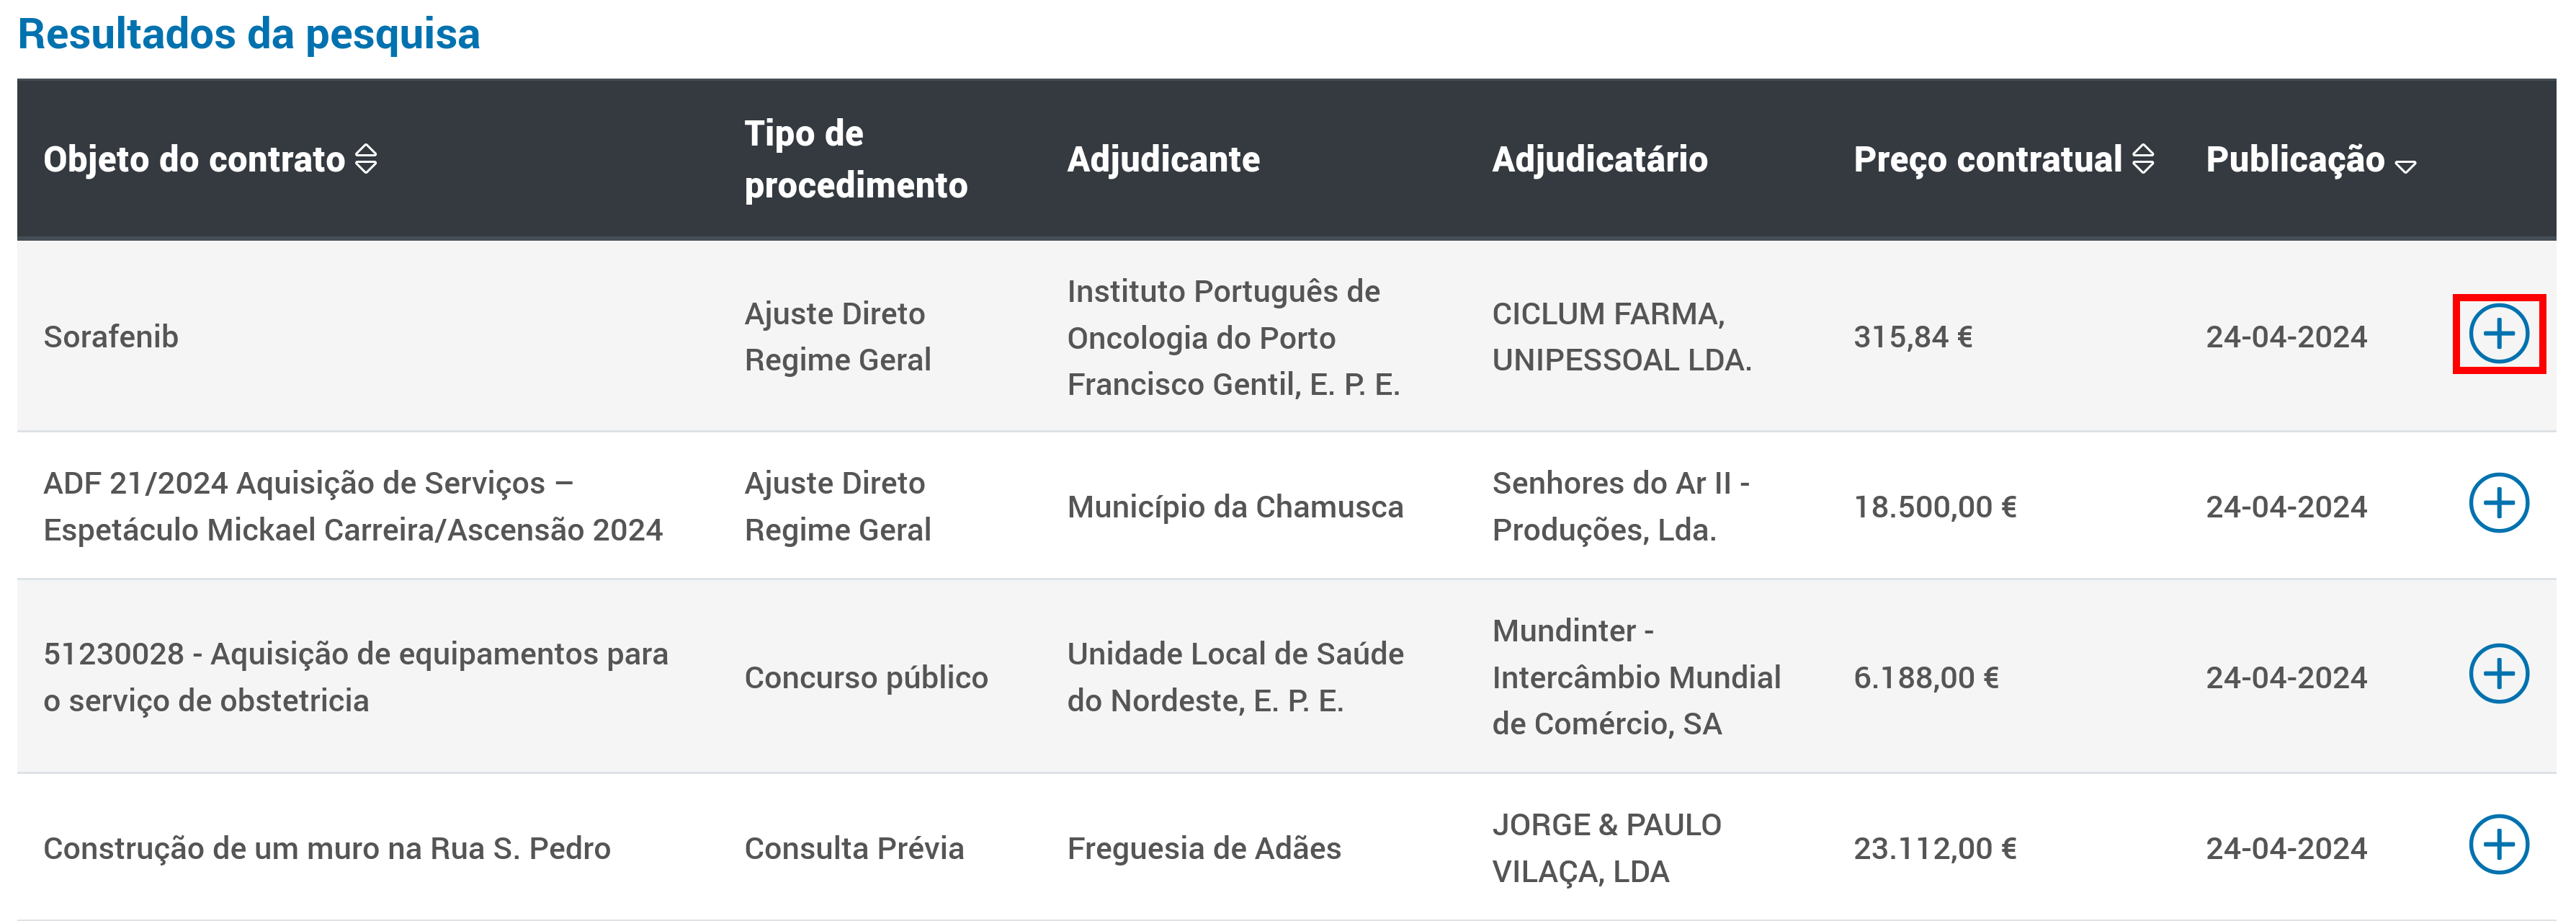
\includegraphics[width=.95\textwidth]{imagens/portalbase_pesquisa.png}
	\caption{\textit{Screenshot} de um conjunto de contratos}
	\label{fig:site3}
\end{figure}


\begin{figure}[H]
	\centering
	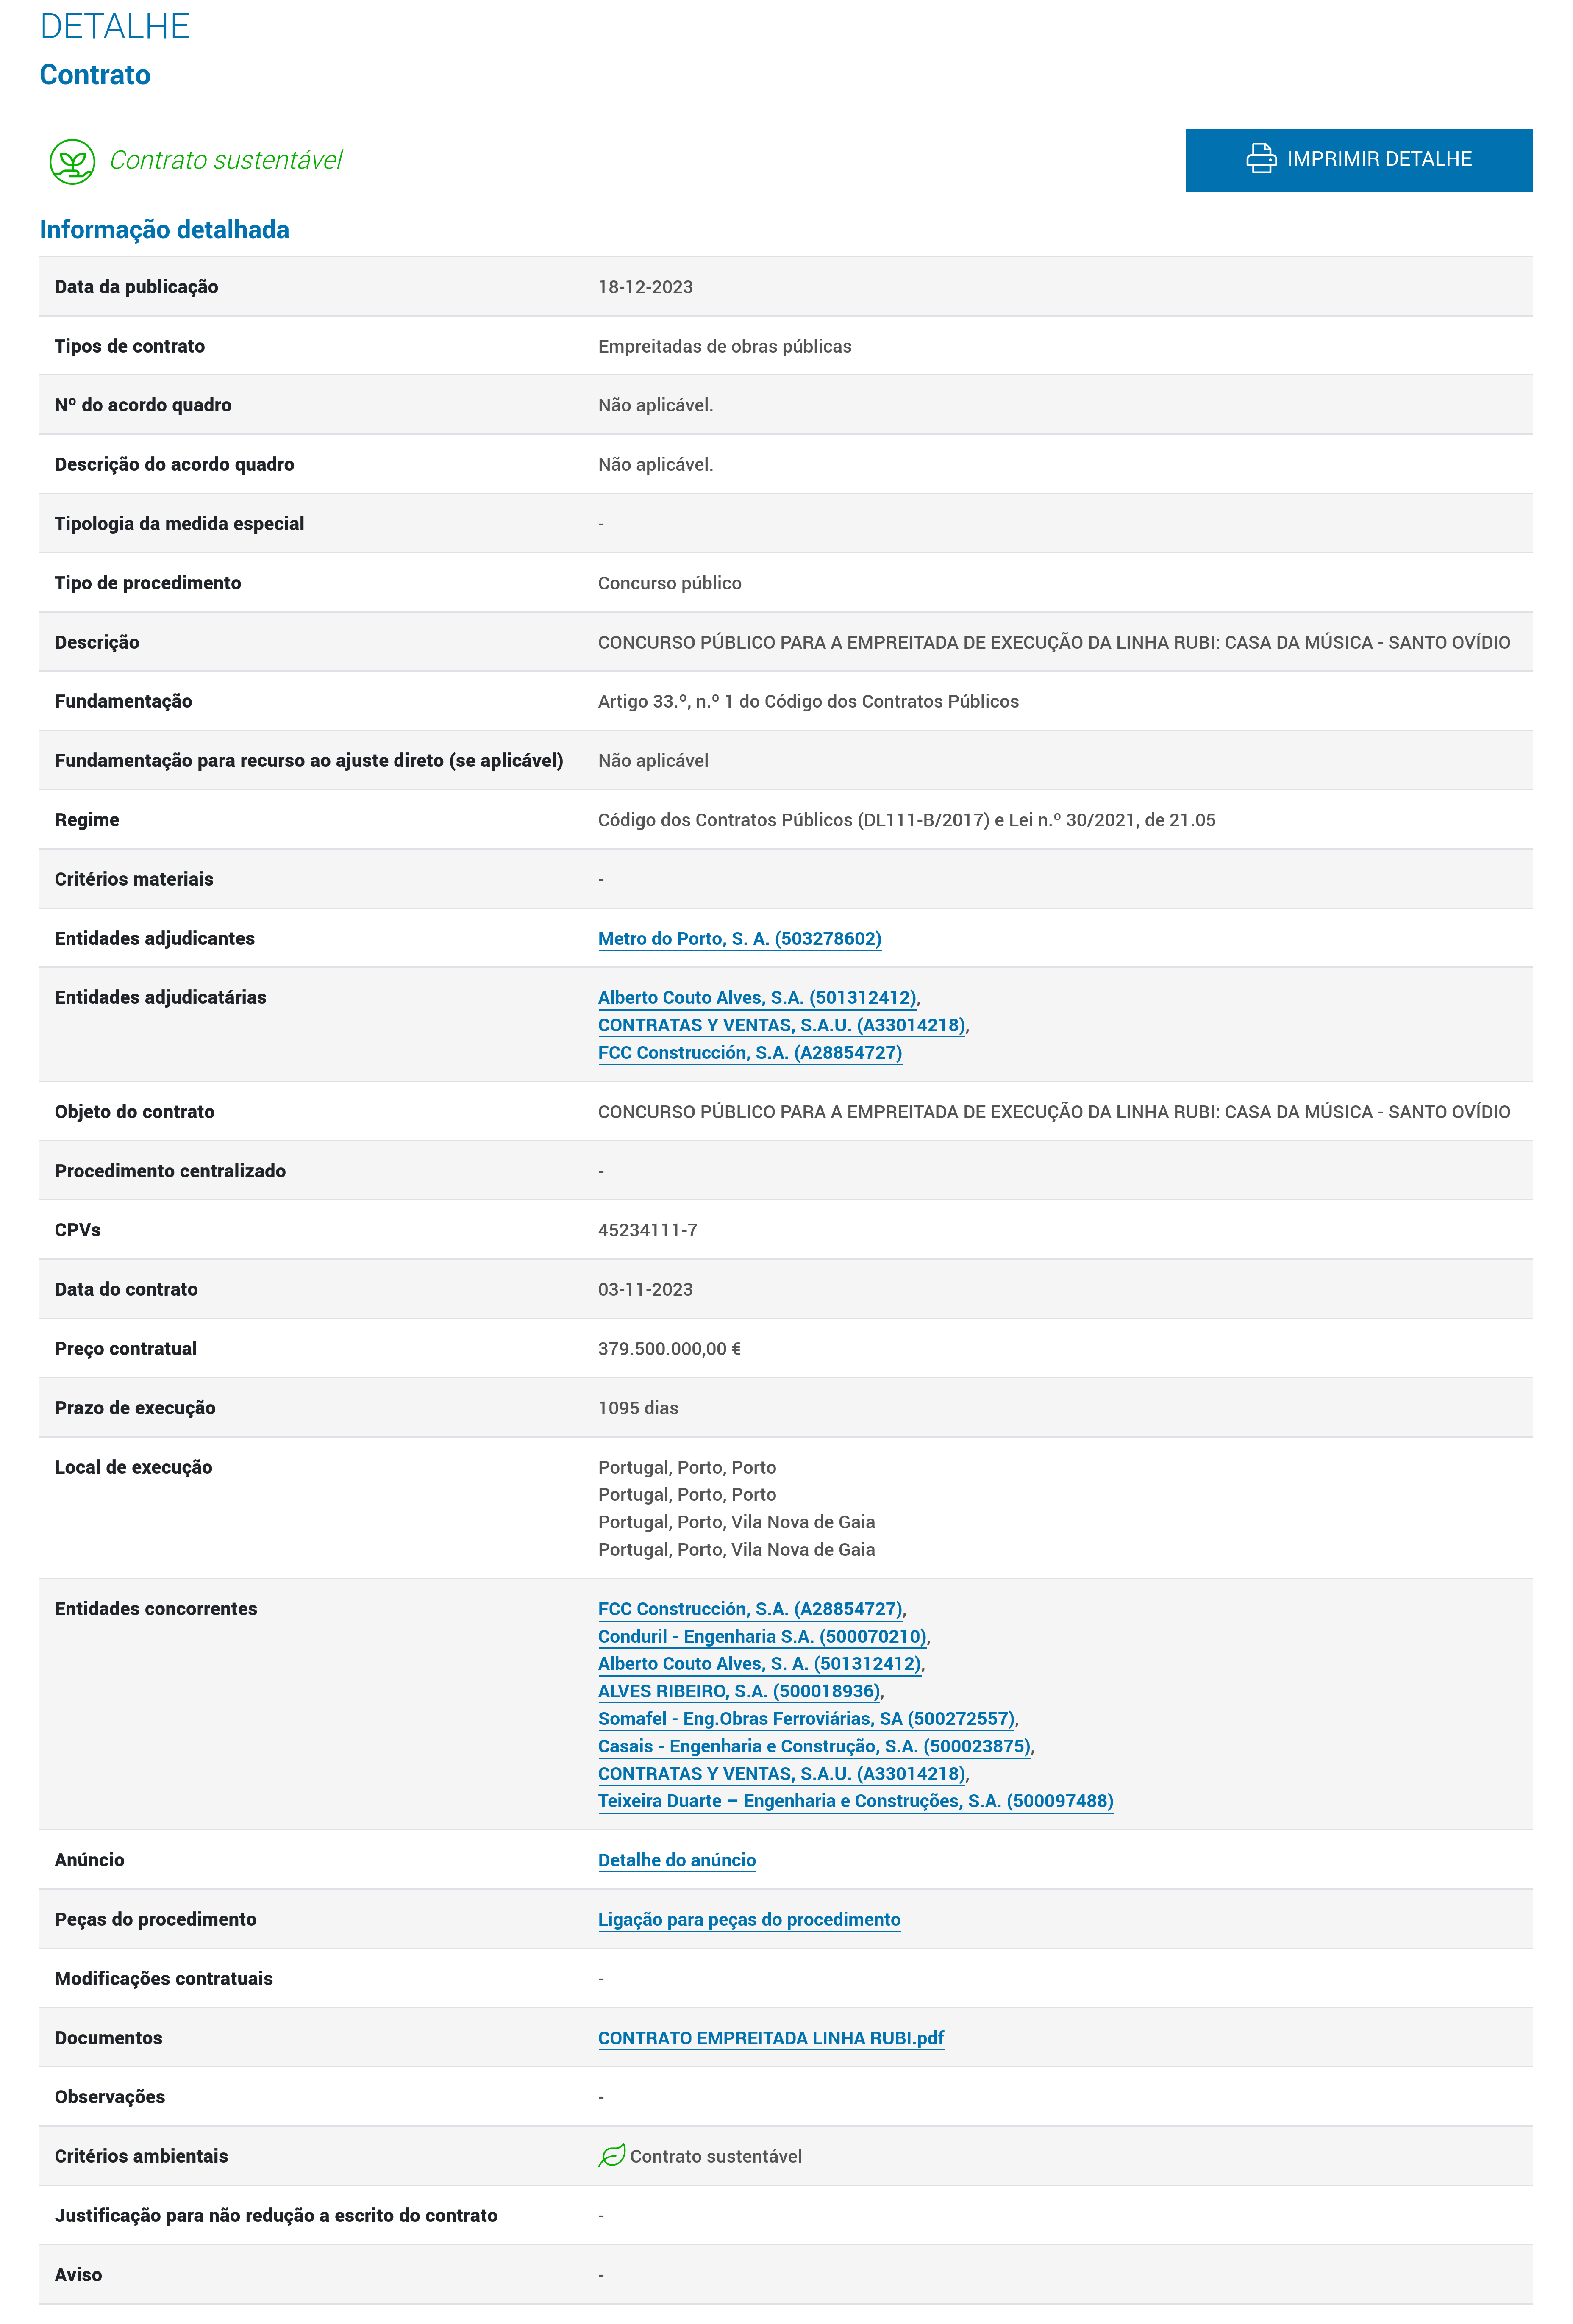
\includegraphics[width=.95\textwidth]{imagens/metro.png}
	\caption{\textit{Screenshot} dos detalhes do contrato referentes à contrução da Linha Rubi do Metro do Porto}
	\label{fig:site4}
\end{figure}

Na figura \ref{fig:site4} podem ser observados os detalhes contratuais do concurso público referente à construção da nova linha de metro do Porto.

\subsection{Entidades Envolvidas}

Existem diversas entidades que suportam o processo de contratação pública em Portugal. 

%\begin{figure}[h]
%	\centering
%	\begin{minipage}{.25\textwidth}
%		\centering
%		
\includegraphics[width=\linewidth]{imagens/ESPAP.png}
%	\end{minipage}%
%	\begin{minipage}{.25\textwidth}
%		\centering
%		
\includegraphics[scale = 0.1]{imagens/impic.jpg}
%	\end{minipage}%
%	\begin{minipage}{.25\textwidth}
%		\centering
%		
\includegraphics[width=\linewidth]{imagens/incm.png}
%	\end{minipage}%
%	\begin{minipage}{.25\textwidth}
%		\centering
%		
\includegraphics[width=.7\linewidth]{imagens/gns.png}
%	\end{minipage}
%	\caption{Entidades envolvidas no processo contratação pública}
%\end{figure}


\begin{my_enumerate}
	\item  \textbf{Instituto dos Mercados Públicos, do Imobiliário e da Construção, I.P. (IMPIC)}: É a entidade responsável por gerir o Portal BASE, monitorizar e fiscalizar as plataformas eletrónicas de contratação pública, regular os contratos públicos e é o ponto de referência com a Comissão Europeia, para efeitos do disposto no nº 5 do art.º 83 da Diretiva nº 2014/24/EU. É responsável pelo desenvolvimento de manuais de boas práticas sobre contratos públicos de aquisição de obras, de bens e de prestação de serviços. É a entidade que analisa queixas e denúncias de cidadãos e empresas.
	
	\item \textbf{Entidade de Serviços Partilhados da Administração Pública, I.P. (eSPap)}: É a entidade que desenvolve e a presta serviços no âmbito da Administração Pública. Além disso, concebe, gere e avaliar o sistema nacional de compras e assegurar a gestão do PVE, apoiando a definição de políticas estratégicas nas áreas das tecnologias de informação e comunicação (TIC) do Ministério das Finanças, garantindo o planeamento, conceção, execução e avaliação das iniciativas de informatização tecnológica dos respetivos serviços e organismos.
	
	\item \textbf{Gabinete Nacional de Segurança (GNS)}: É o organismo que garante a segurança da informação classificada no âmbito nacional e das organizações internacionais de que Portugal é parte. É responsável por crendeciar as plataformas eletrónicas de contratação pública, dos auditores de segurança, de pessoas e empresas para o acesso e manuseamento de informação classificada e entidades que atuem no âmbito do Sistema de Certificação Eletrónica do Estado - Infra-Estrutura de Chaves Públicas (SCEE).
	
	\item \textbf{Imprensa Nacional – Casa da Moeda (INCM)}: É a entidade responsável pelas publicações no Diário da República Eletrónico e no Jornal Oficial da União Europeia. Todos os anúncios dos procedimentos pré-contratuais (Concurso Público, Concurso Limitado por Prévia Qualificação, Procedimento de Negociação, Dialogo Concorrencial e Parceria para a Inovação), são publicados no Diário da República Eletrónico e, simultaneamente, são publicitados no Portal BASE (exceto nos casos de ajuste direto e consulta prévia).
	
	\item \textbf{Entidades Adjudicantes}: São estas que conduzem e decidem o procedimento de formação de contrato e são responsáveis por introduzir, no Portal, informação sobre os contratos públicos celebrados. 
	
	\item \textbf{Adjudicatário}: Titular da proposta vencedora. Tem de comprovar que respeita os requisitos exigidos para poder celebrar o contrato. A informação é enviada ao BASE pelas Plataformas Eletrónicas.
	
	\item \textbf{Plataformas Eletrónicas}: É a infraestrutura tecnológica constituída por um conjunto de aplicações, meios e serviços informáticos onde, de forma totalmente eletrónica e desmaterializada, decorre a tramitação dos procedimentos para a formação de um contrato público. 
\end{my_enumerate}







\section{Descrição da Base de Dados}



O conjunto de dados disponibilizado e utilizado ao longo deste projeto encontra-se guardado numa base de dados em PostgreSQL. Todos os dias, salvo raras exceções, são adicionados os mais recentes contratos celebrados ao Portal BASE. Por sua vez, todos os dias são adicionados à base de dados todos os novos contratos adicionados ao Portal BASE do dia anterior, havendo um desfasamento de 1 dia de forma a garantir que todos os contratos são coletados. 


\begin{figure}[H]
	\centering
	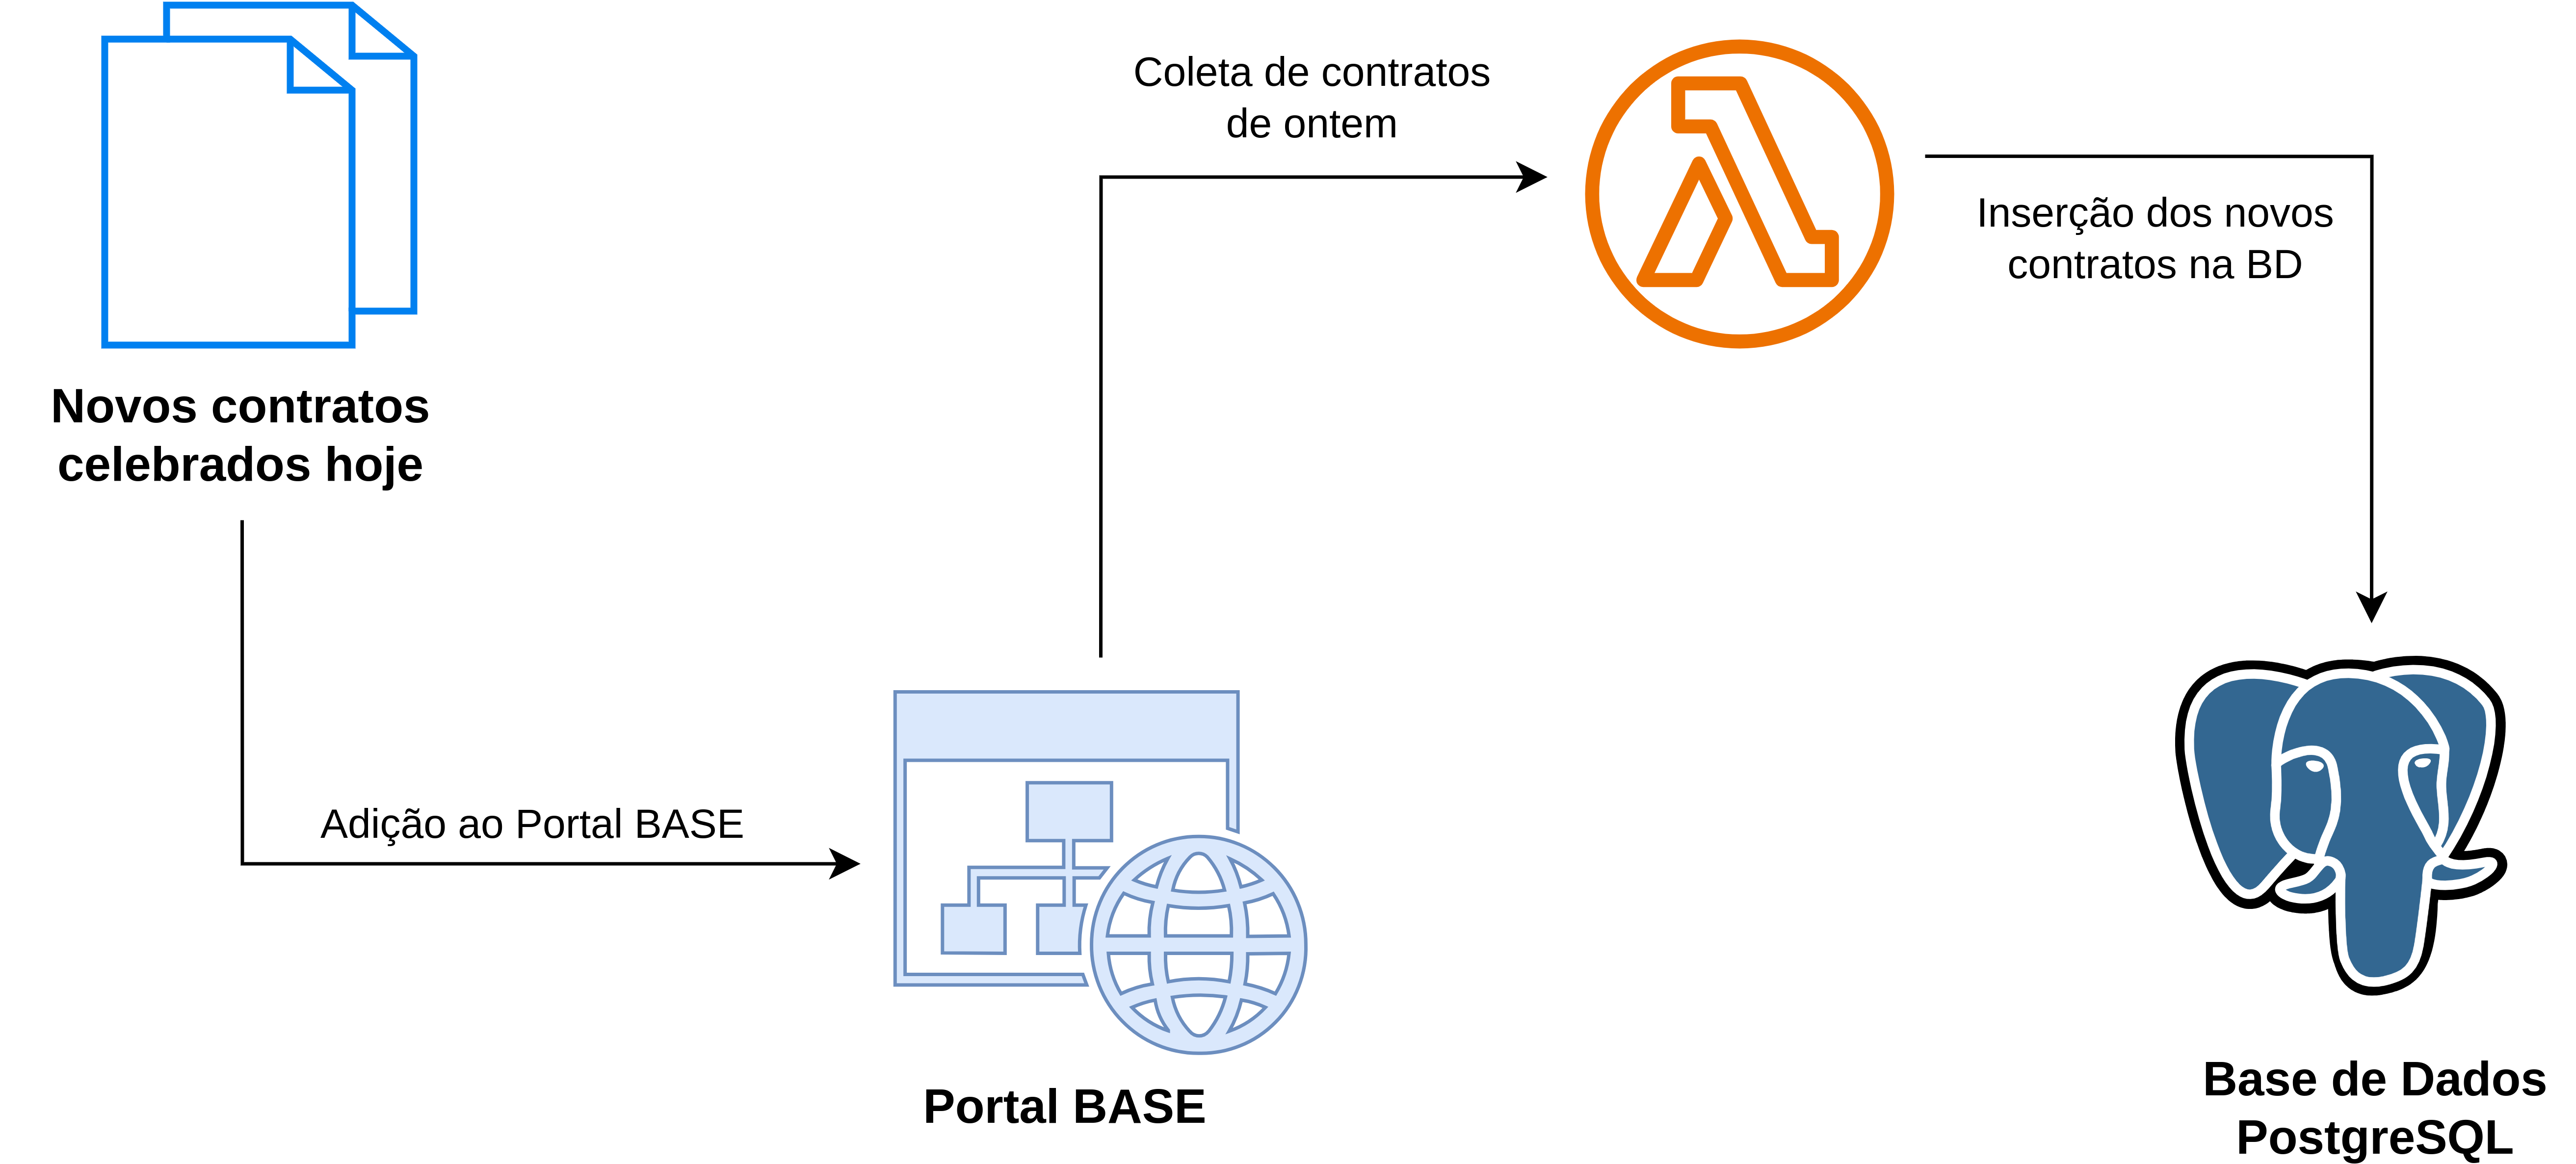
\includegraphics[width=0.7\textwidth]{imagens/portal_coleta.png}
	\caption{Processo de coleta de contratos e contrução da base de dados}
	\label{fig:processocoleta}
\end{figure}


Até ao primeiro dia do mês de abril do presente ano civil, o conjunto de dados conta com 1054929 contratos públicos, celebrados desde o dia 13 de maio 2003. 

De todas as colunas, as que reveleram maior utilidade foram as seguintes : 


\begin{my_itemize}
	
\item \textbf{id} (integer): É o número que permite identificar um contrato específico no conjunto total de contratos. Cada contrato tem um identificador único.

\item \textbf{n\_anuncio} (text): O número de anúncio é o número que permite identificar o anúncio referente a um determinado procedimento de contratação pública.


\item \textbf{anuncio\_preco\_base} (float): O preço base é definido como o preço máximo que a entidade adjudicante está disposta a pagar pela execução de todas as prestações que constituem o objeto do contrato a celebrar.

\item \textbf{anuncio\_proposalDeadline} (date): Este campo diz respeito ao número de dias em que é possível submeter uma proposta a um determinado procedimento por parte de uma entidade concorrente. 

\item \textbf{tipo\_procedimento} (text): Este parâmetro permite identificar o tipo de procedimento, de acordo com aqueles enunciados na tabela \ref{table:2}, de um  determinado contrato público.

\item \textbf{objeto\_contrato} (text): O objeto de contrato consiste numa descrição mais detalhada do tipo de objeto celebrado. 

\item \textbf{data\_publicacao} (date): A data de publicação diz respeito à data de publicação do contrato na plataforma Portal BASE.

\item \textbf{data\_celebracao} (date): A data de celebração diz respeito à data de celebração do contrato. 

\item \textbf{preco\_contratual} (float): O  preço contratual é o preço a pagar pela entidade adjudicante à entidade vencedora após celebração do objeto contratual. 

\item \textbf{entidade\_adjudicante} (text): Este campo contém o nome, número de identificação fiscal e URL que remete para a página \textit{web} do Portal BASE com todos os contratos celebrados de uma determinada entidade adjudicante. 

\begin{figure}[H]
	\centering
	
\includegraphics[width=.9\textwidth]{imagens/adjudicante.png}
	\caption{Exemplo de uma entidade adjudicante da base de dados}
	\label{fig:adjudicante}
\end{figure}

\item \textbf{fundamentacao} (text): A fundamentação diz respeito ao artigo do CCP utilizado para justificar a adoção do procedimento escolhido. 

\item \textbf{entidades\_contratadas} (text): À semelhança do campo \textbf{entidade\_adjudicante}, este campo contém o nome, número de identificação fiscal e URL que remete para a página \textit{web} do Portal BASE com todos os contratos celebrados de uma determinada entidade adjudicatária. 

\item \textbf{entidades\_concorrentes} (text): Neste campo é possível encontrar o nome, número de identificação fiscal e URL que remete para a página \textit{web} do Portal BASE com todos os contratos celebrados para todas as entidades que concorrem a um determinado contrato público. Quando existe mais do que uma entidade concorrente, a separação entre entidades é feita através do caracter \(|||\).



\begin{figure}[H]
	\centering
	
\includegraphics[width=.9\textwidth]{imagens/concorrentes.png}
	\caption{Exemplo de entidades concorrentes da base de dados}
	\label{fig:concorrentes}
\end{figure}


\item \textbf{url\_anuncio} (text): Contém um \textit{link} que redireciona para a página \textit{web} que contém os detalhes do anúncio.

\item \textbf{cpv} (text): Contém o CPV do contrato. CPV é a sigla de \textit{Common Procurement Vocabulary}. O CPV é um código de 8 dígitos, usado no processo de contratação, que permite especificar e categorizar de forma hierárquica serviços e produtos. 

\begin{my_itemize}
	\item[$\circ$]  Os 2 primeiros dígitos permitem identificar a \textbf{divisão} do serviço/produto. No total, existem 45 divisões.
	\item[$\circ$]  Os 3 primeiros dígitos permitem identificar o \textbf{grupo}. No total, existem 272 grupos.
	\item[$\circ$]  Os 4 primeiros dígitos permitem identificar a \textbf{classe}. No total, existem, 1002 classes.
	\item[$\circ$]  Os 5 primeiros dígitos permitem identificar a \textbf{categoria}. No total, existem 2379 categorias.
	\item[$\circ$]  Os 6 primeiros dígitos permitem identificar a \textbf{subcategoria}. No total, existem 5756 subcategorias.
\end{my_itemize}

Atente-se no seguinte caso, a título de exemplo:

\begin{figure}[H]
	\centering
	
\includegraphics[width=0.7\textwidth]{imagens/cpv.png}
	\caption{CPV de um contrato referente a veículos de combate de incêndios.}
	\label{fig:cpv}
\end{figure}


\begin{my_itemize}
	\item[$\circ$]  \textbf{Divisão:} 34 - Equipamentos de transporte e produtos auxiliares ao transporte
	\item[$\circ$]  \textbf{Grupo:} 341 - Veículos motorizados
	\item[$\circ$]  \textbf{Classe:} 3414 - Veículos motorizados pesados
	\item[$\circ$]  \textbf{Categoria:} 34144 - Veículos motorizados para fins especiais
	\item[$\circ$]  \textbf{Subcategoria:} 34144210 - Veículos de combate a incêndio
\end{my_itemize}



\item \textbf{contractType} (text): Este campo diz respeito aos tipos de contrato apresentados na tabela \ref{table:3}. 

\item \textbf{executionPlace} (text): Indica o local de execução do contrato. 

\item \textbf{totalEffectivePrice} (float): Na eventualidade de existirem alterações do preço contratual após a celebração do contrato, este campo é preenchido. Existem, também, casos em que o preço contratual diz respeito à unidade em questão (p. ex. quilómetro, hora). Nessa situação, o preço total efetivo é o preço total após prestação do serviço \cite{jardinagem}.  

\end{my_itemize}

De entre o universo de contratos celebrados, pode-se atentar na Tabela \ref{tab:contratos} como estes se distribuem consoante os diferentes tipos de procedimento.

\begin{table}[H]
	\centering
	\renewcommand{\arraystretch}{1.15}
	\setlength{\tabcolsep}{15pt}
	\resizebox{\textwidth}{!}} \\ \hline
			Ajuste Direto Regime Geral                                                     & 530462                                                                   & 50.3                                                            \\ \hline
			\rowcolor[HTML]{EFEFEF} 
			Consulta Prévia                                                                & 223037                                                                   & 21.1                                                            \\ \hline
			Concurso público                                                               & 125996                                                                   & 11.9                                                            \\ \hline
			\rowcolor[HTML]{EFEFEF} 
			Ao abrigo de acordo-quadro (art.º 259.º)                                       & 109346                                                                   & 10.4                                                            \\ \hline
			Ajuste direto simplificado                                                     & 38345                                                                    & 3.6                                                             \\ \hline
			\rowcolor[HTML]{EFEFEF} 
			Ao abrigo de acordo-quadro (art.º 258.º)                                       & 23941                                                                    & 2.3                                                             \\ \hline
			Concurso limitado por prévia qualificação                                      & 1909                                                                     & $< 1$                                                            \\ \hline
			\rowcolor[HTML]{EFEFEF} 
			Ajuste direto simplificado ao abrigo da Lei n.º 30/2021, de 21.05              & 1171                                                                     & $< 1$                                                           \\ \hline
			Consulta Prévia Simplificada                                                   & 922                                                                      & $< 1$                                                            \\ \hline
			\rowcolor[HTML]{EFEFEF} 
			Contratação excluída II                                                        & 202                                                                      & $< 1$                                                            \\ \hline
			Setores especiais – isenção parte II                                           & 150                                                                      & $< 1$                                                          \\ \hline
			\rowcolor[HTML]{EFEFEF} 
			Procedimento de negociação                                                     & 43                                                                       & $< 1$                                                          \\ \hline
			Concurso público simplificado                                                  & 41                                                                       & $< 1$                                                          \\ \hline
			\rowcolor[HTML]{EFEFEF} 
			Consulta prévia ao abrigo do artigo 7º da Lei n.º 30/2021, de 21.05            & 23                                                                       & $< 1$                                                          \\ \hline
			Ajuste Direto Regime Geral ao abrigo do artigo 7º da Lei n.º 30/2021, de 21.05 & 16                                                                       & $< 1$                                                          \\ \hline
			\rowcolor[HTML]{EFEFEF} 
			Serviços sociais e outros serviços específicos                                 & 9                                                                        & $< 1$                                                          \\ \hline
			Concurso de conceção simplificado                                              & 4                                                                        & $< 1$                                                          \\ \hline
			\rowcolor[HTML]{EFEFEF} 
			Parceria para a inovação                                                       & 2                                                                        & $< 1$                                                          \\ \hline
			Concurso de ideias simplificado                                                & 1                                                                        & $< 1$                                                          \\ \hline
			\rowcolor[HTML]{EFEFEF} 
			Não especificado & 1                                                                        & $< 1$                                                           \\ \hline
		\end{tabular}%
	}
	\caption{Número de contratos públicos e repetiva fração para os vários tipos de procedimento}
	\label{tab:contratos}	
\end{table}

Como se pode observar na Tabela \ref{tab:contratos}, os tipos de procedimento com maior relevo são o Ajuste Direto em Regime Geral, a Consulta Prévia, o Concurso Público e contratos ao abrigo de acordo-quadro, com especial ênfase no primeiro que perfaz 50\% dos contratos. 


\begin{figure}[H]
	\centering
	\begin{minipage}{.49\linewidth}
		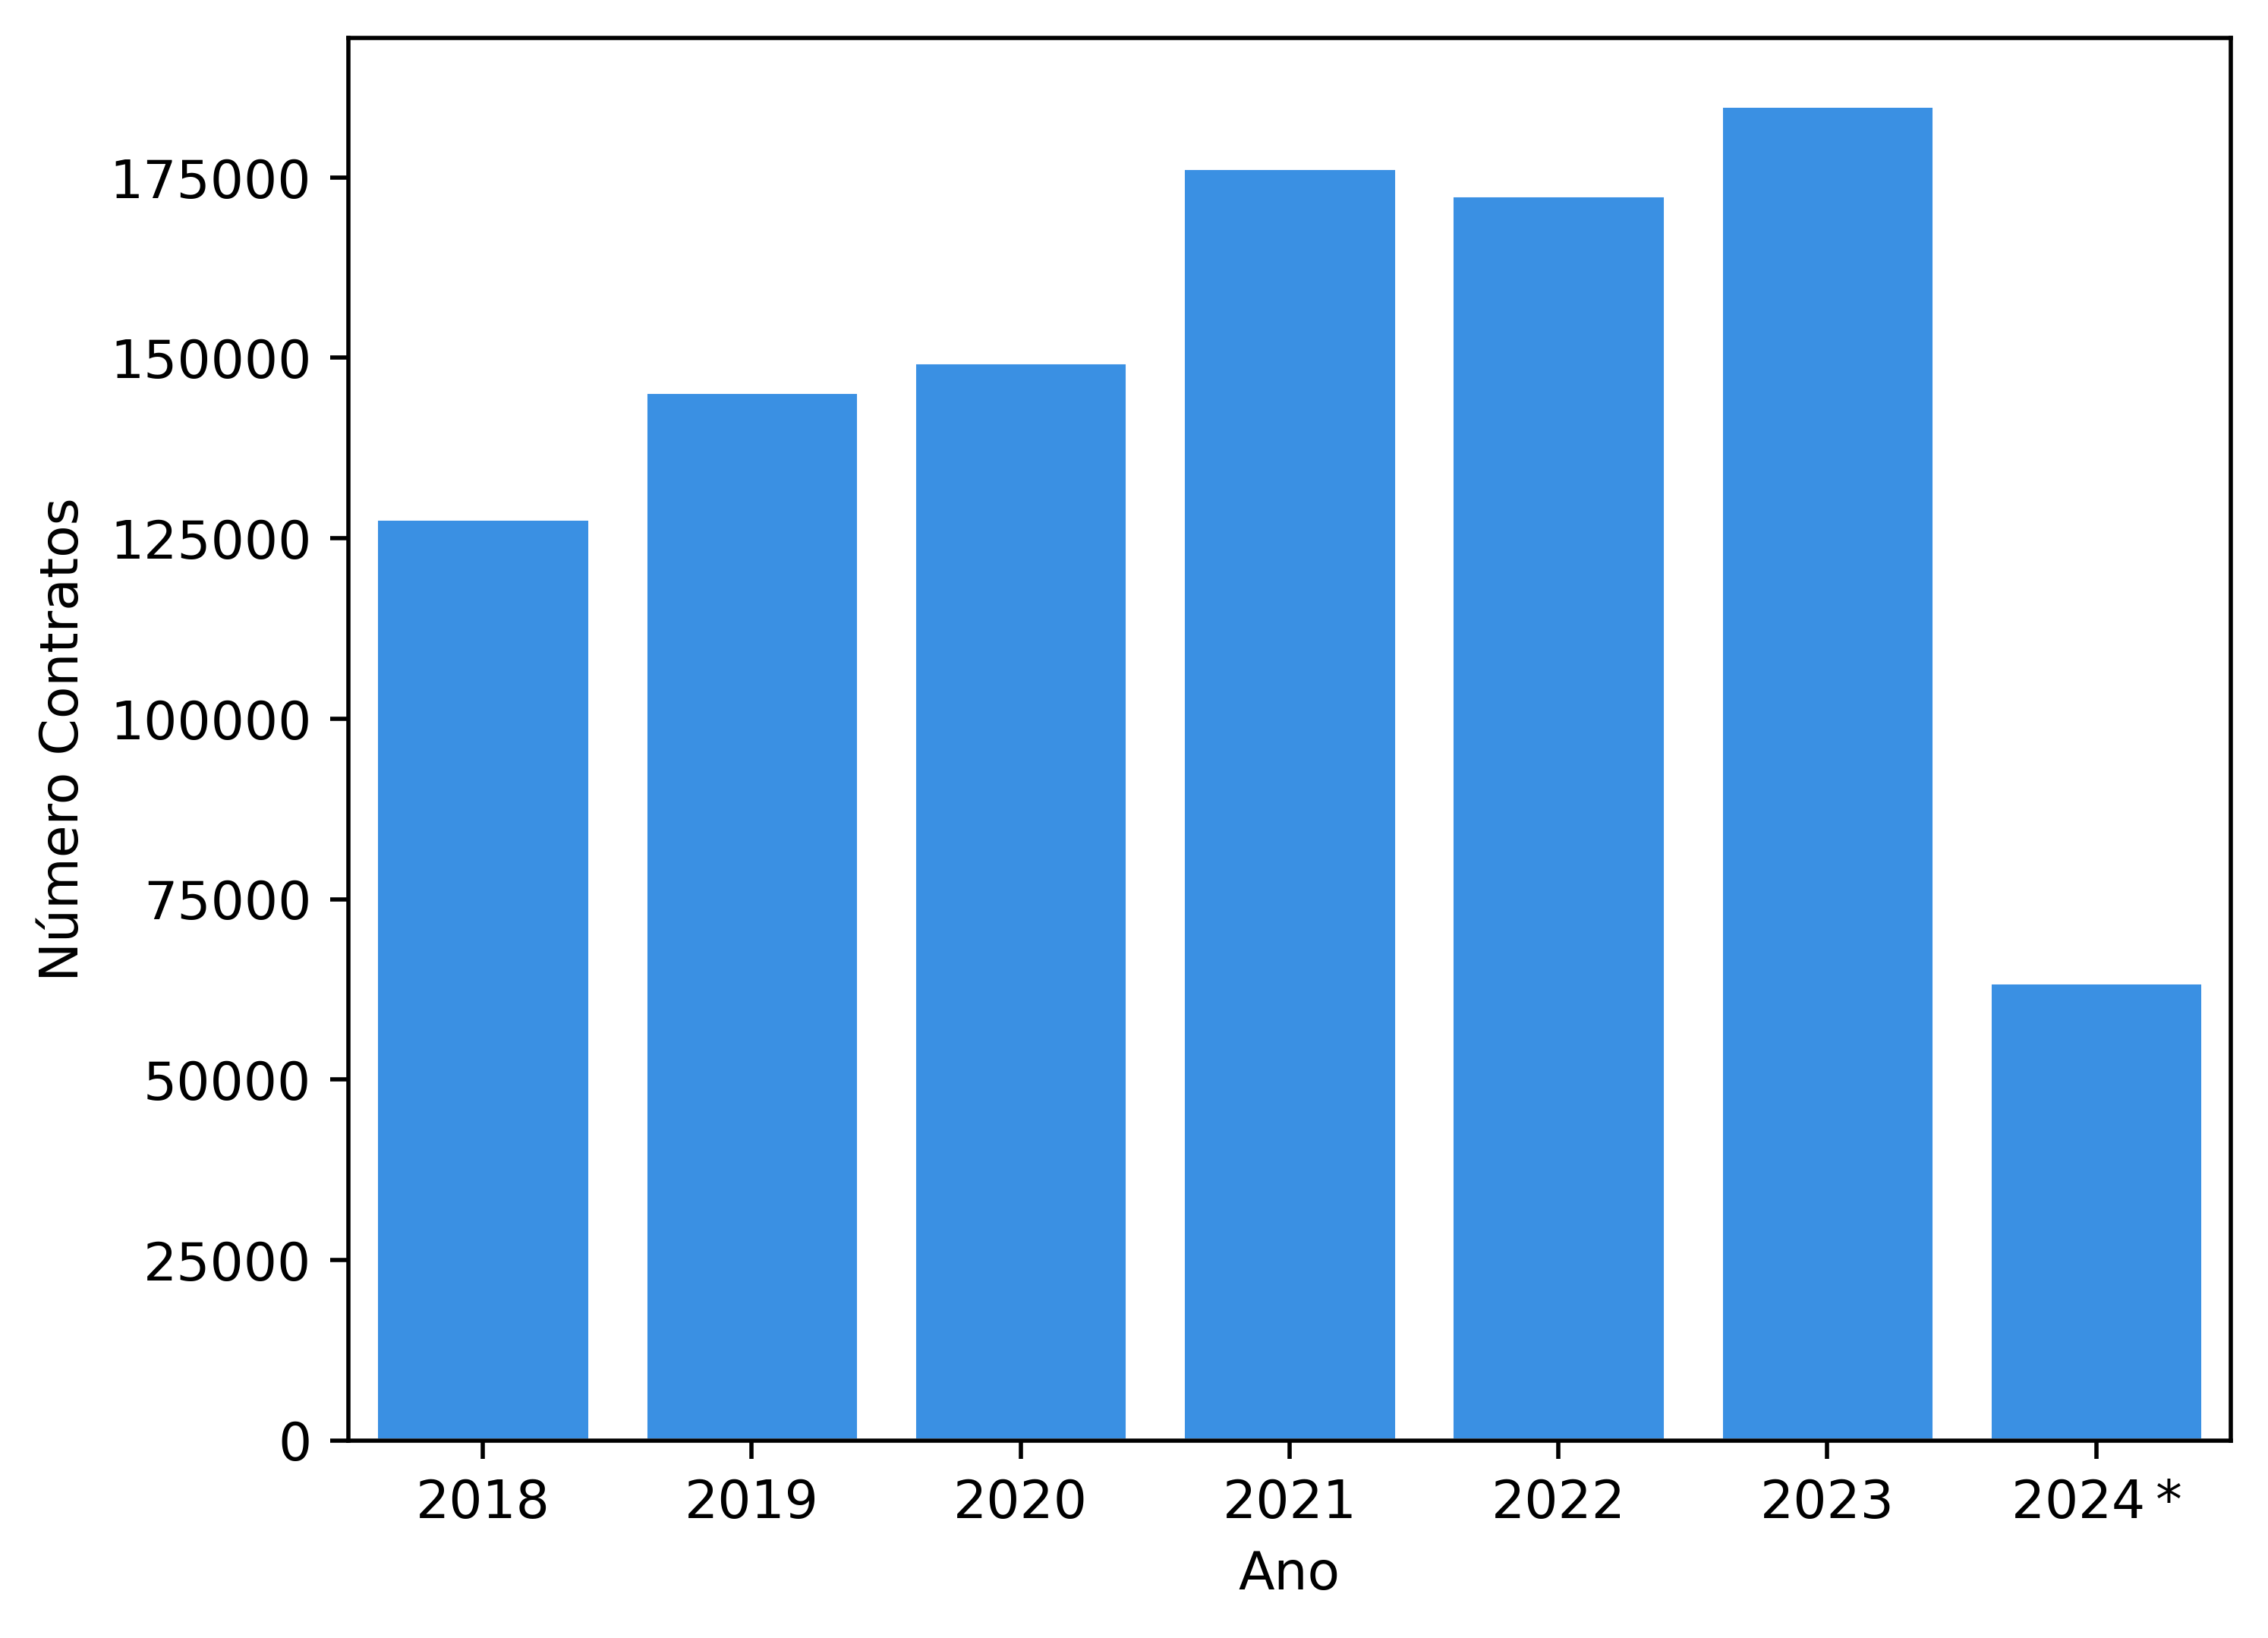
\includegraphics[width=\linewidth]{imagens/contratos_ano.png}
		\caption{Número de contratos celebrados por ano, entre 2018 e 2024, para todas as tipologias}
		\label{fig:numcontrs}
	\end{minipage}
	\hfill
	\begin{minipage}{.49\linewidth}
		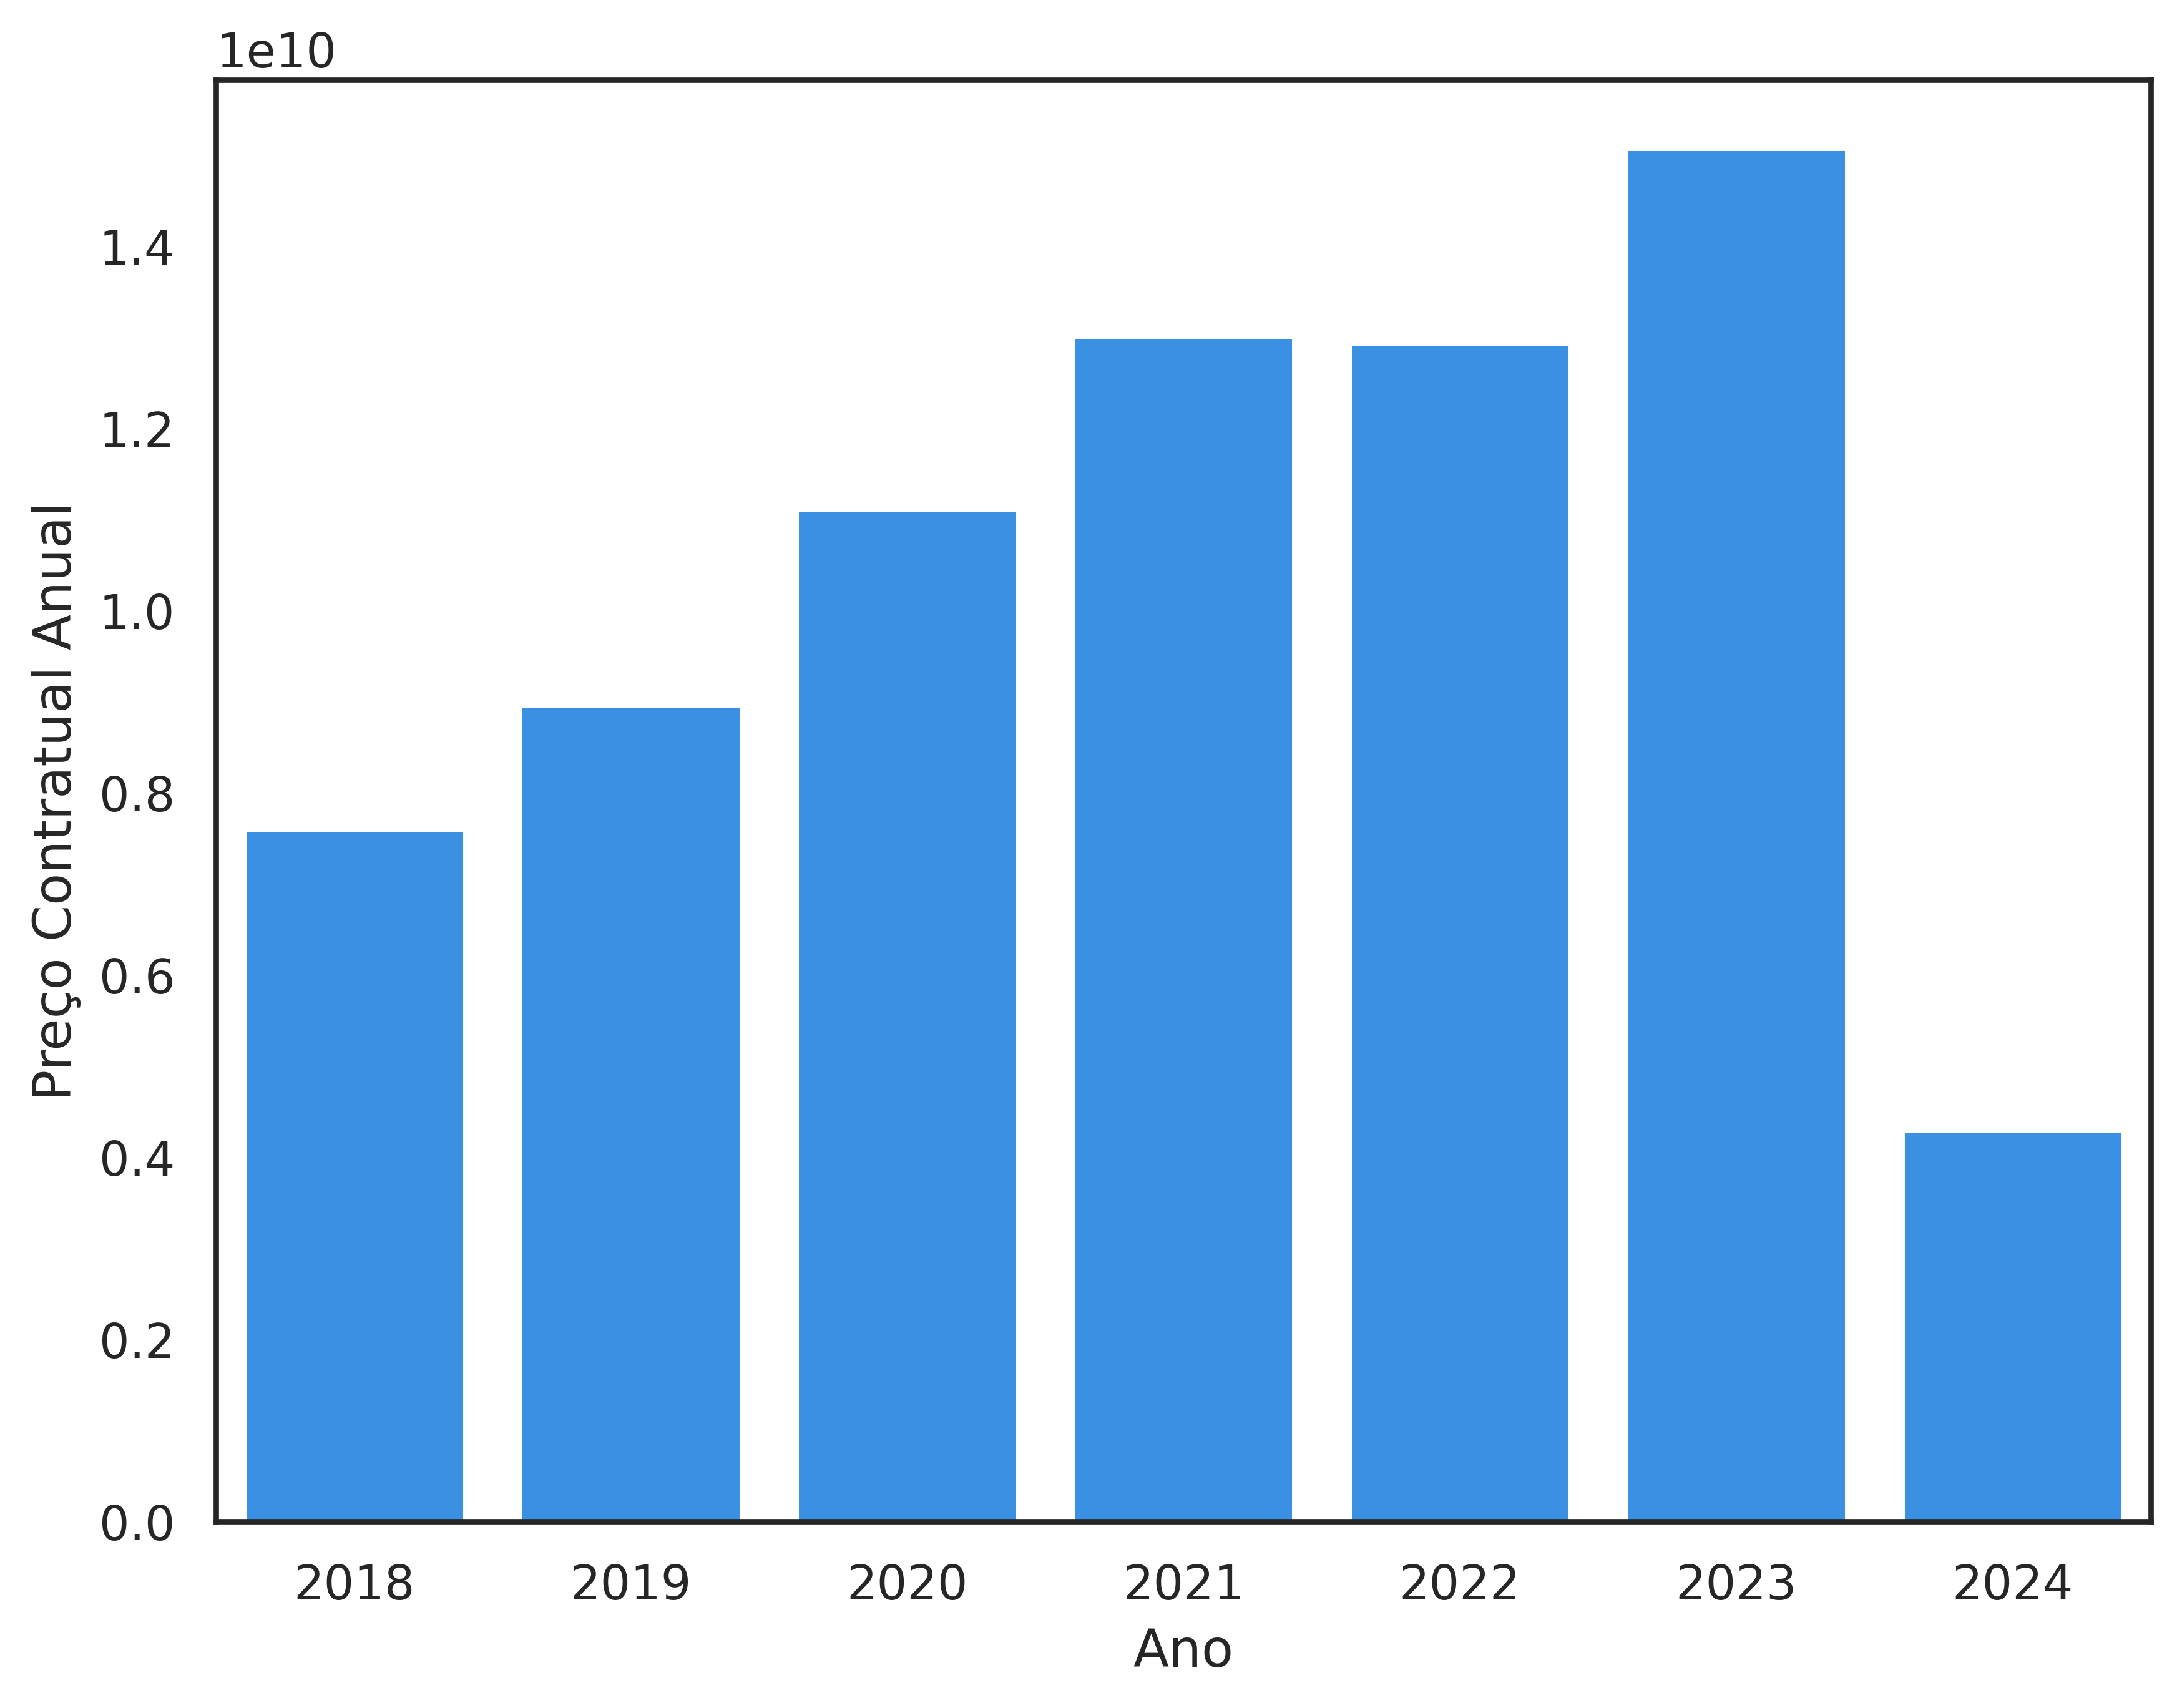
\includegraphics[width=\linewidth]{imagens/precocontr_ano.png}
		\caption{Preço contratual total por ano, entre 2018 e 2024, para todas as tipologias}
		\label{fig:precoscontrs}
	\end{minipage}
\end{figure}


%\begin{wrapfigure}{R}{0.45\textwidth}
%	\centering
%	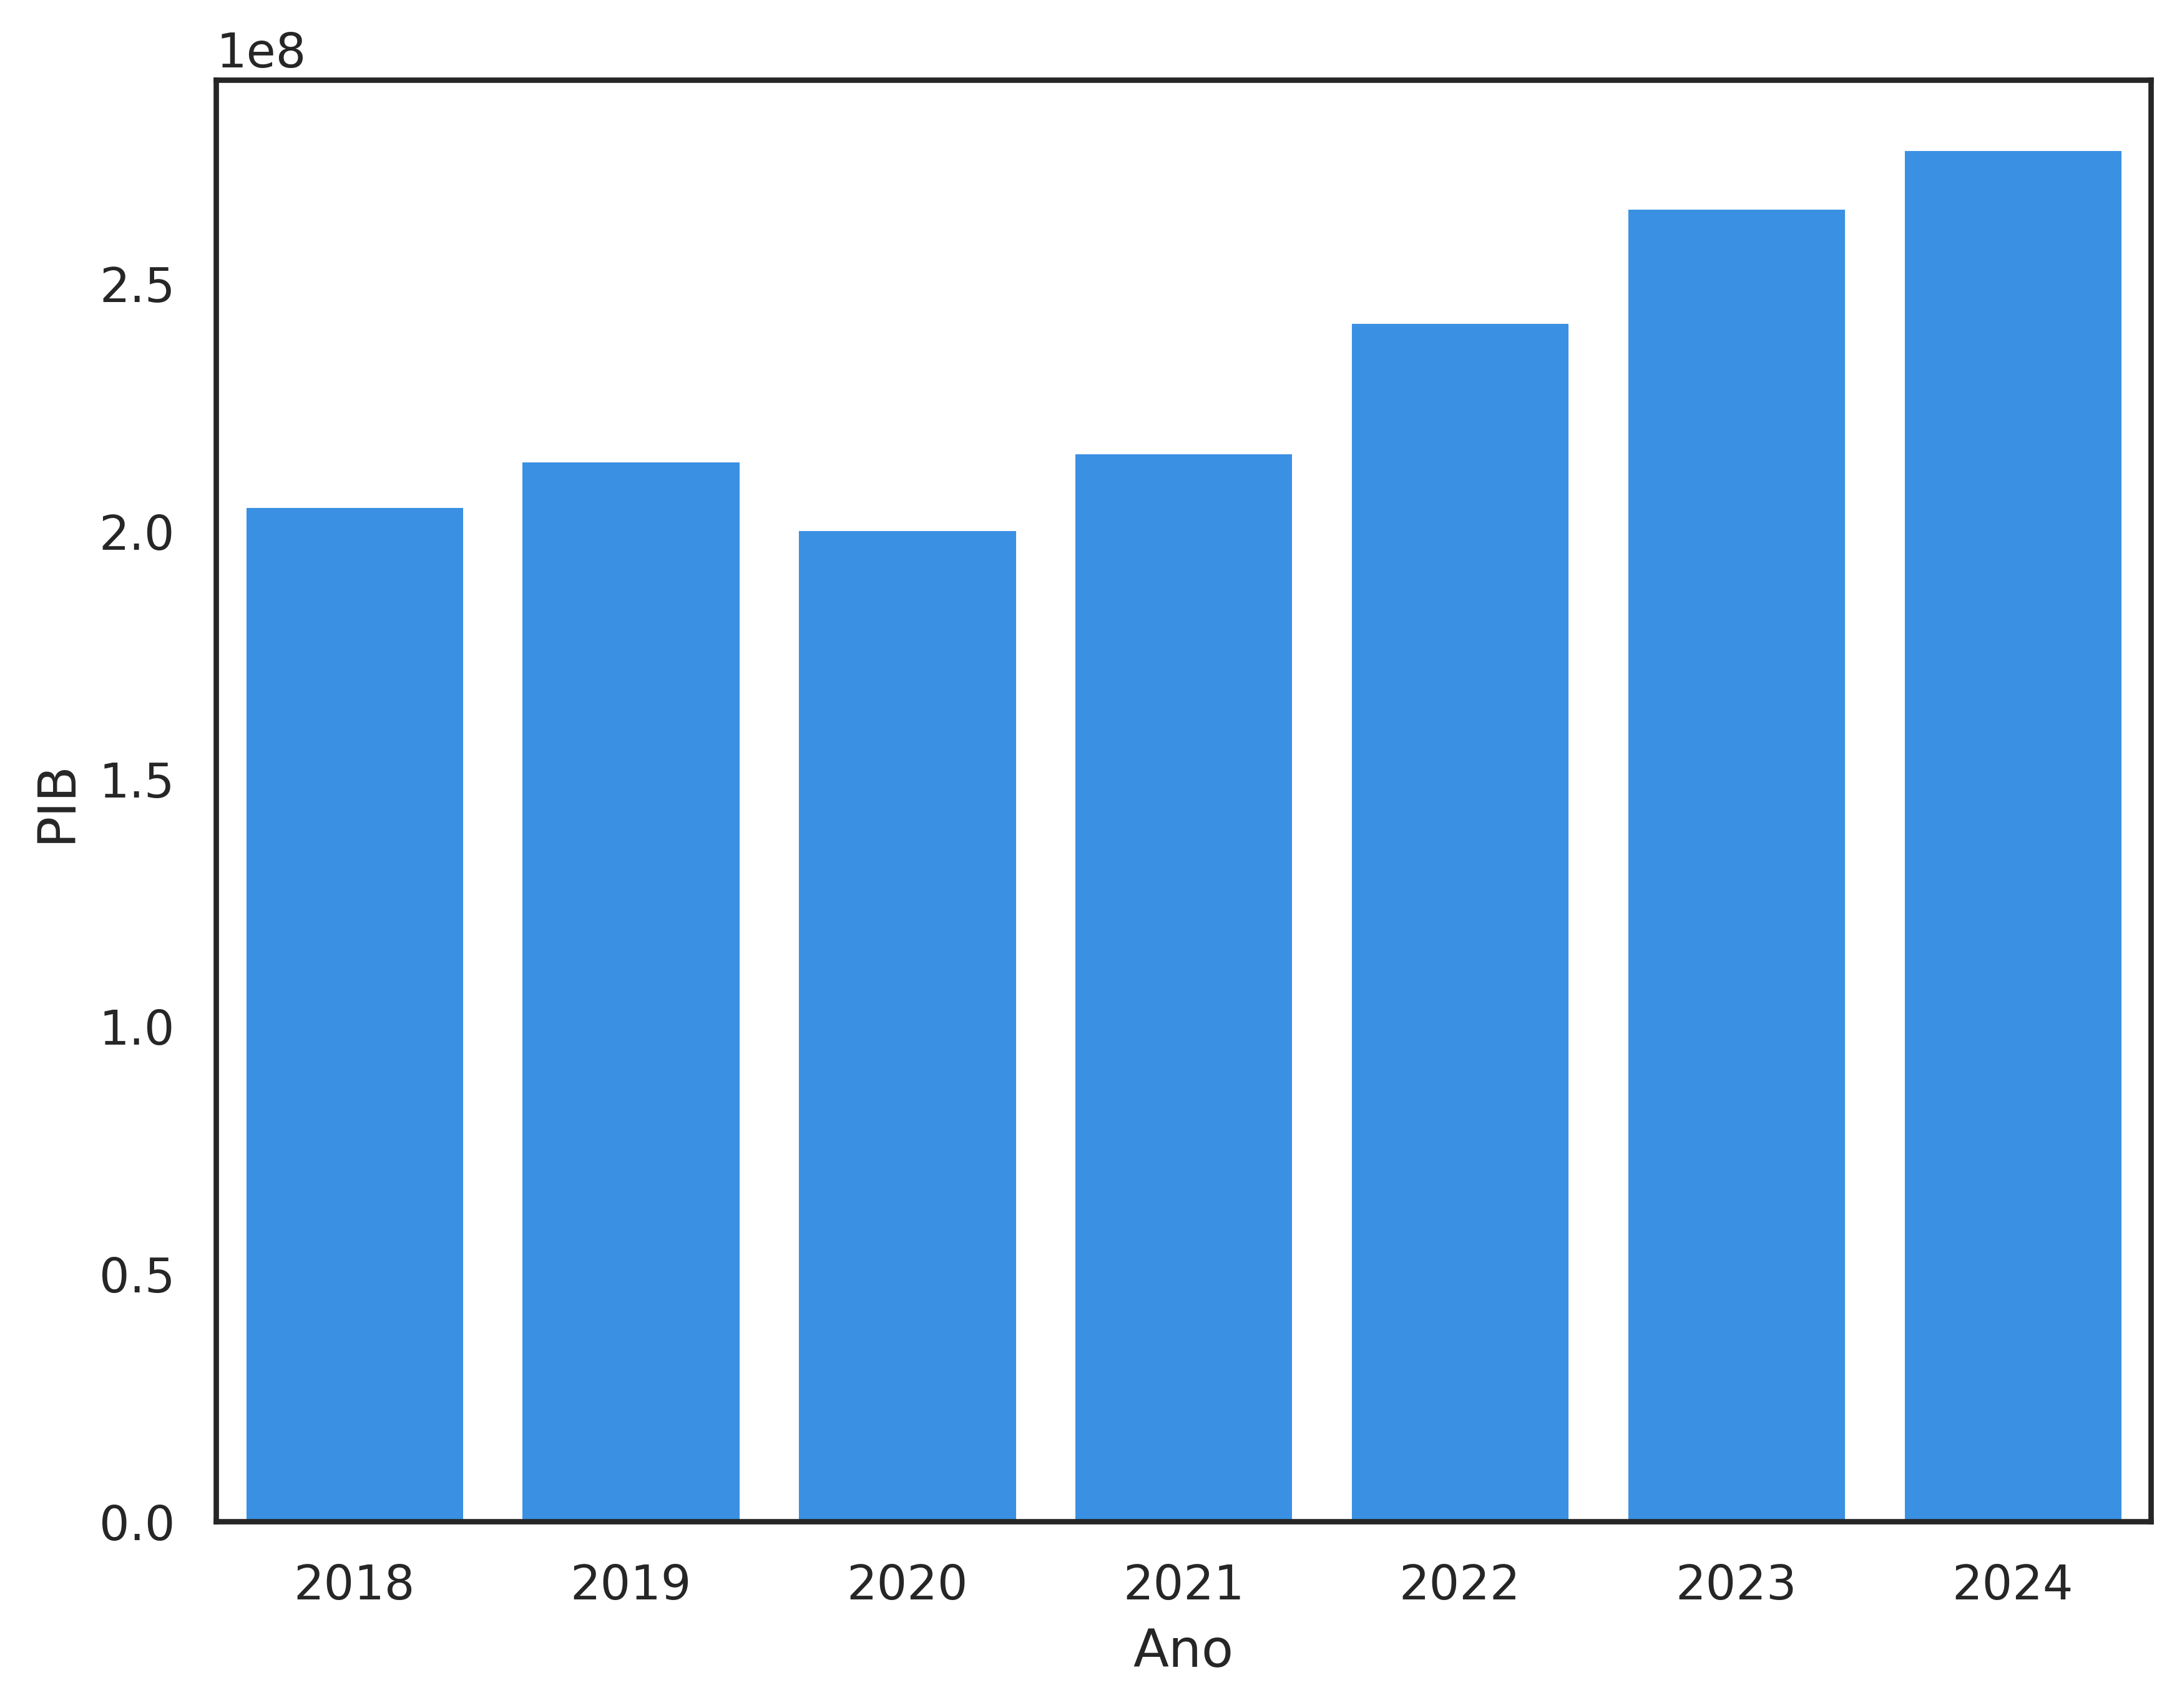
\includegraphics[width=0.45\textwidth]{imagens/pib.png}
%	\caption{PIB português entre 2018 e 2024}
%\end{wrapfigure}


Verifica-se,a partir das Figuras \ref{fig:numcontrs} e \ref{fig:precoscontrs}, uma tendência crescente do número de contratos celebrados entre 2018 e 2023, sendo esta tendência acompanhada, igualmente, por um crescimento do preço contratual total por ano, respetivamente. A partir da Figura \ref{fig:distritos}, pode ser constatado que existe uma prevalência de contratos celebrados nos distritos de Lisboa e do Porto, de forma oposta aos distritos do interior. Existe, também, um elevado de número de contratos cujo distrito é identificado como \textit{Outro}. Estes casos dizem respeito a erros de preenchimentos aquando da colocação dos contratos no Portal BASE. No campo \textbf{executionPlace} destes contratos verificava-se um dos três cenários: o campo encontrava-se vazio, era inserido \textit{Distrito não determinado} ou era inserido \textit{Portugal Continental}. 
A partir da Figura \ref{fig:cpvs}, observa-se que existe uma predominância de contratos públicos cuja divisão do CPV - os dois primeiros dígitos deste identificador - começa por 33. Esta divisão diz respeito a contratos que envolvam a aquisição de equipamento médico, medicamentos e produtos para cuidados pessoais. 



\begin{table}[H]
	\centering
	\renewcommand{\arraystretch}{1.35}
	\setlength{\tabcolsep}{20pt}
	\resizebox{\textwidth}{!}{%
		\begin{tabular}{l|l}
			\textbf{33} & {\color[HTML]{000000} Equipamento médico, medicamentos, e produtos para cuidados pessoais}     \\
			\textbf{45} & Construção                                                                                     \\
			\textbf{79} & Serviços a empresas: direto, comercialização, consultoria, recrutamento, impressão e segurança \\
			\textbf{50} & Serviços de reparação e manuntenção                                                           
		\end{tabular}%
	}
	\caption{Descrição das principais divisões de CPV}
	\label{tab:maincpvs}
\end{table}


%\begin{table}[H]
%	\centering
%	\renewcommand{\arraystretch}{1.15}
%	\setlength{\tabcolsep}{15pt}
%	\resizebox{\textwidth}{!}{%
%		\begin{tabular}{ccccccccc}
%			\hline
%			\rowcolor[HTML]{C0C0C0} 
%			\textbf{Ano} & \textbf{Count} & \textbf{Média} & \textbf{D.Padrão} & \textbf{Min} & \textbf{Q1} & \textbf{Q2} & \textbf{Q3} & \textbf{Máx} \\ \hline
%			2024         & 90658          & 77953.18       & 1669717           & 0            & 3000        & 10800       & 29960.68    & 321888000    \\ \hline
%			\rowcolor[HTML]{EFEFEF} 
%			2023         & 191800         & 80514.25       & 1257076           & 0            & 4462.195    & 12005.18    & 33094.81    & 379500000    \\ \hline
%			2022         & 187193         & 66523.14       & 2106541           & 0            & 2250        & 9600.37     & 26260       & 881534700    \\ \hline
%			\rowcolor[HTML]{EFEFEF} 
%			2021         & 192112         & 71350.19       & 1723635           & 0            & 1564        & 8786.44     & 25560       & 397191000    \\ \hline
%			2020         & 164008         & 65710.67       & 804483.3          & 0            & 2280        & 9775.44     & 27763.44    & 130286000    \\ \hline
%			\rowcolor[HTML]{EFEFEF} 
%			2019         & 144769         & 61262.23       & 655422.8          & 0            & 3499        & 10682       & 28935       & 130463800    \\ \hline
%			2018         & 122089         & 58729.34       & 382421.9          & 0            & 4100        & 11458.2     & 30496.77    & 38750000     \\ \hline
%		\end{tabular}%
%	}
%	\caption{}
%	\label{tab:my-table}
%\end{table}



\clearpage
\vfill
\begin{figure}[H]
	\centering
	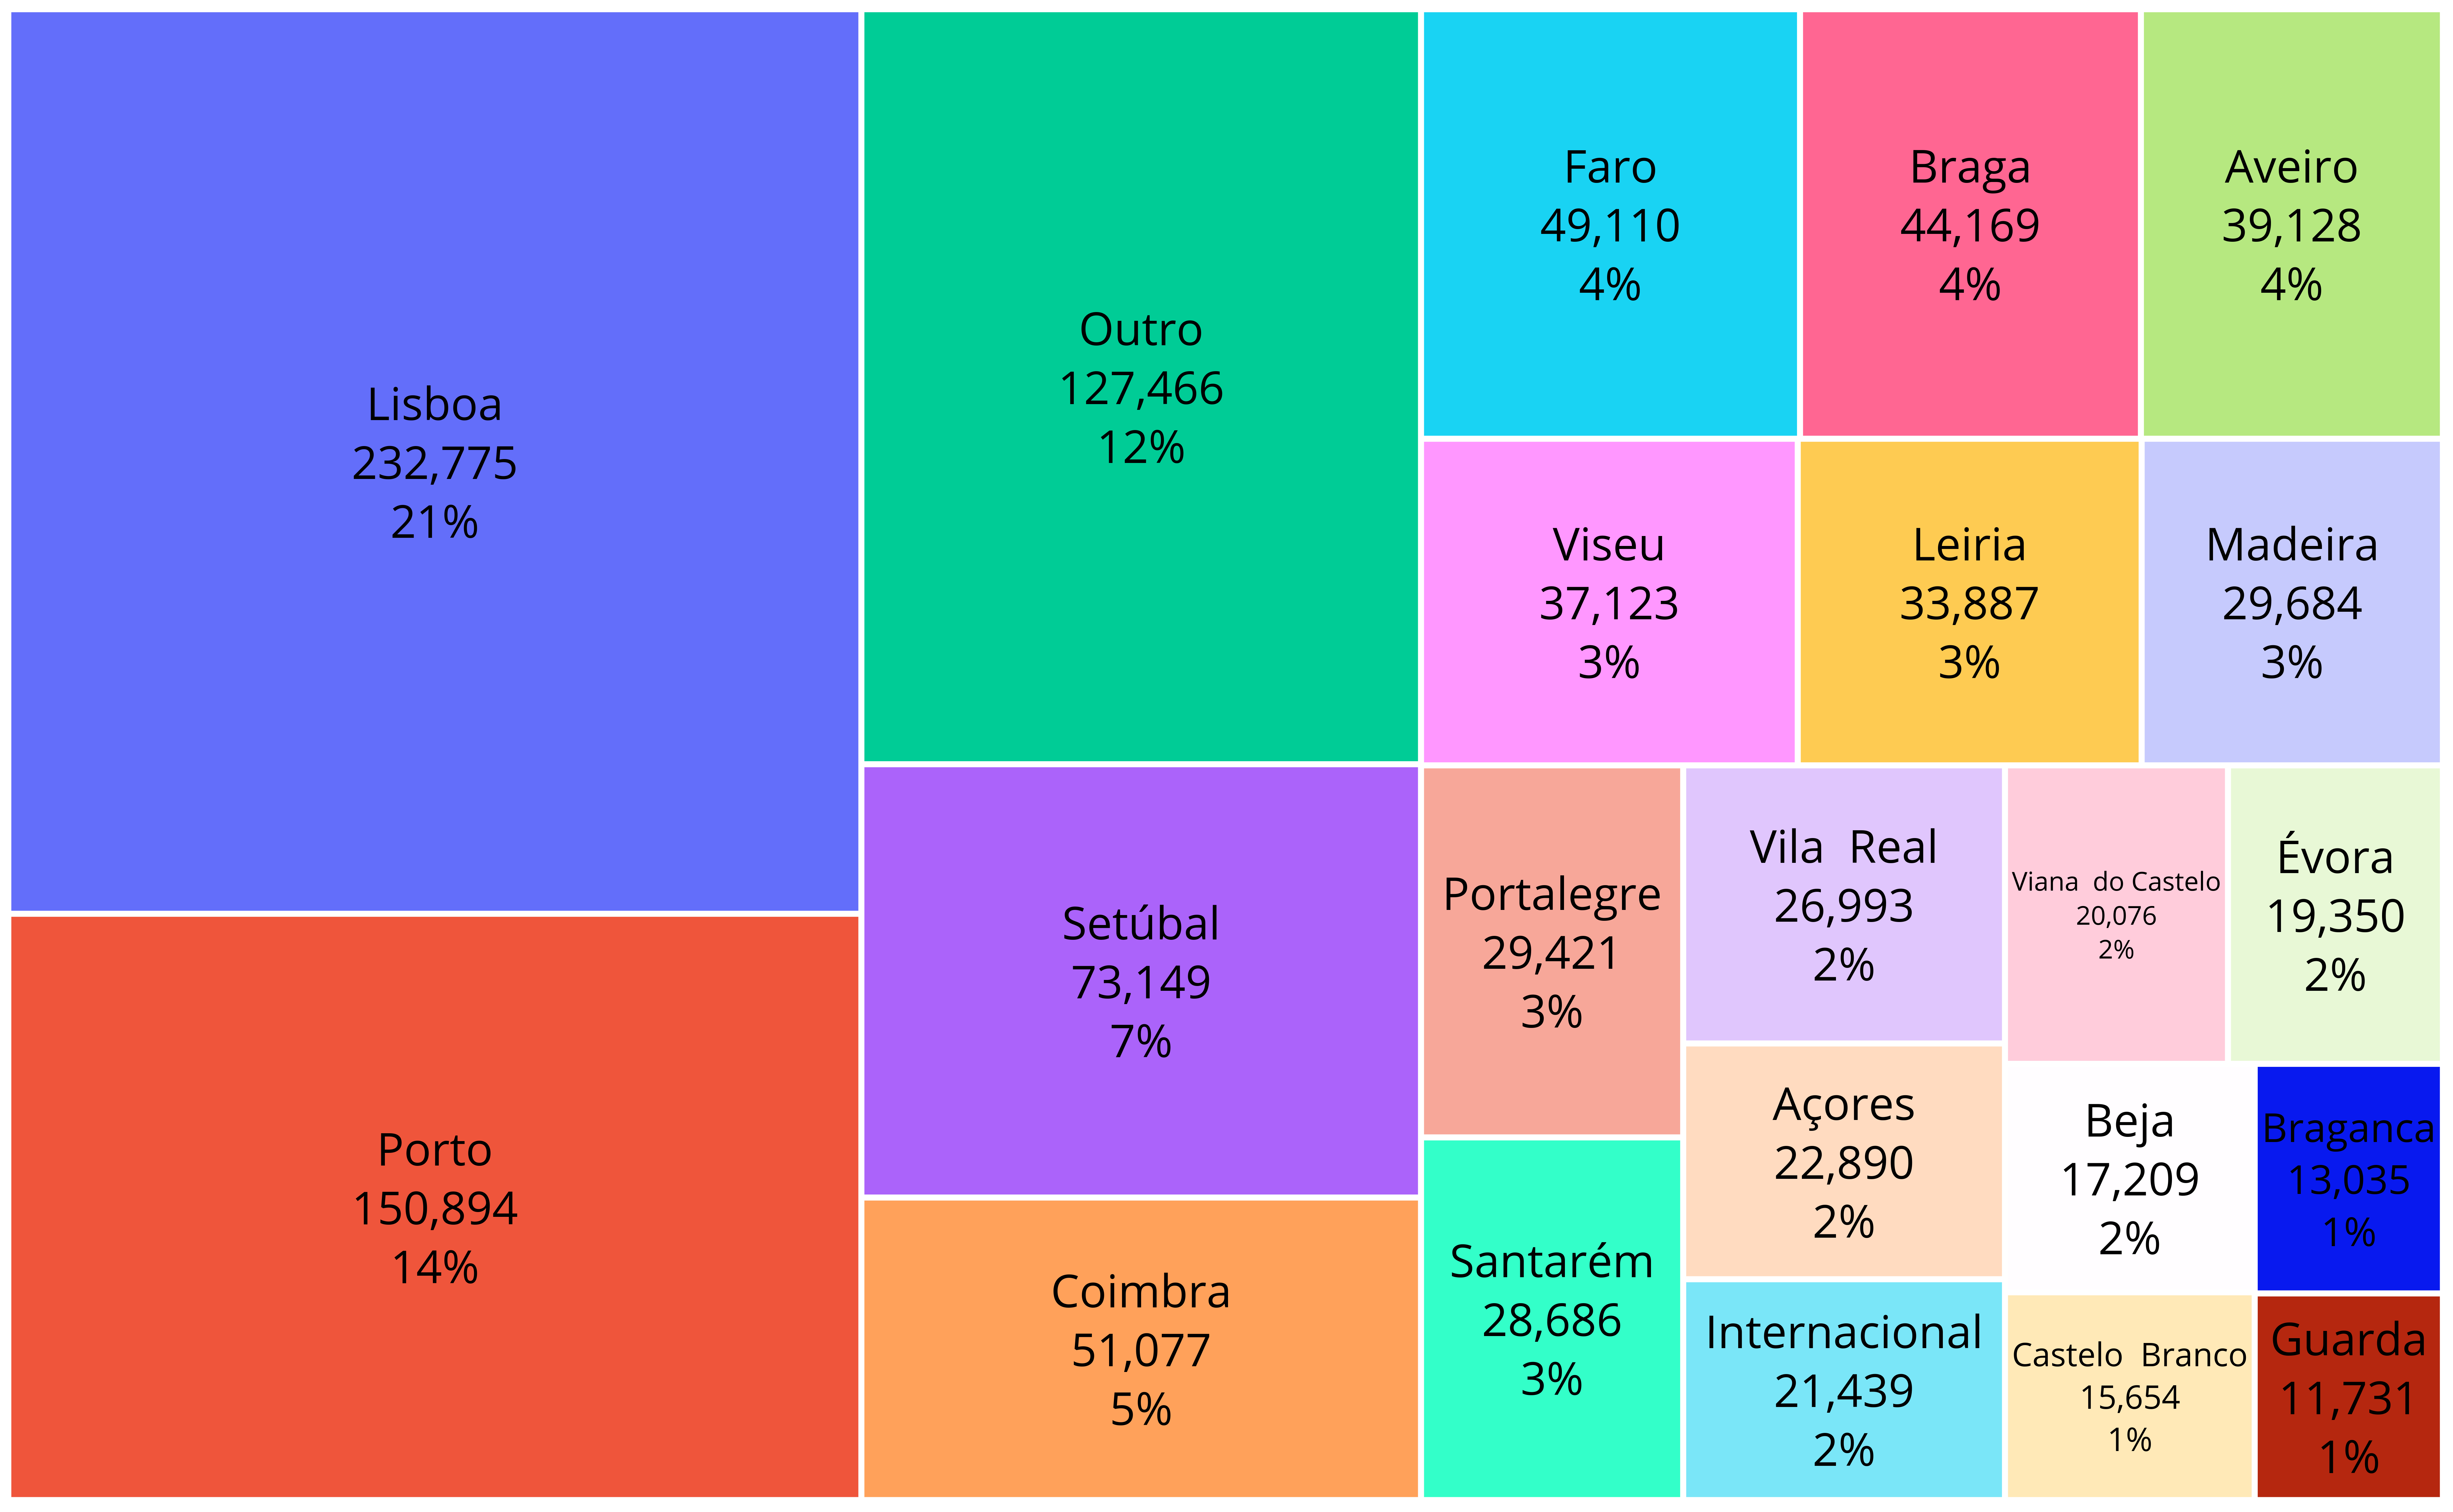
\includegraphics[width=\textwidth]{imagens/treemap_distritos.png}
	\caption{Distribuição do número de contratos públicos por distrito}
	\label{fig:distritos}
\end{figure}
\vfill 
\begin{figure}[H]
	\centering
	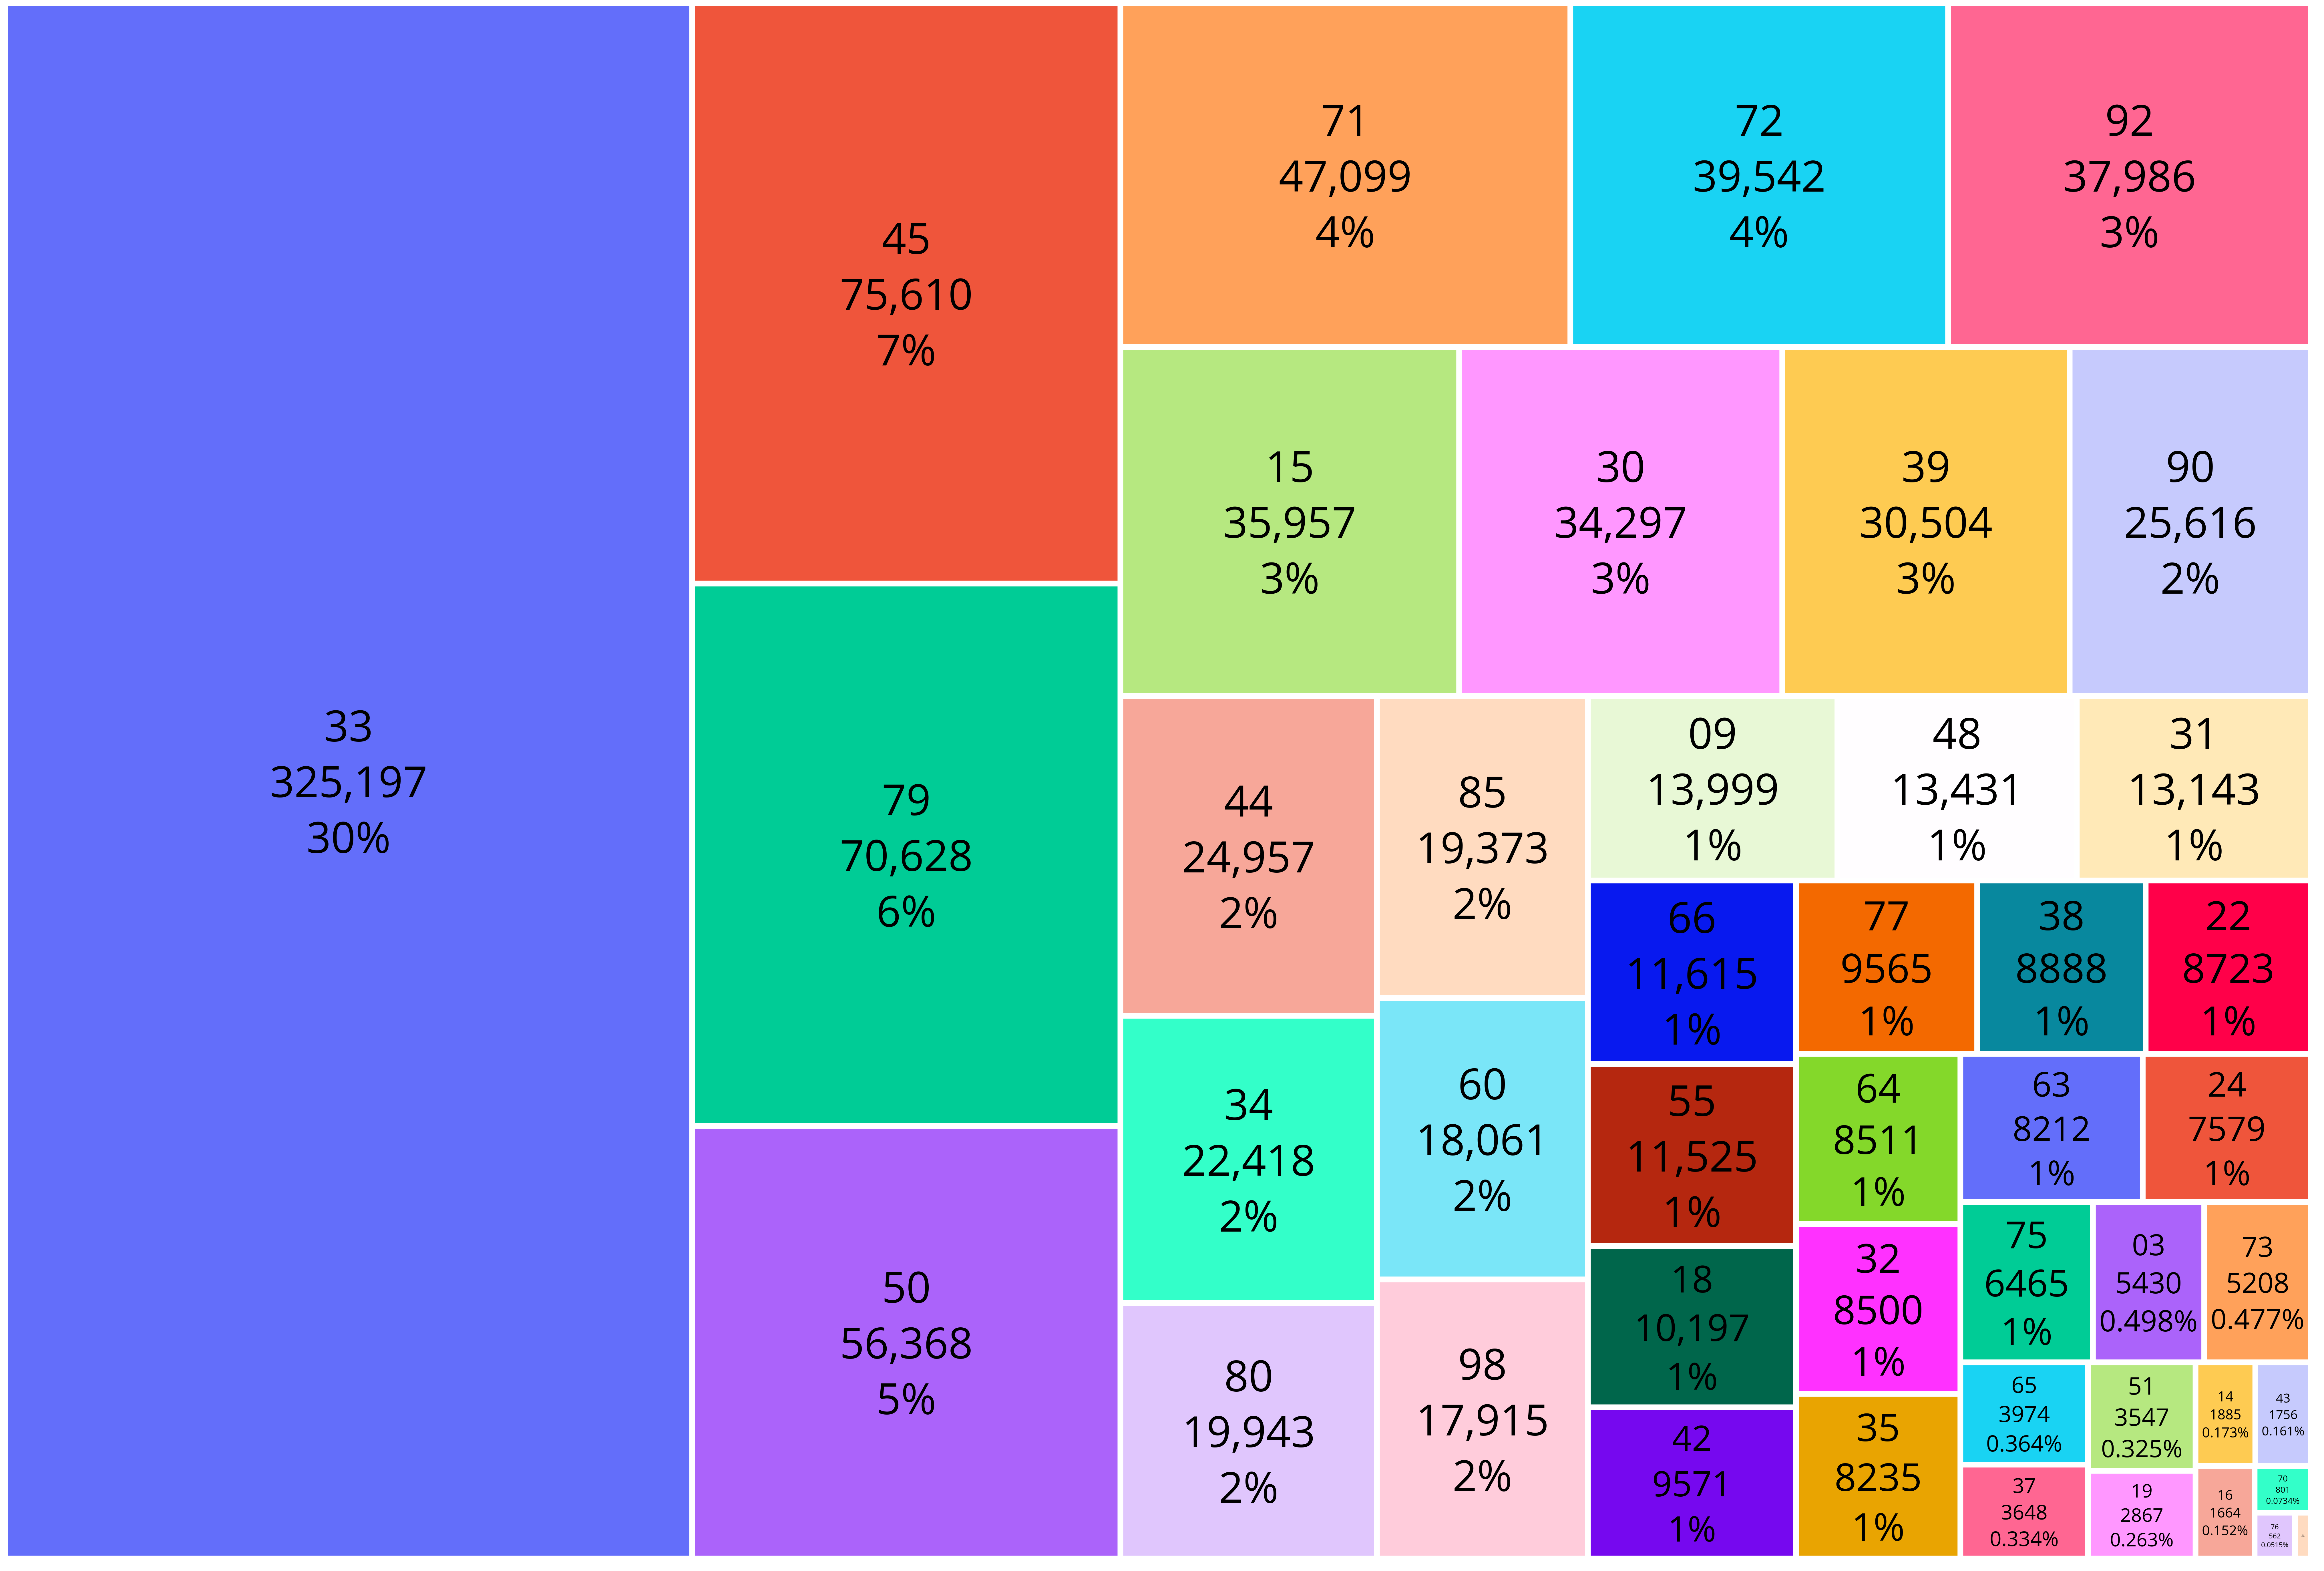
\includegraphics[width=\textwidth]{imagens/treemap_contratos.png}
	\caption{Distribuição do número de contratos públicos por divisão de CPV}
	\label{fig:cpvs}
\end{figure}
\vfill
\clearpage


\begin{wrapfigure}{R}{0.49\textwidth}
	\centering
	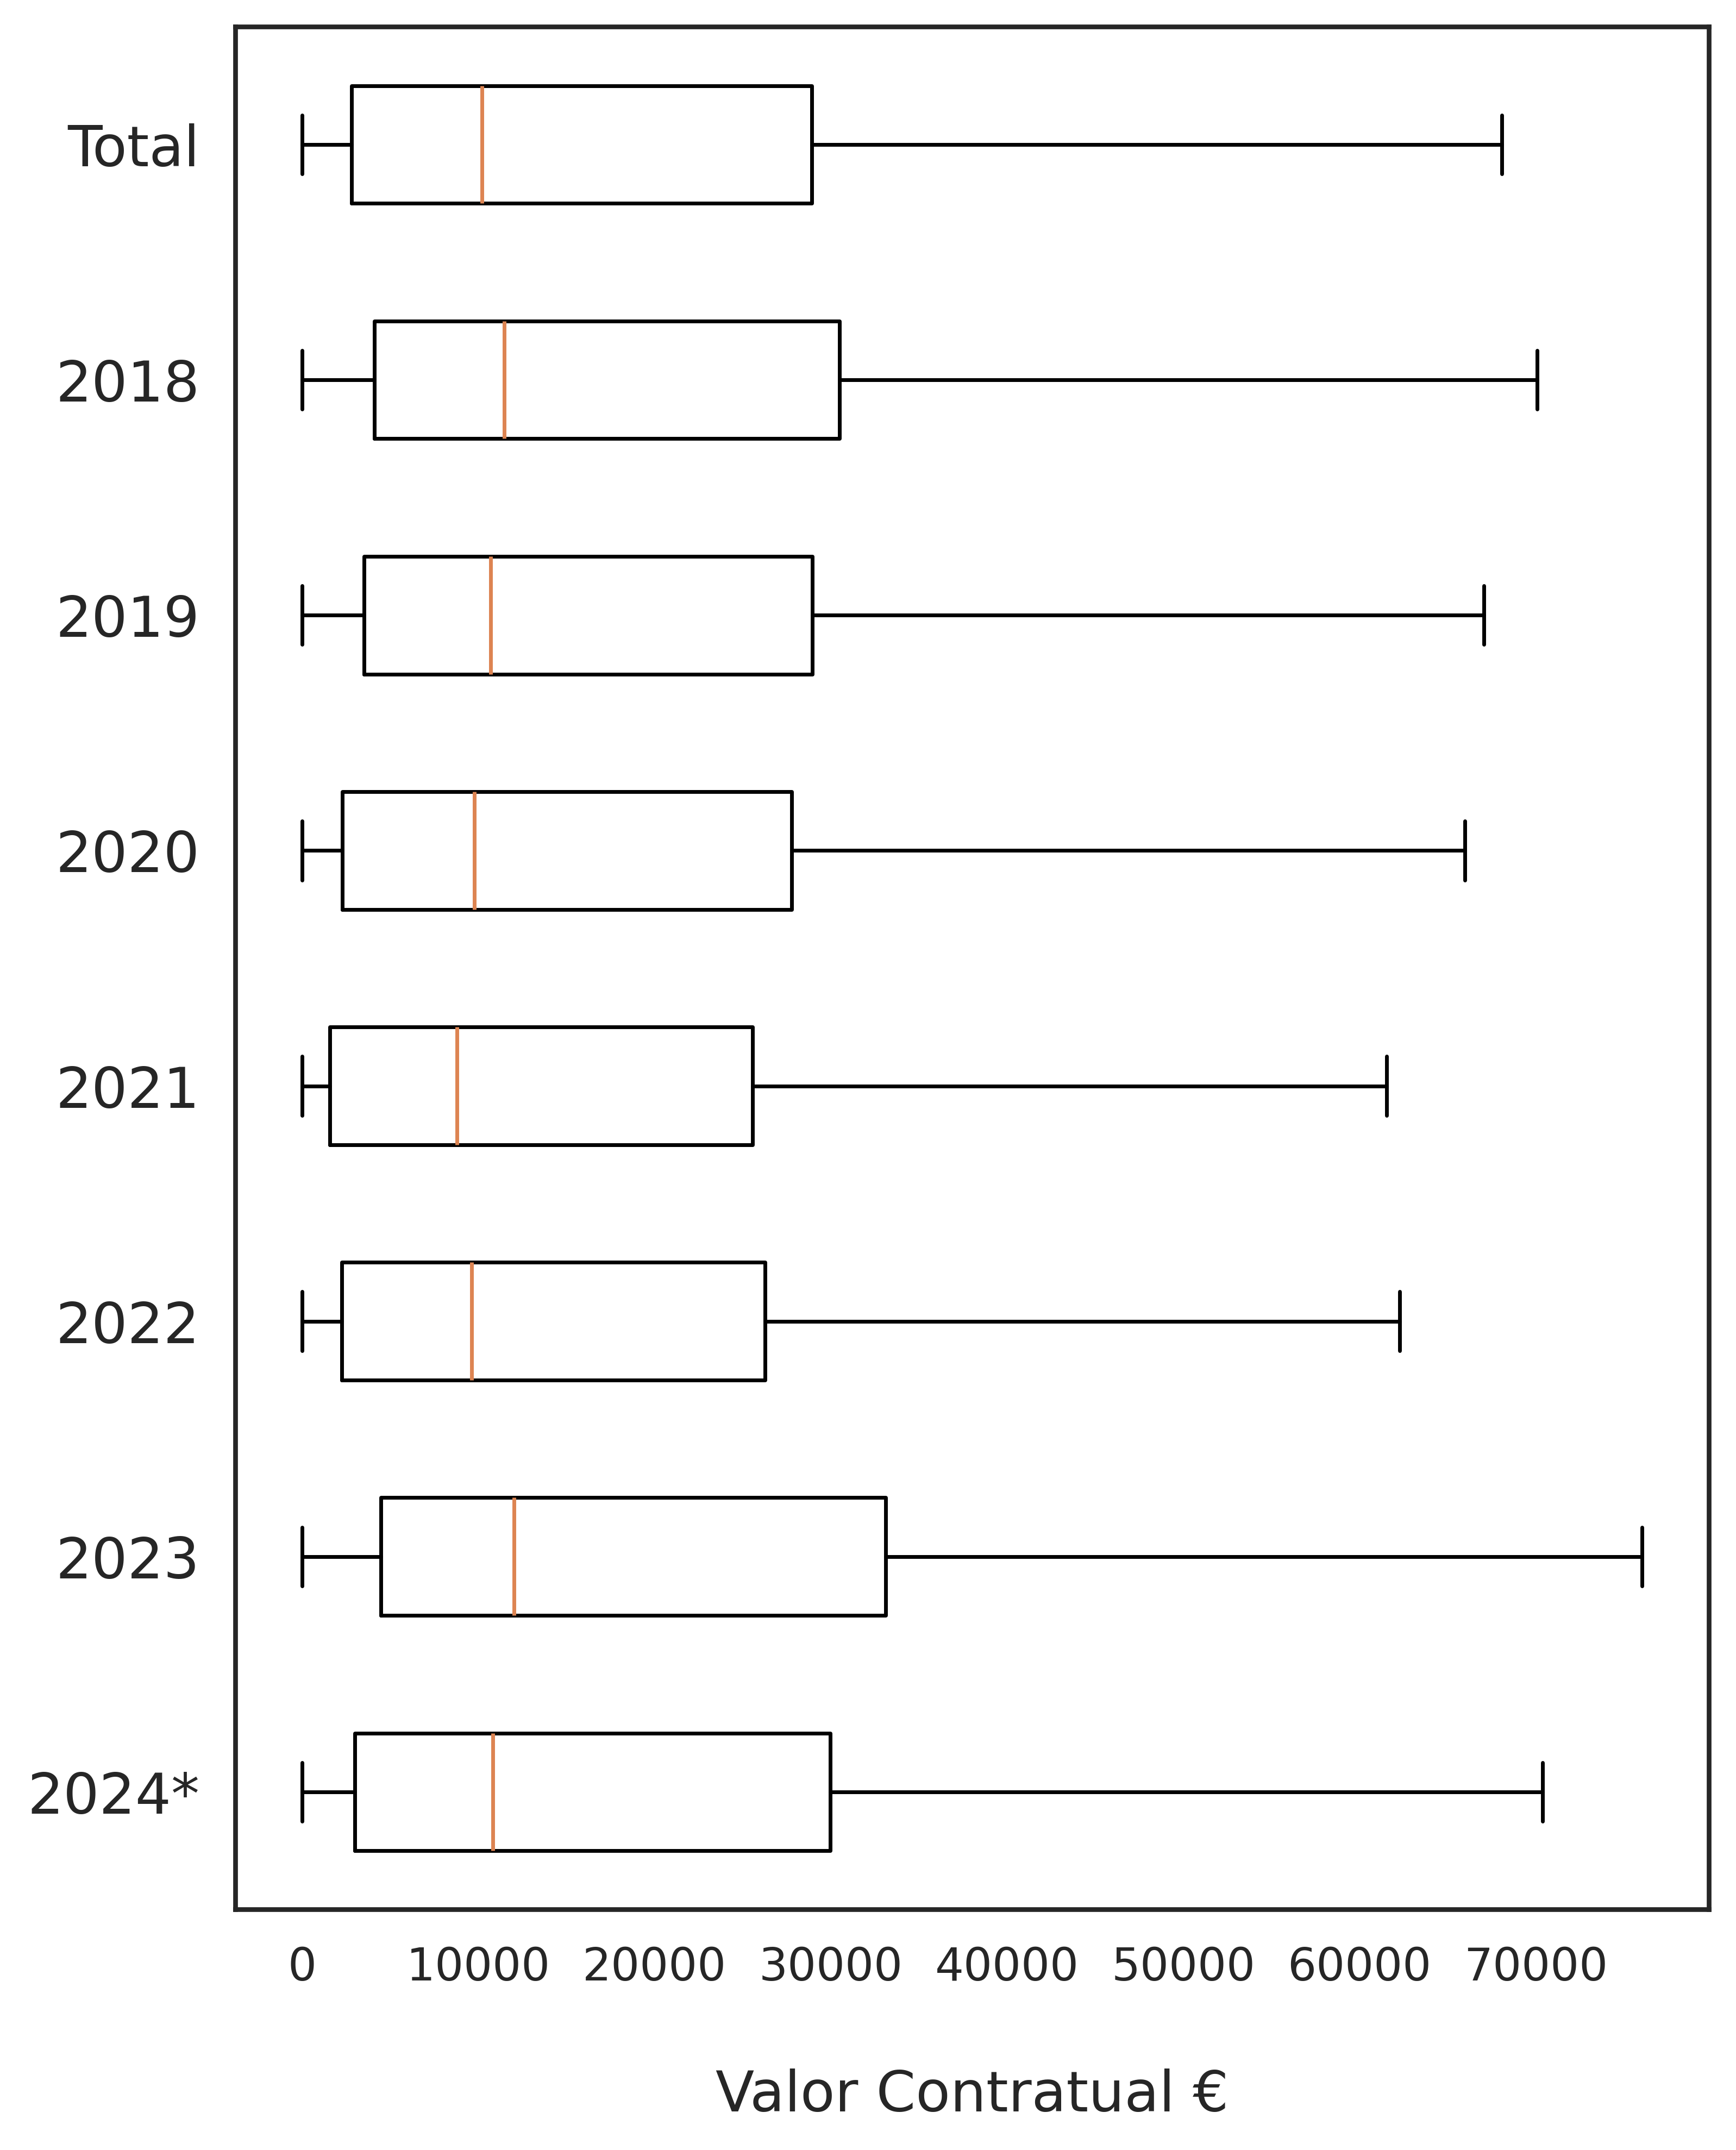
\includegraphics[width=0.49\textwidth]{imagens/precoscontr_stat.png}
	\caption{Boxplot dos preços contratuais para toda a tipologia de contratos desde 2018 até 2024}
	\label{fig:precotodos}
\end{wrapfigure}


Outra das variáveis com especial importância ao longo do projeto é o preço contratual. A Figura \ref{fig:precotodos} representa os boxplots referentes aos preços contratuais para todos os contratos da base de dados, independentemente da tipologia de procedimento, entre os anos de 2018 e 2024 e durante o período de tempo total ( de 2018 a 2024 ). É importante salientar que, tendo em conta que existem 2672 contratos cujo preço contratual é nulo, estes gráficos são meramente ilustrativos e existe um desfasamento entre a informação aqui apresentada e os valores reais. Pode-se observar que os valores dos 1º, 2º e 3º quartis tomam, sensivelmente, valores próximos. A distância interquantil permite-nos também constatar que, por ano, 50\% dos contratos têm um preço contratual compreendido no mesmo intervalo. Porém, tendo em conta que estamos a ter em conta em todas as tipologias de contratos e todas as divisões de CPV, esta informação é pouco informativa. Evidentemente, contratos referentes à construção civil (45) são celebrados com valores bastante diferentes de contratos referentes a serviços recreativos, culturais e despotivos (92). Por sua vez, tal como foi visto no capítulo anterior, existem valores contratuais máximos permitidos mediante a tipologia de contrato. Desta forma, é natural que exista um elevado número de \textit{outliers}, não representados, nesta Figura. \\
Ao longo deste estágio foram apenas analisadas e estudadas duas tipologias de contratos: Ajustes Diretos em Regime Geral e Concursos Públicos. Dessa forma, é oportuno incluir alguma descrição estatística destes dois casos. Além dos boxplots, à semelhança dos representados na Figura \ref{fig:precotodos}, encontram-se representações gráficas relativas aos número de contratos e o respetivo preço contratual total, de cada uma das duas categorias e por ano. Os resultados encontram-se nas Figuras \ref{fig:precocps}, \ref{fig:precocps1} e \ref{fig:precocps2} para concursos públicos e nas Figuras \ref{fig:precoad}, \ref{fig:precoad1} e \ref{fig:precoad2} para ajustes diretos em regime geral. É possível observar, de forma imediata, que os valores contratuais de concursos públicos são substancialmente superiores aos dos ajustes diretos. O número de contratos celebrados por ano é sempre inferior para concursos públicos mas o valor adjudicado foi sempre superior ao dos ajustes diretos. No caso dos concursos públicos, 40\% dos contratos celebrados dizem respeito a apenas duas divisões de CPV:  23\% dos contratos celebrados são para aquisição de equipamento médico e 17\% a obras de contrução civil, sendo cerca de 25\% deles celebrados no distrito de Lisboa, 10\% no Porto e 11\% em distrito indeterminado. Relativamente a ajustes diretos, existe, novamente, uma predominância de contratos referentes a aquisição de equipamento médico, totalizando 28\% de contratos celebrados, com maior destaque nos distritos de Lisboa, 23\%, e Porto, 17\%.


\begin{figure}[H]
	\centering
	\begin{minipage}{0.31\linewidth}
		%\centering  % redundant
		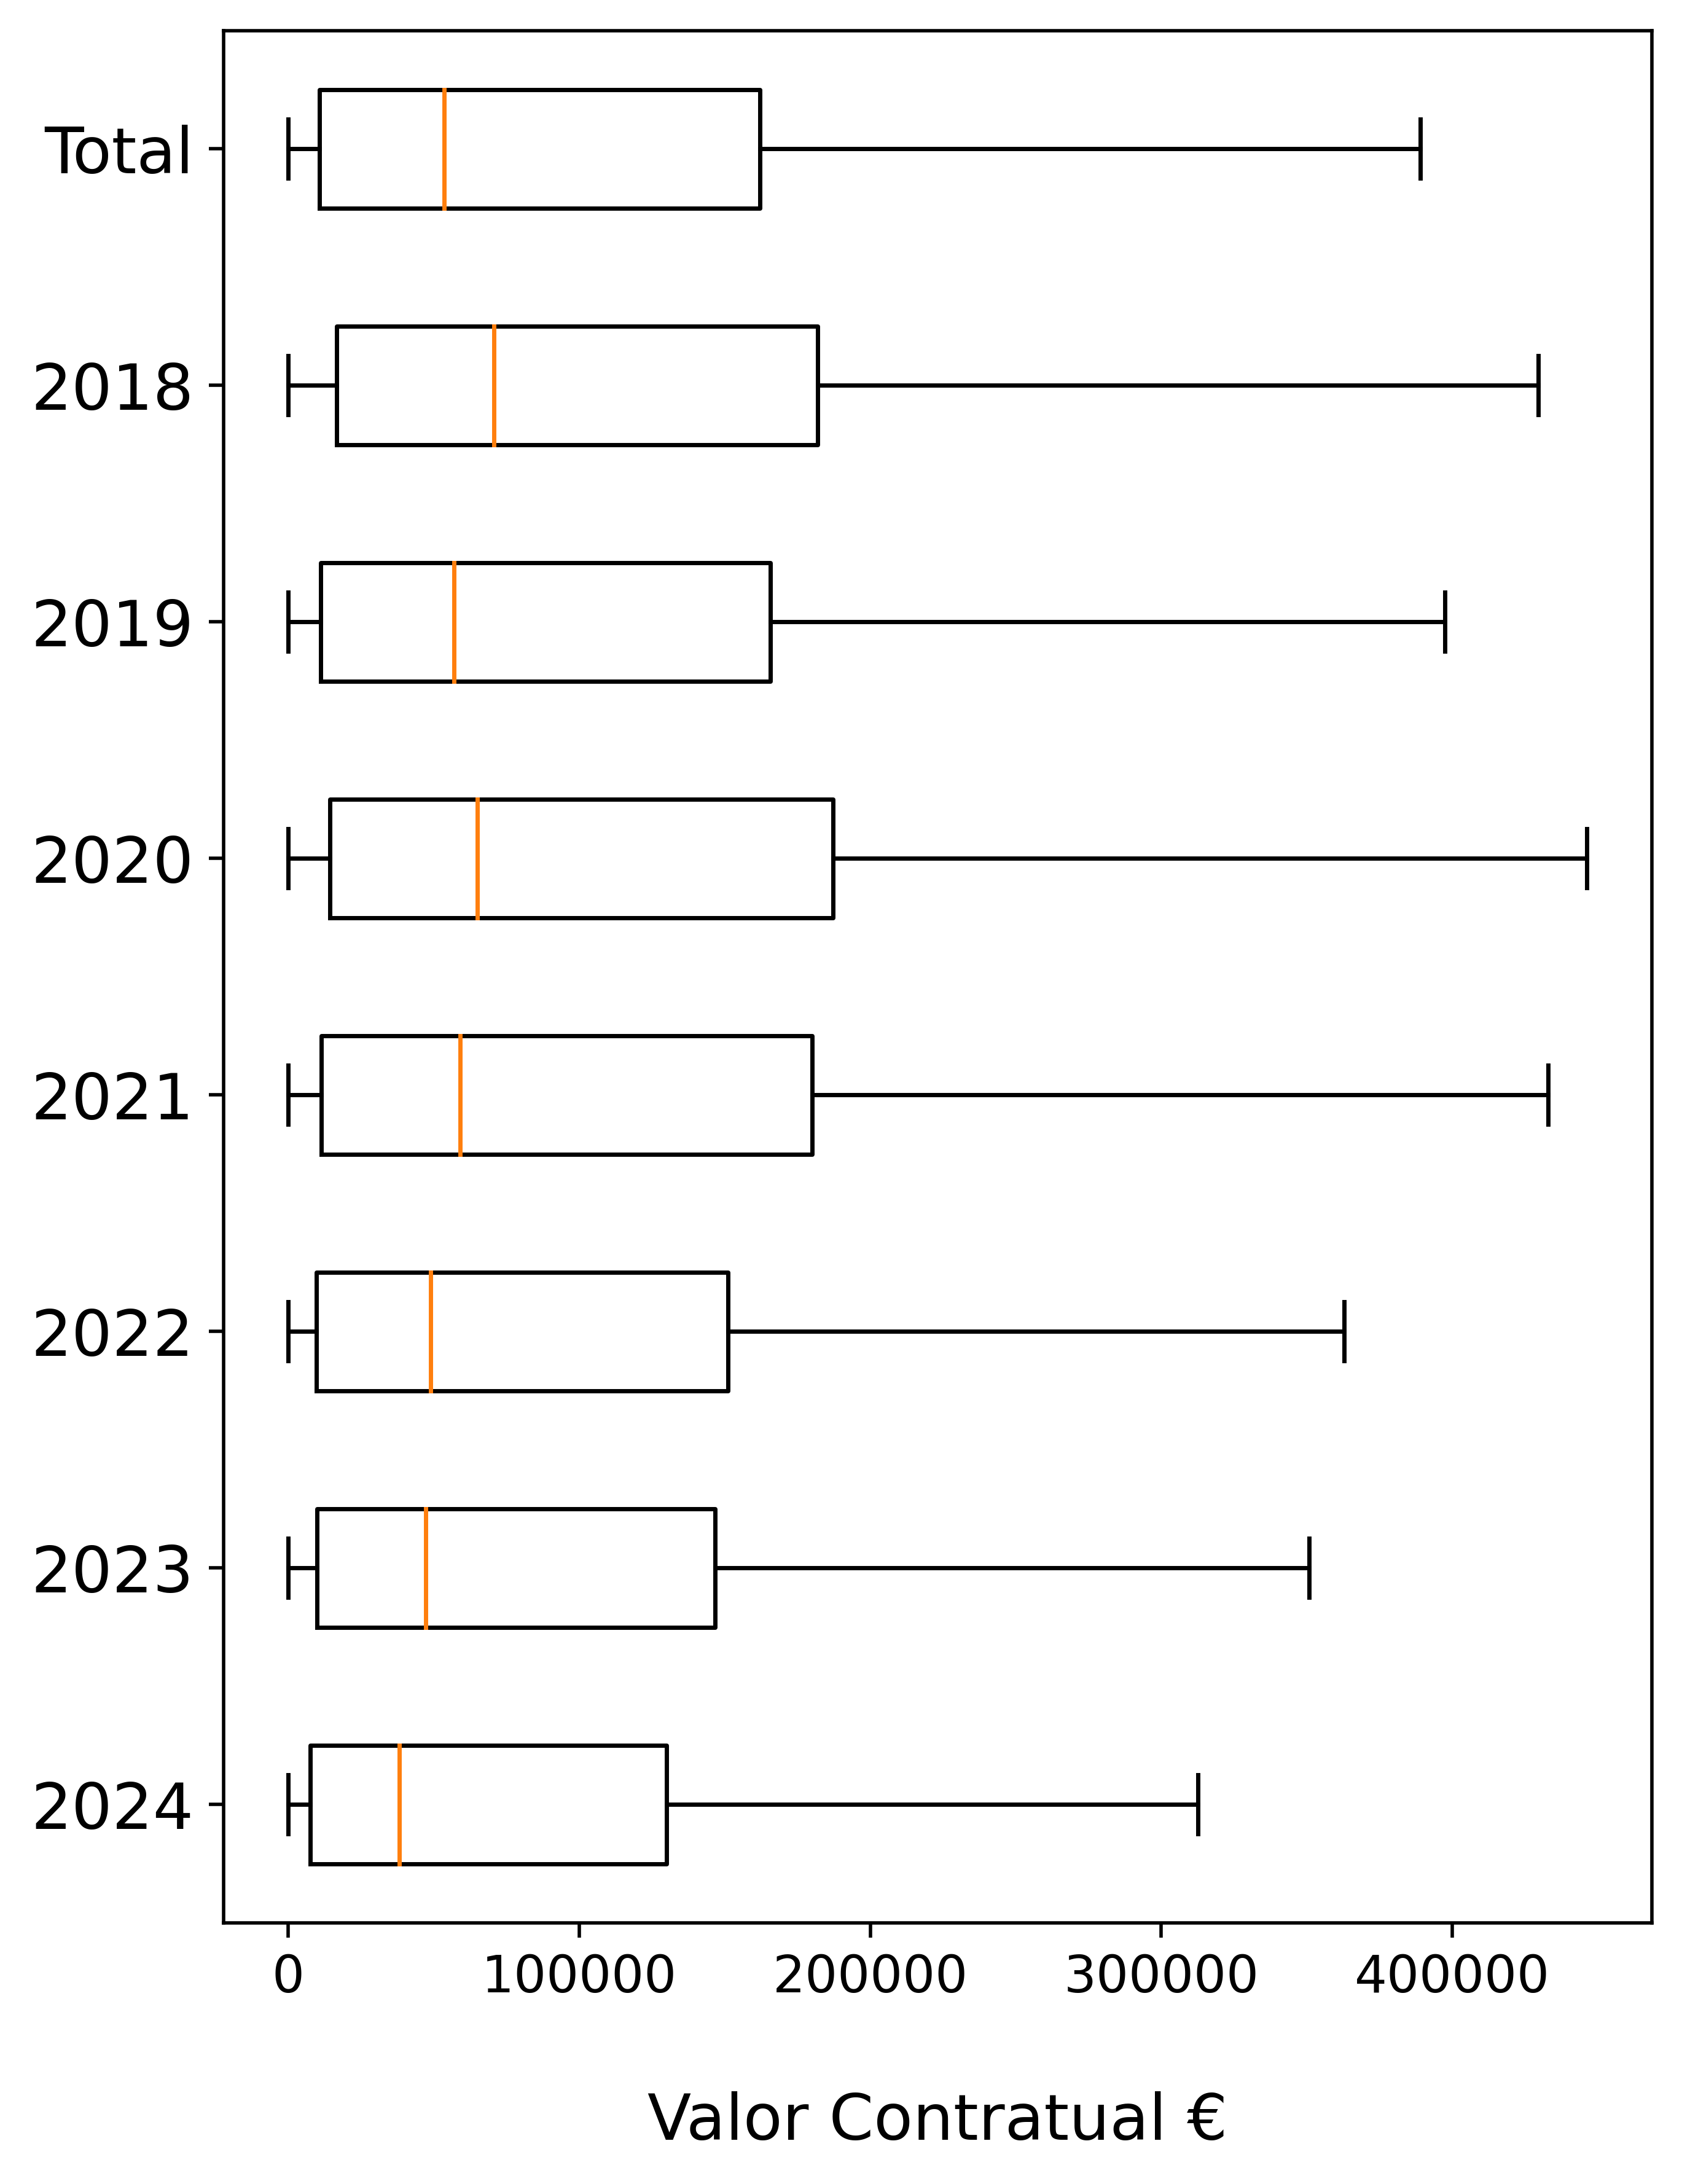
\includegraphics[width=\textwidth]{imagens/concpub_stat.png}
		\caption{Boxplot dos preços contratuais para concursos públicos desde 2018 até 2024}
		\label{fig:precocps}
	\end{minipage}
	\hfill
	\begin{minipage}{.31\linewidth}
		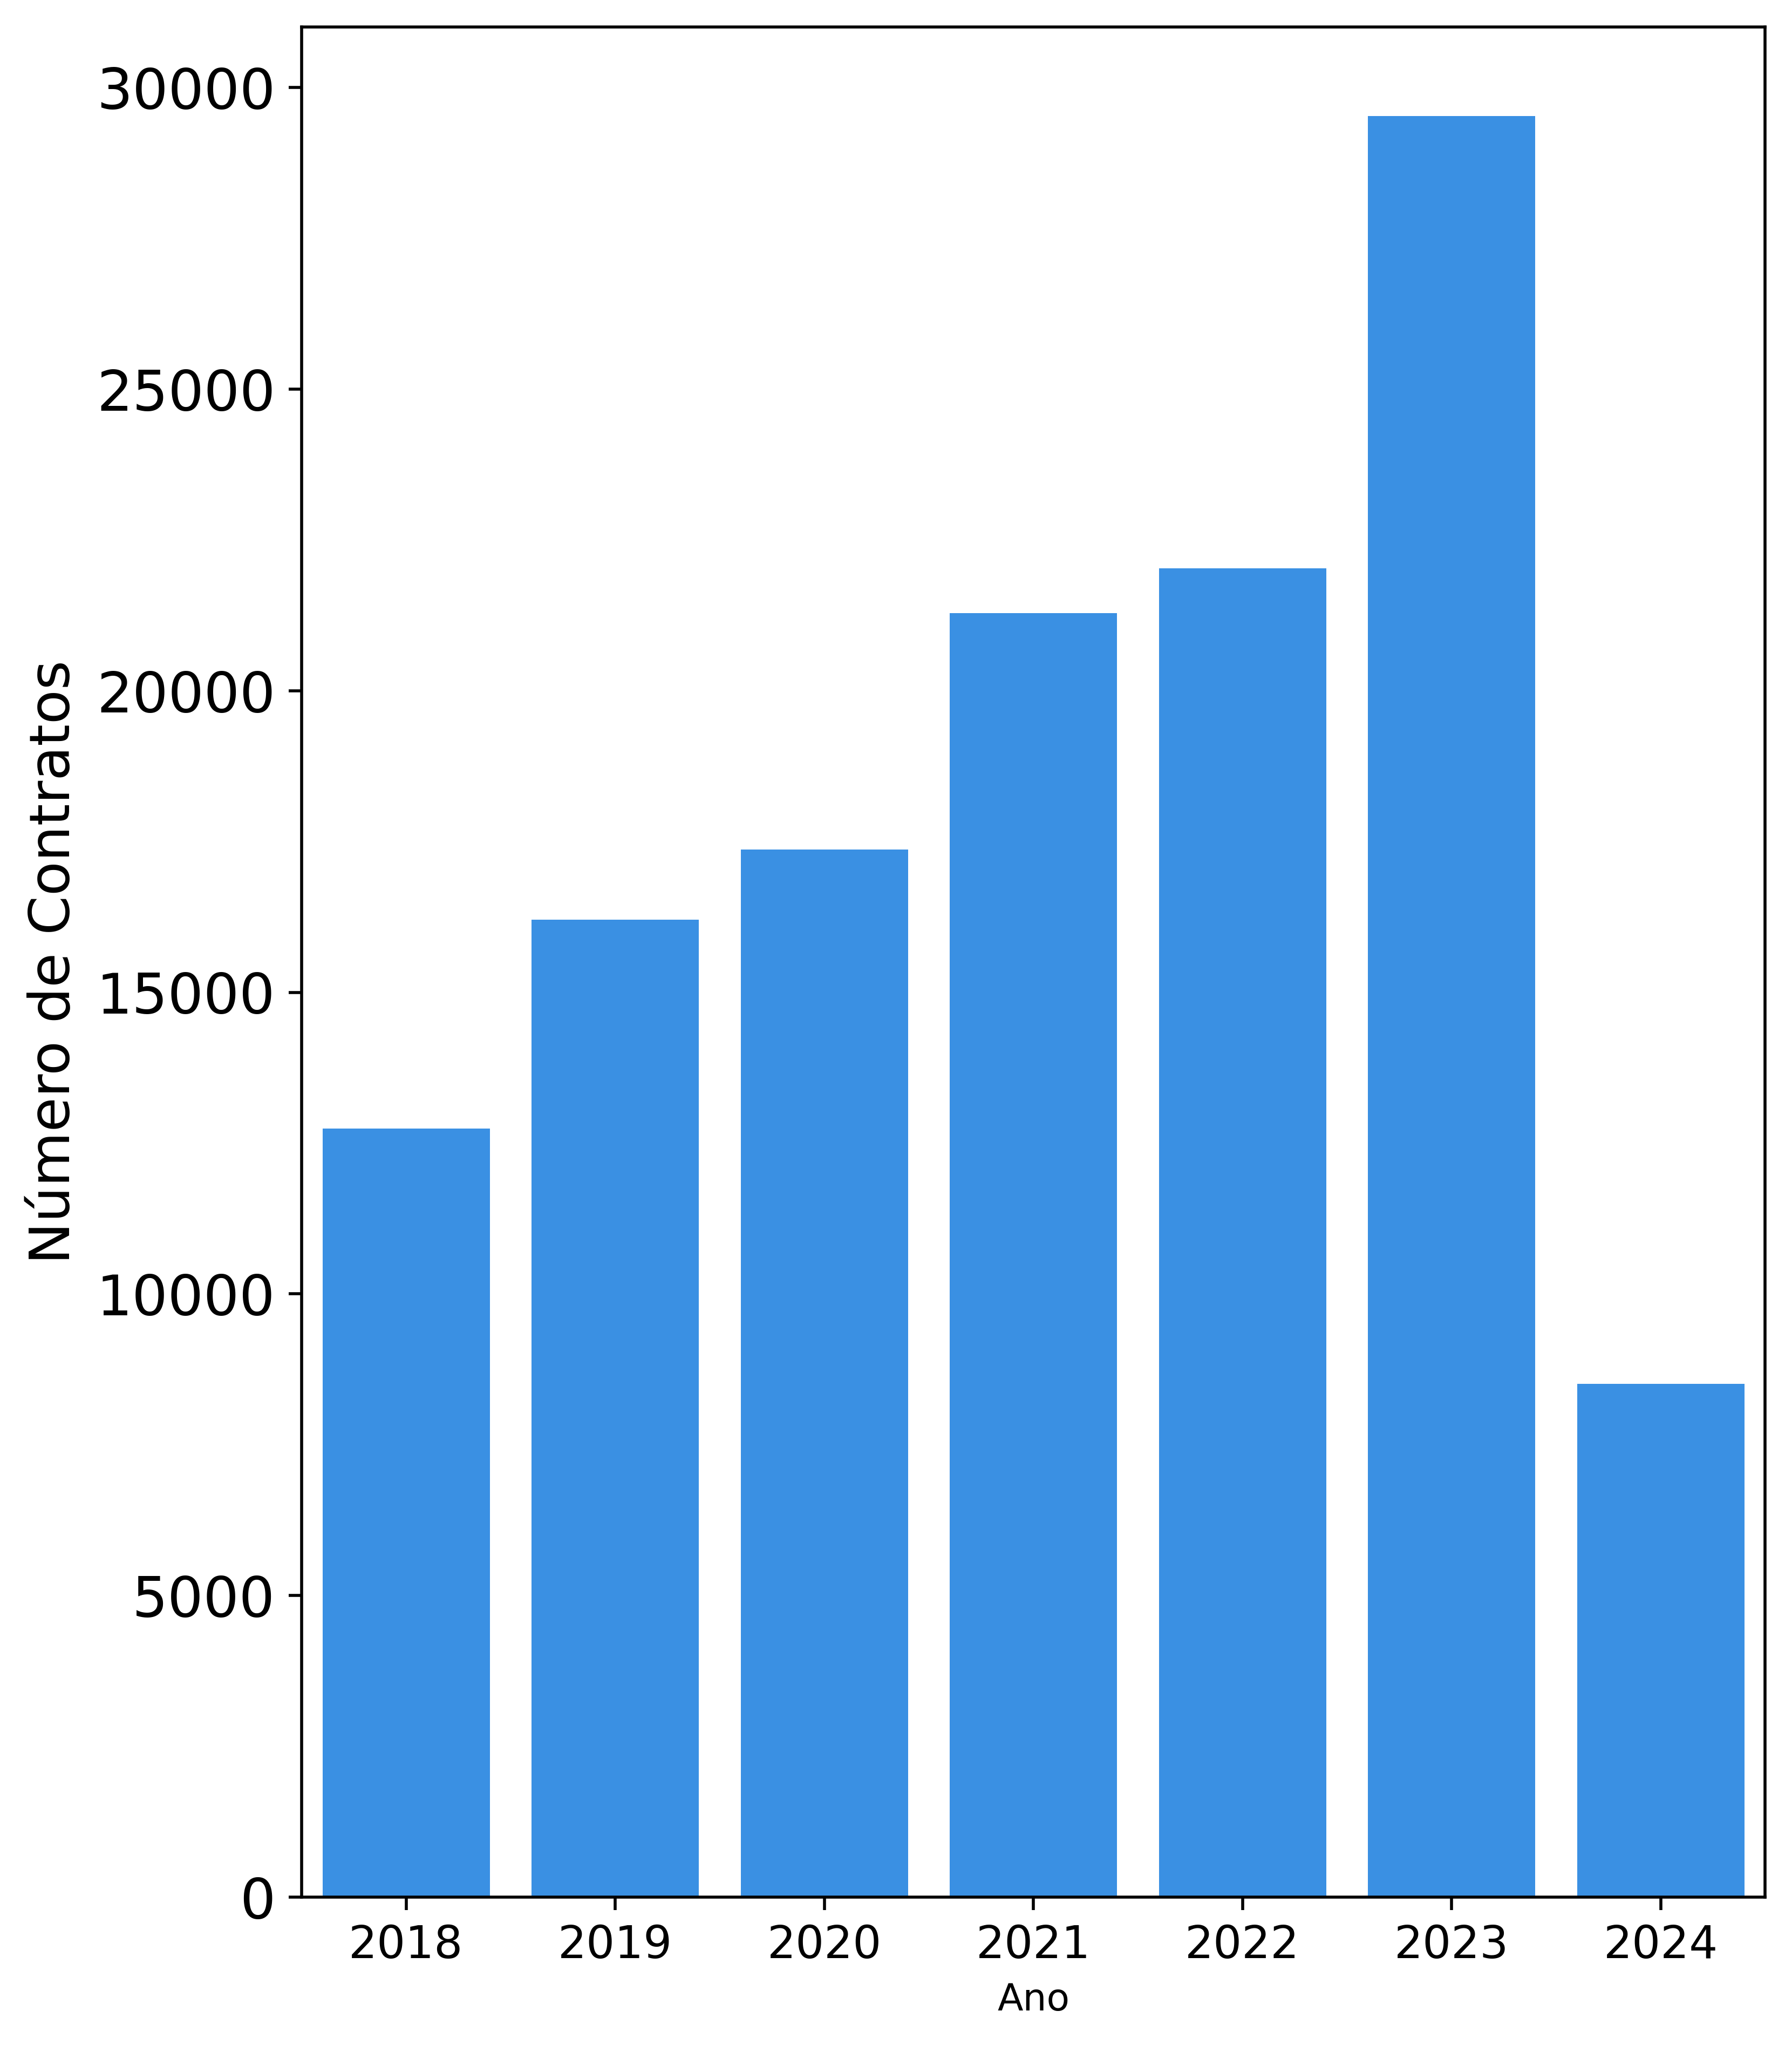
\includegraphics[width=\linewidth]{imagens/cpub_nrcontr.png}
		\caption{Número de concursos públicos celebradoss por ano, entre 2018 e 2024}
		\label{fig:precocps1}
	\end{minipage}
	\hfill
	\begin{minipage}{.31\linewidth}
		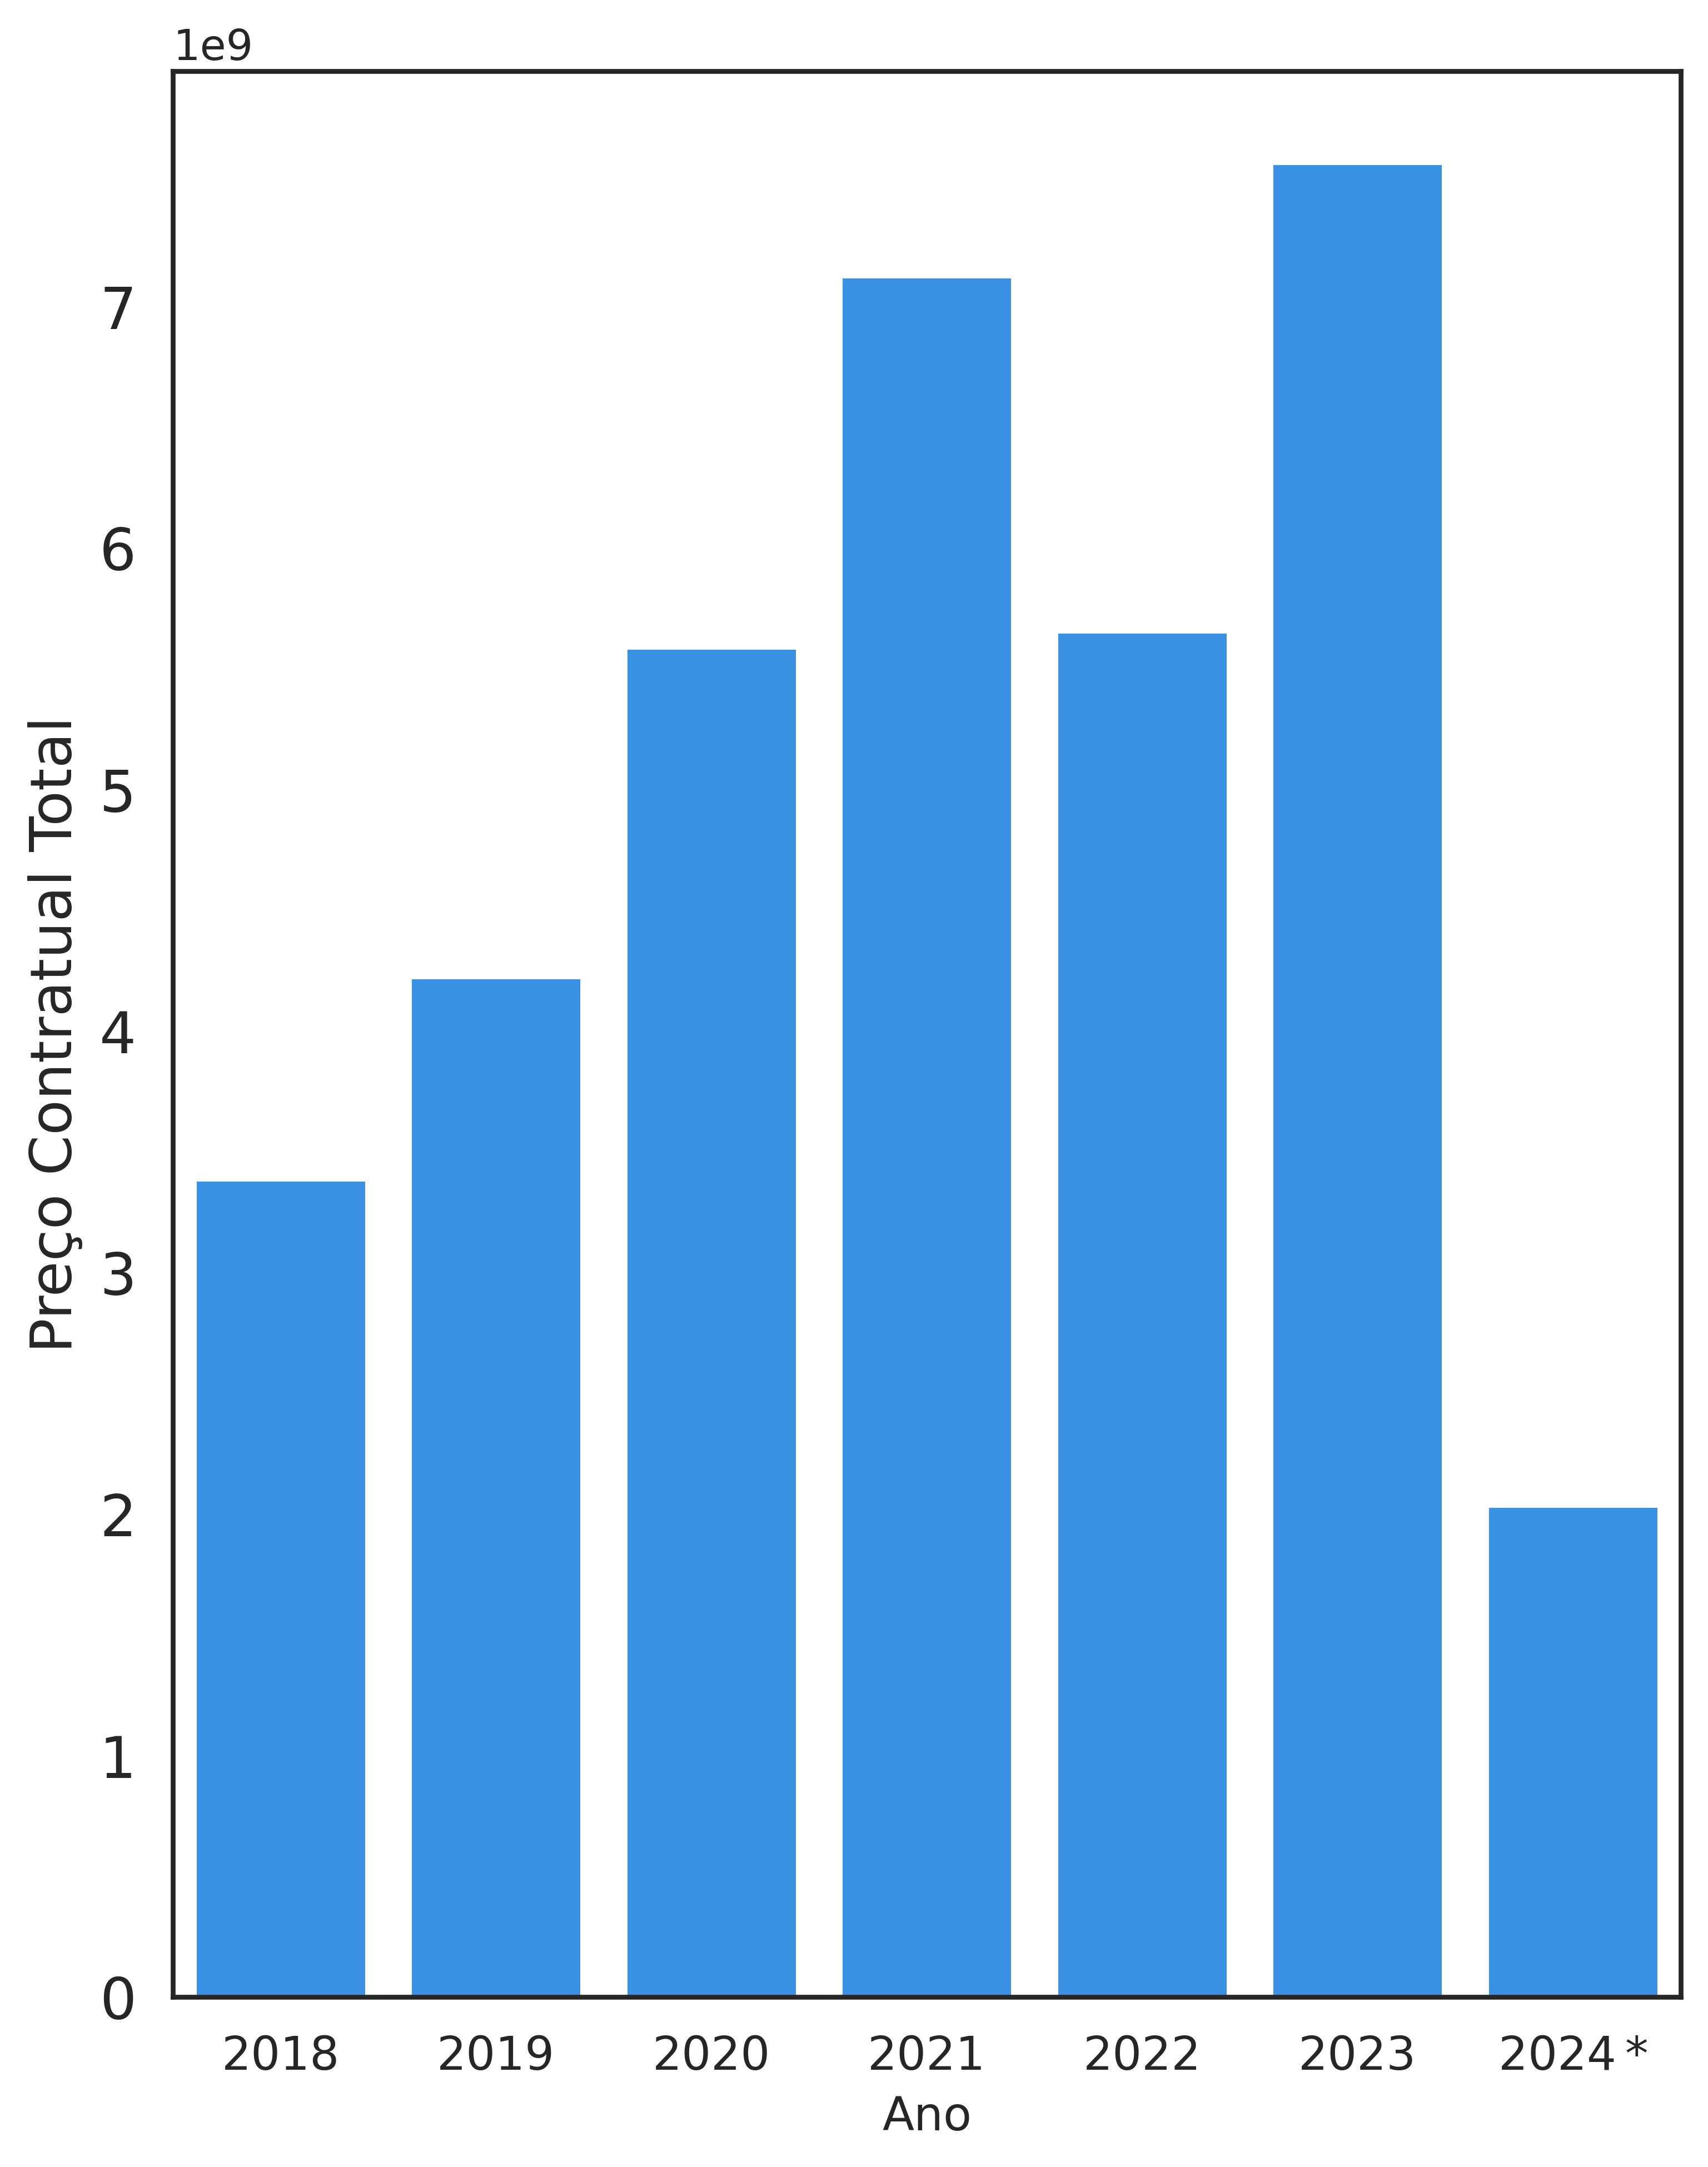
\includegraphics[width=\linewidth]{imagens/cpub_price.png}
		\caption{Preço contratual total por ano, entre 2018 e 2024, para concursos públicos}
		\label{fig:precocps2}
	\end{minipage}
\end{figure}


\begin{figure}[H]
	\centering
	\begin{minipage}{.31\linewidth}
		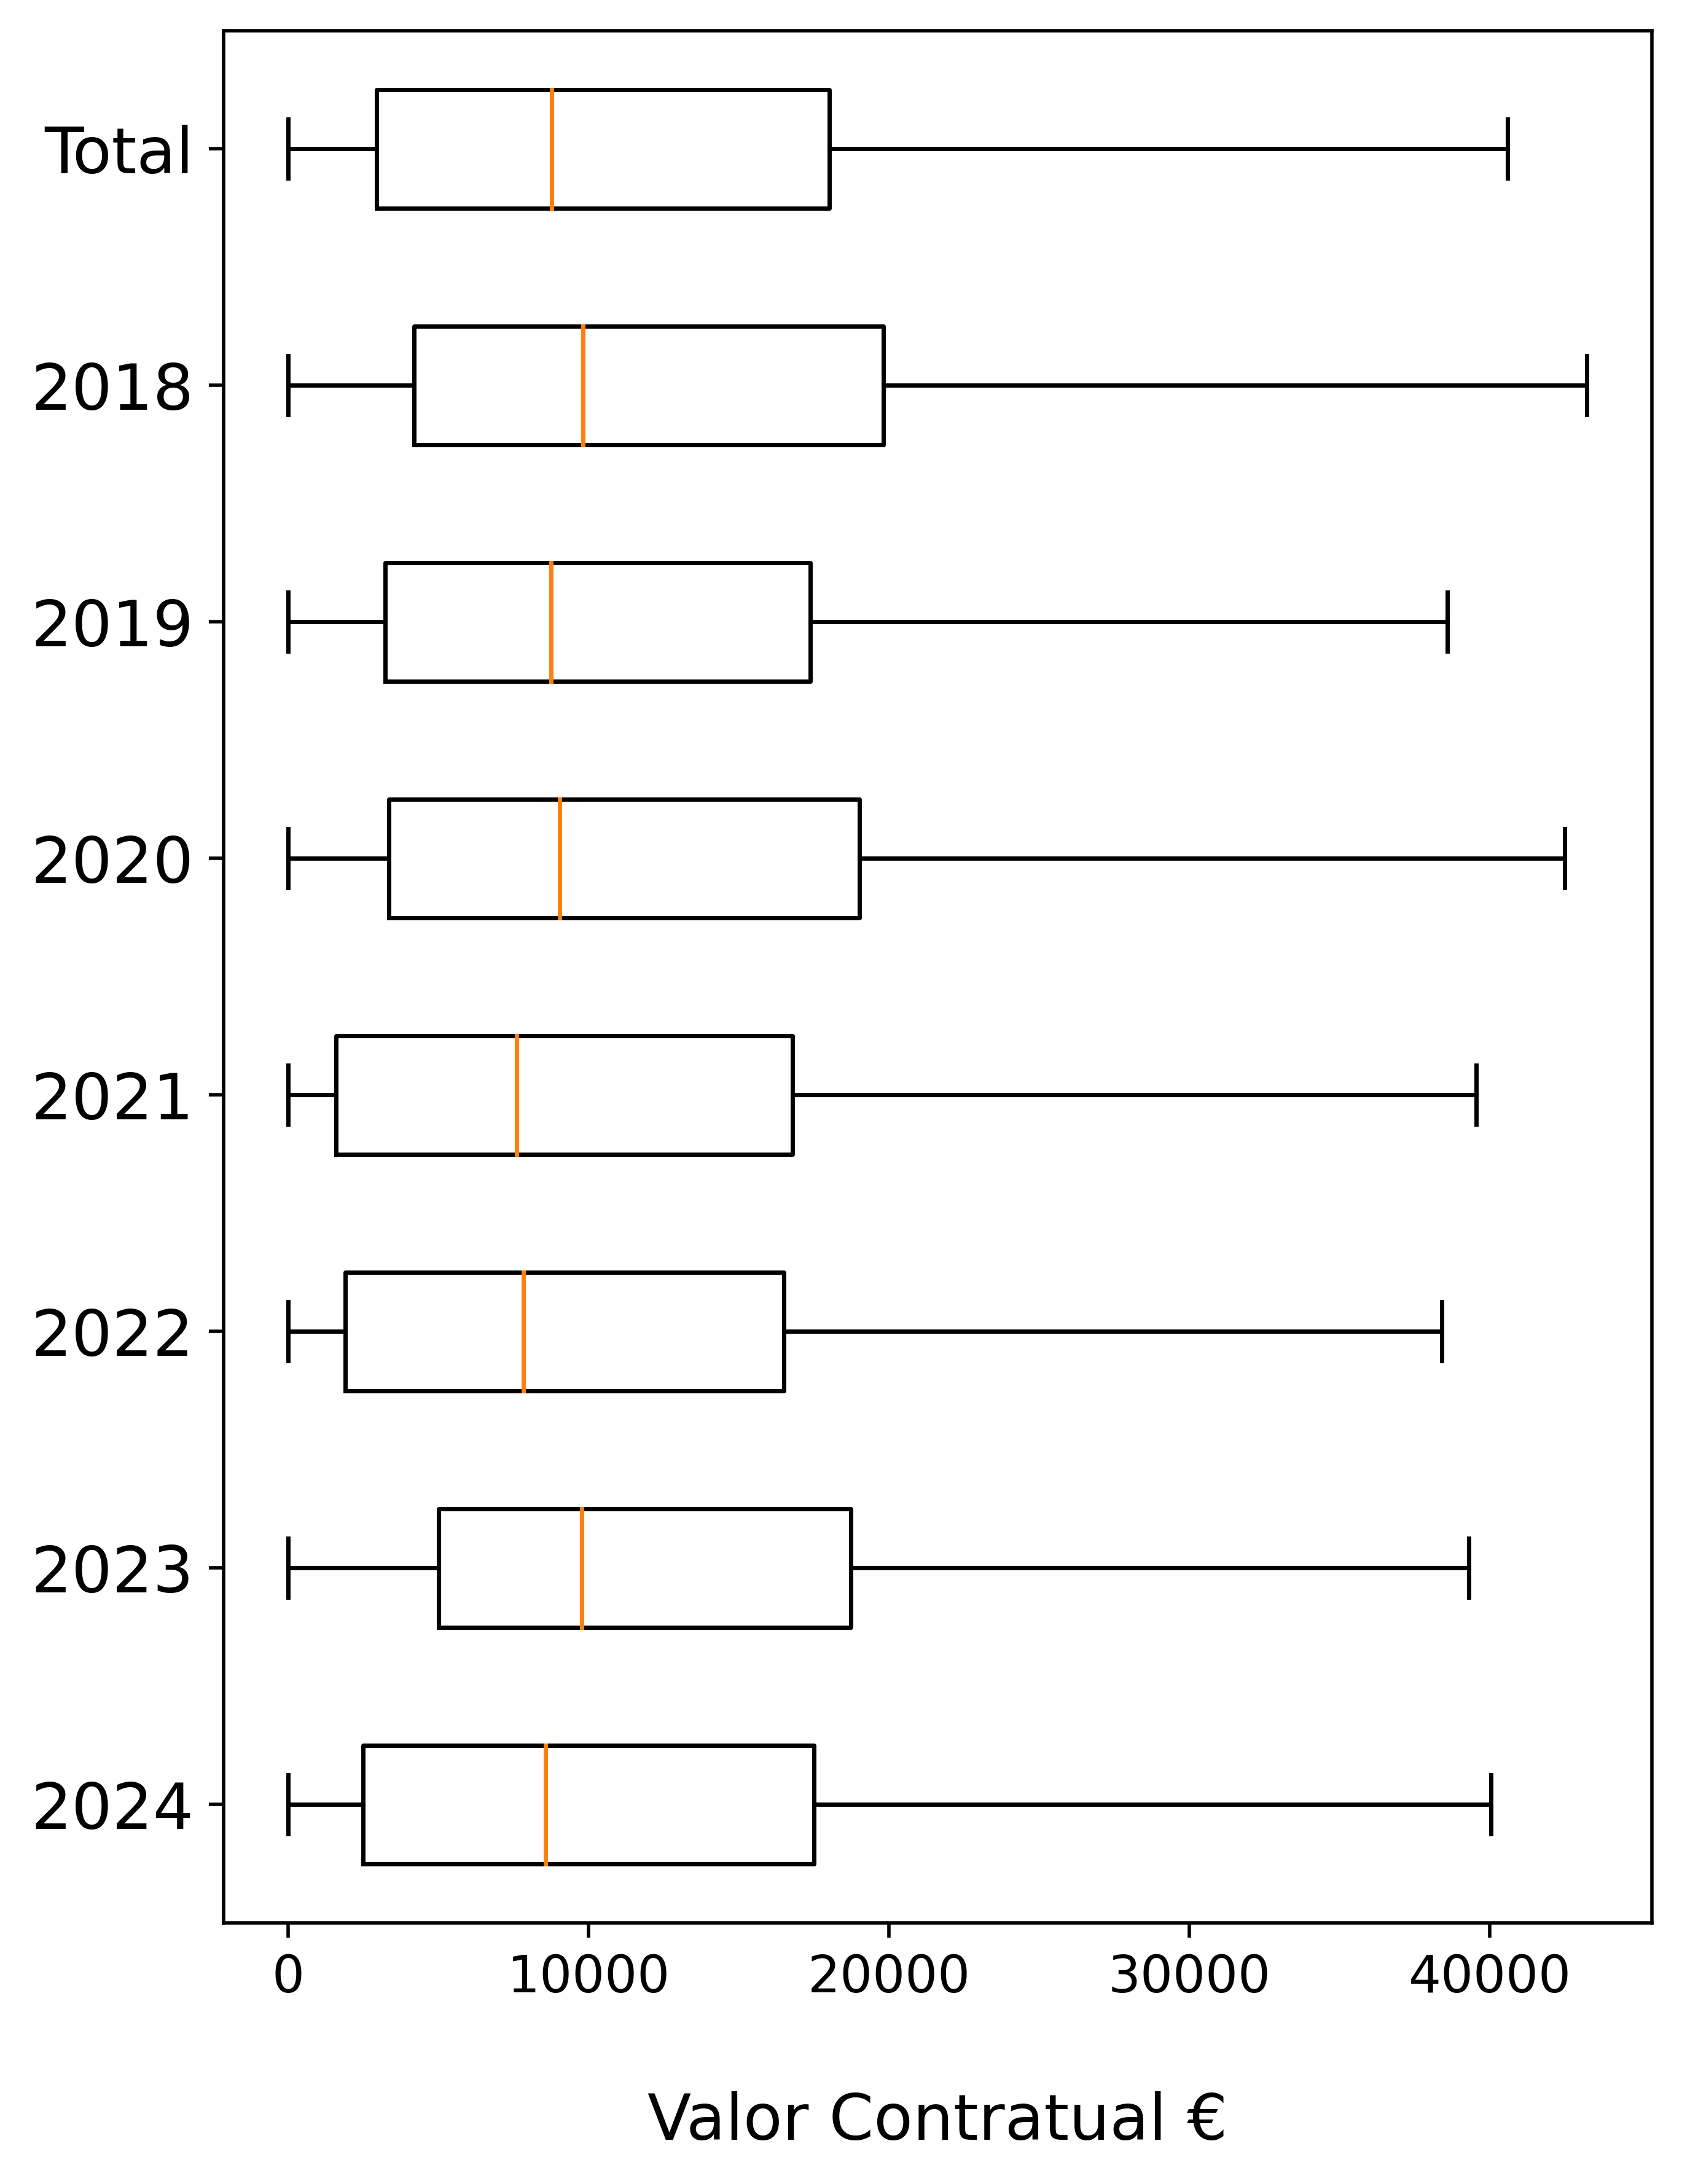
\includegraphics[width=\linewidth]{imagens/adir_stat.png}
		\caption{Número de concursos públicos celebradoss por ano, entre 2018 e 2024}
		\label{fig:precoad}
	\end{minipage}
	\hfill
	\begin{minipage}{0.31\linewidth}
		%\centering  % redundant
		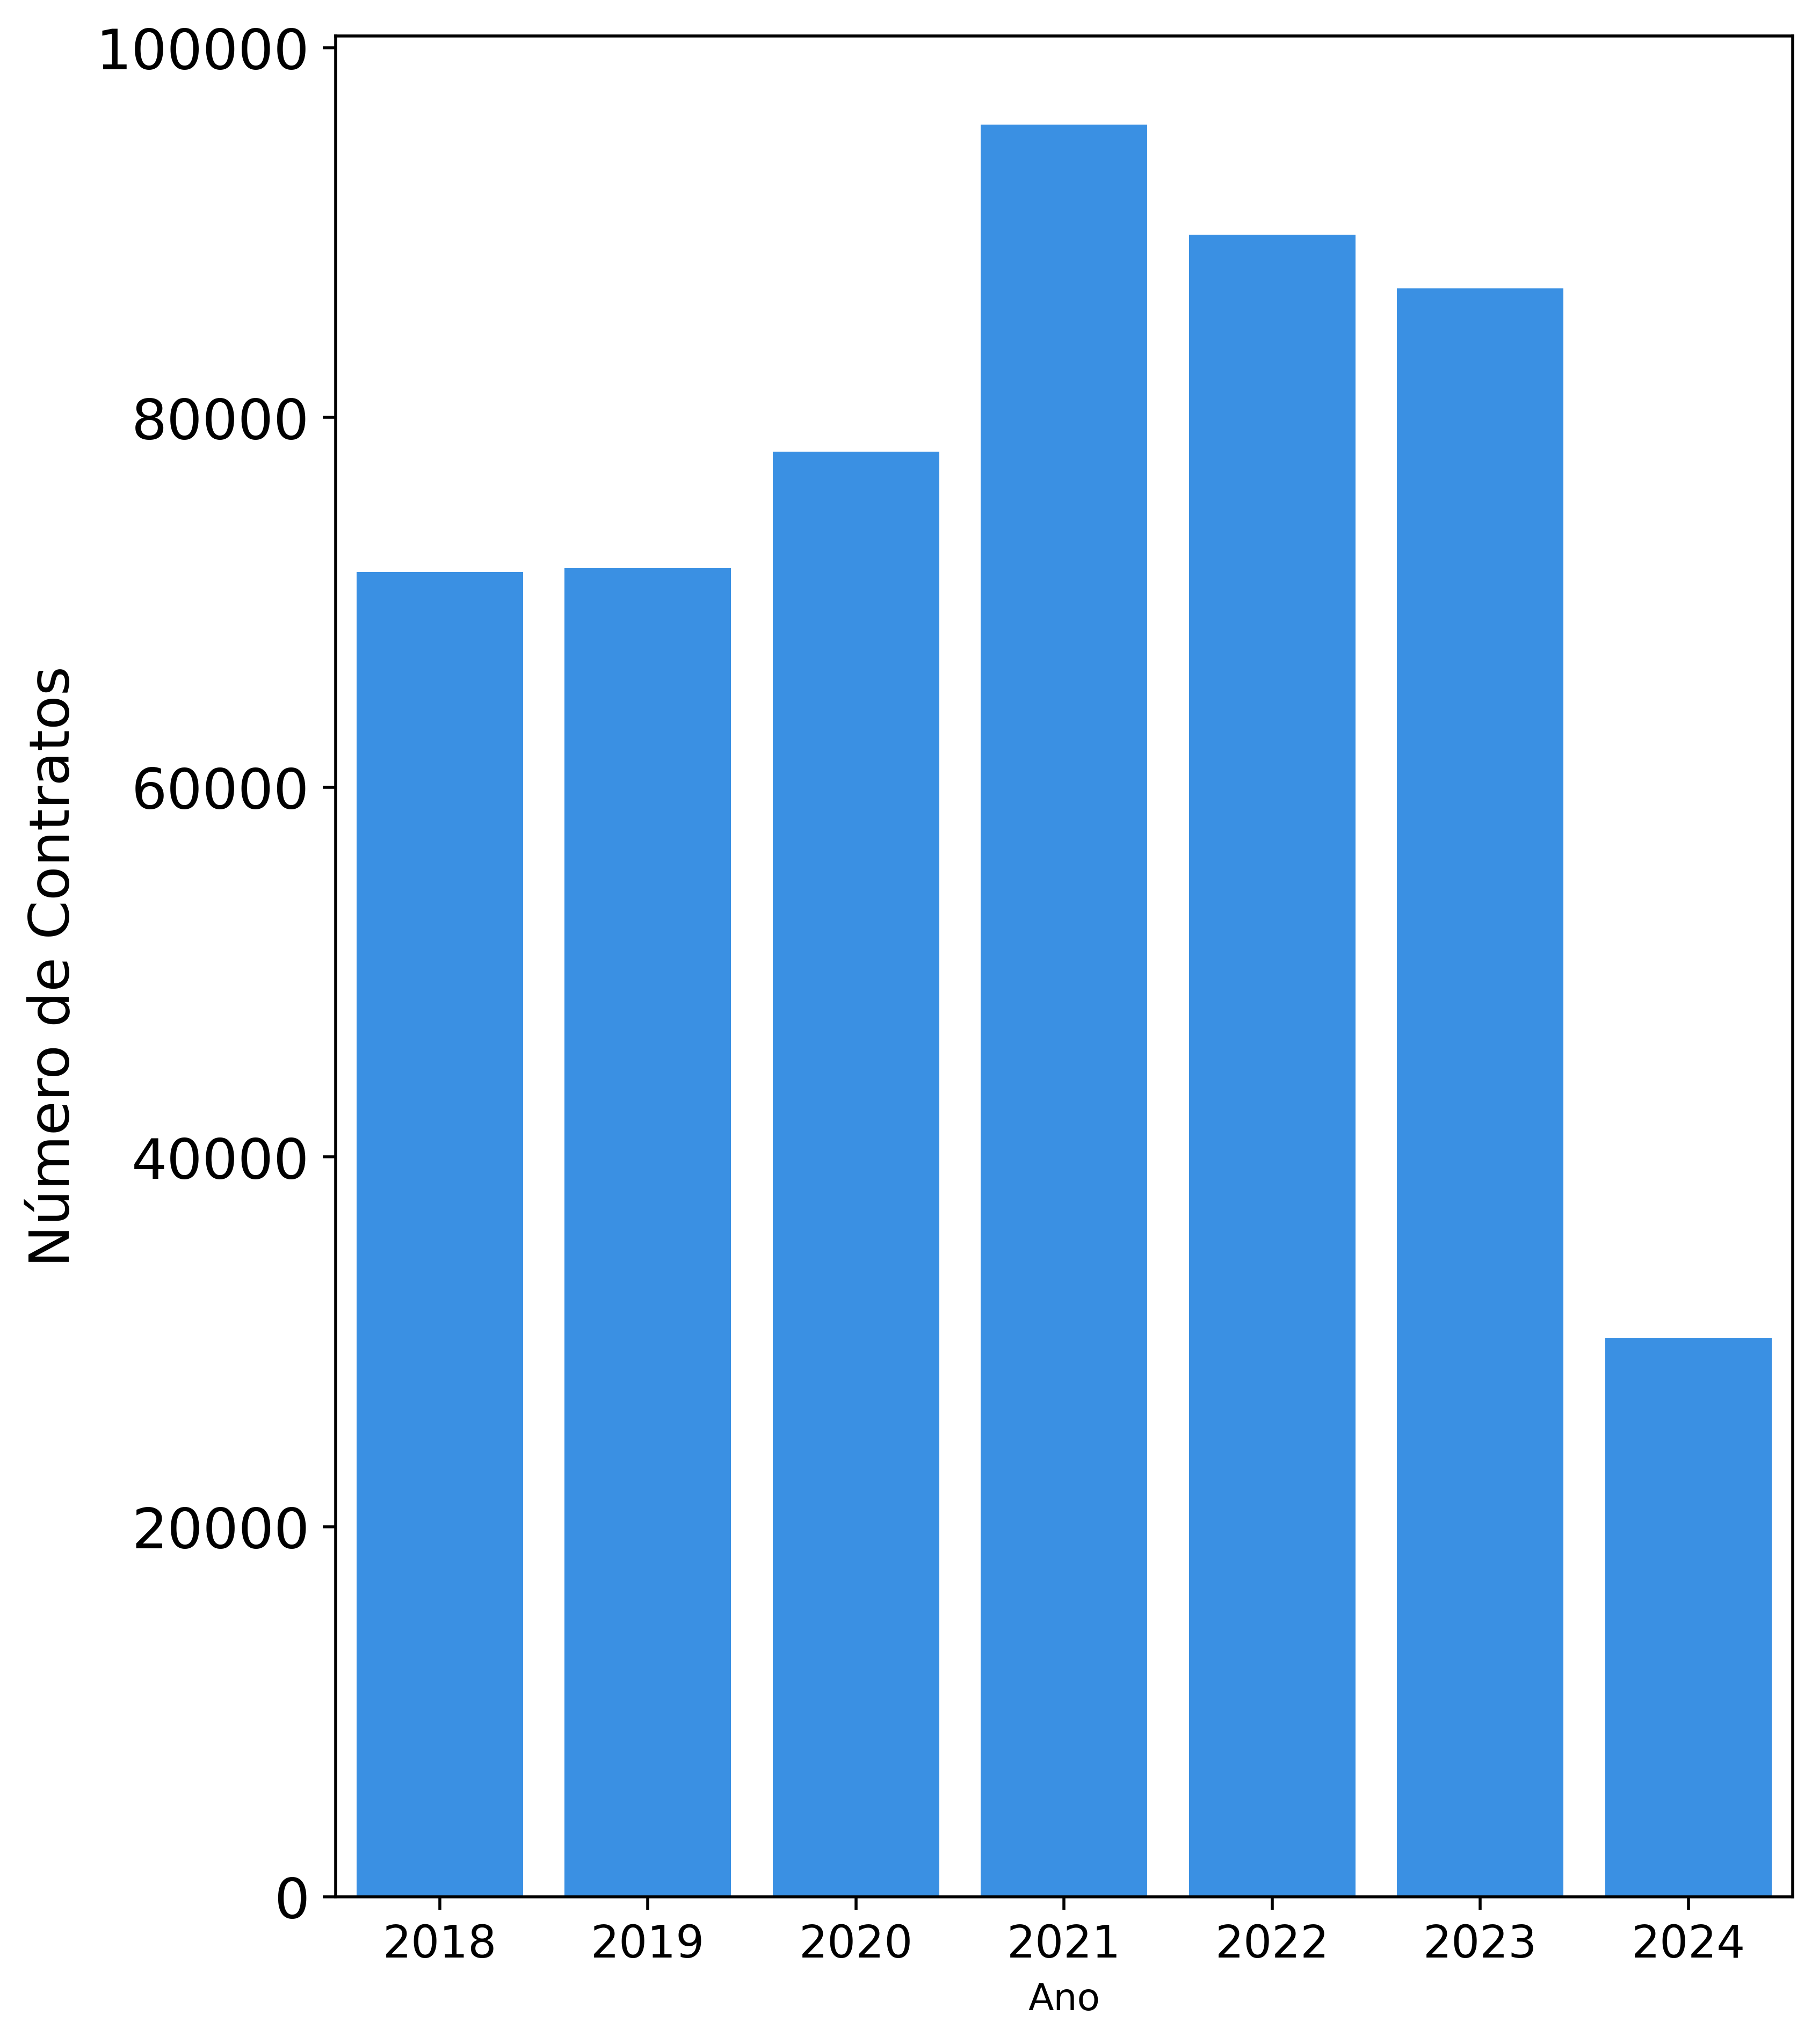
\includegraphics[width=\linewidth]{imagens/adir_nrcontr.png}
		\caption{Número de concursos públicos celebradoss por ano, entre 2018 e 2024}
		\label{fig:precoad1}
	\end{minipage}
	\hfill
	\begin{minipage}{.31\linewidth}
		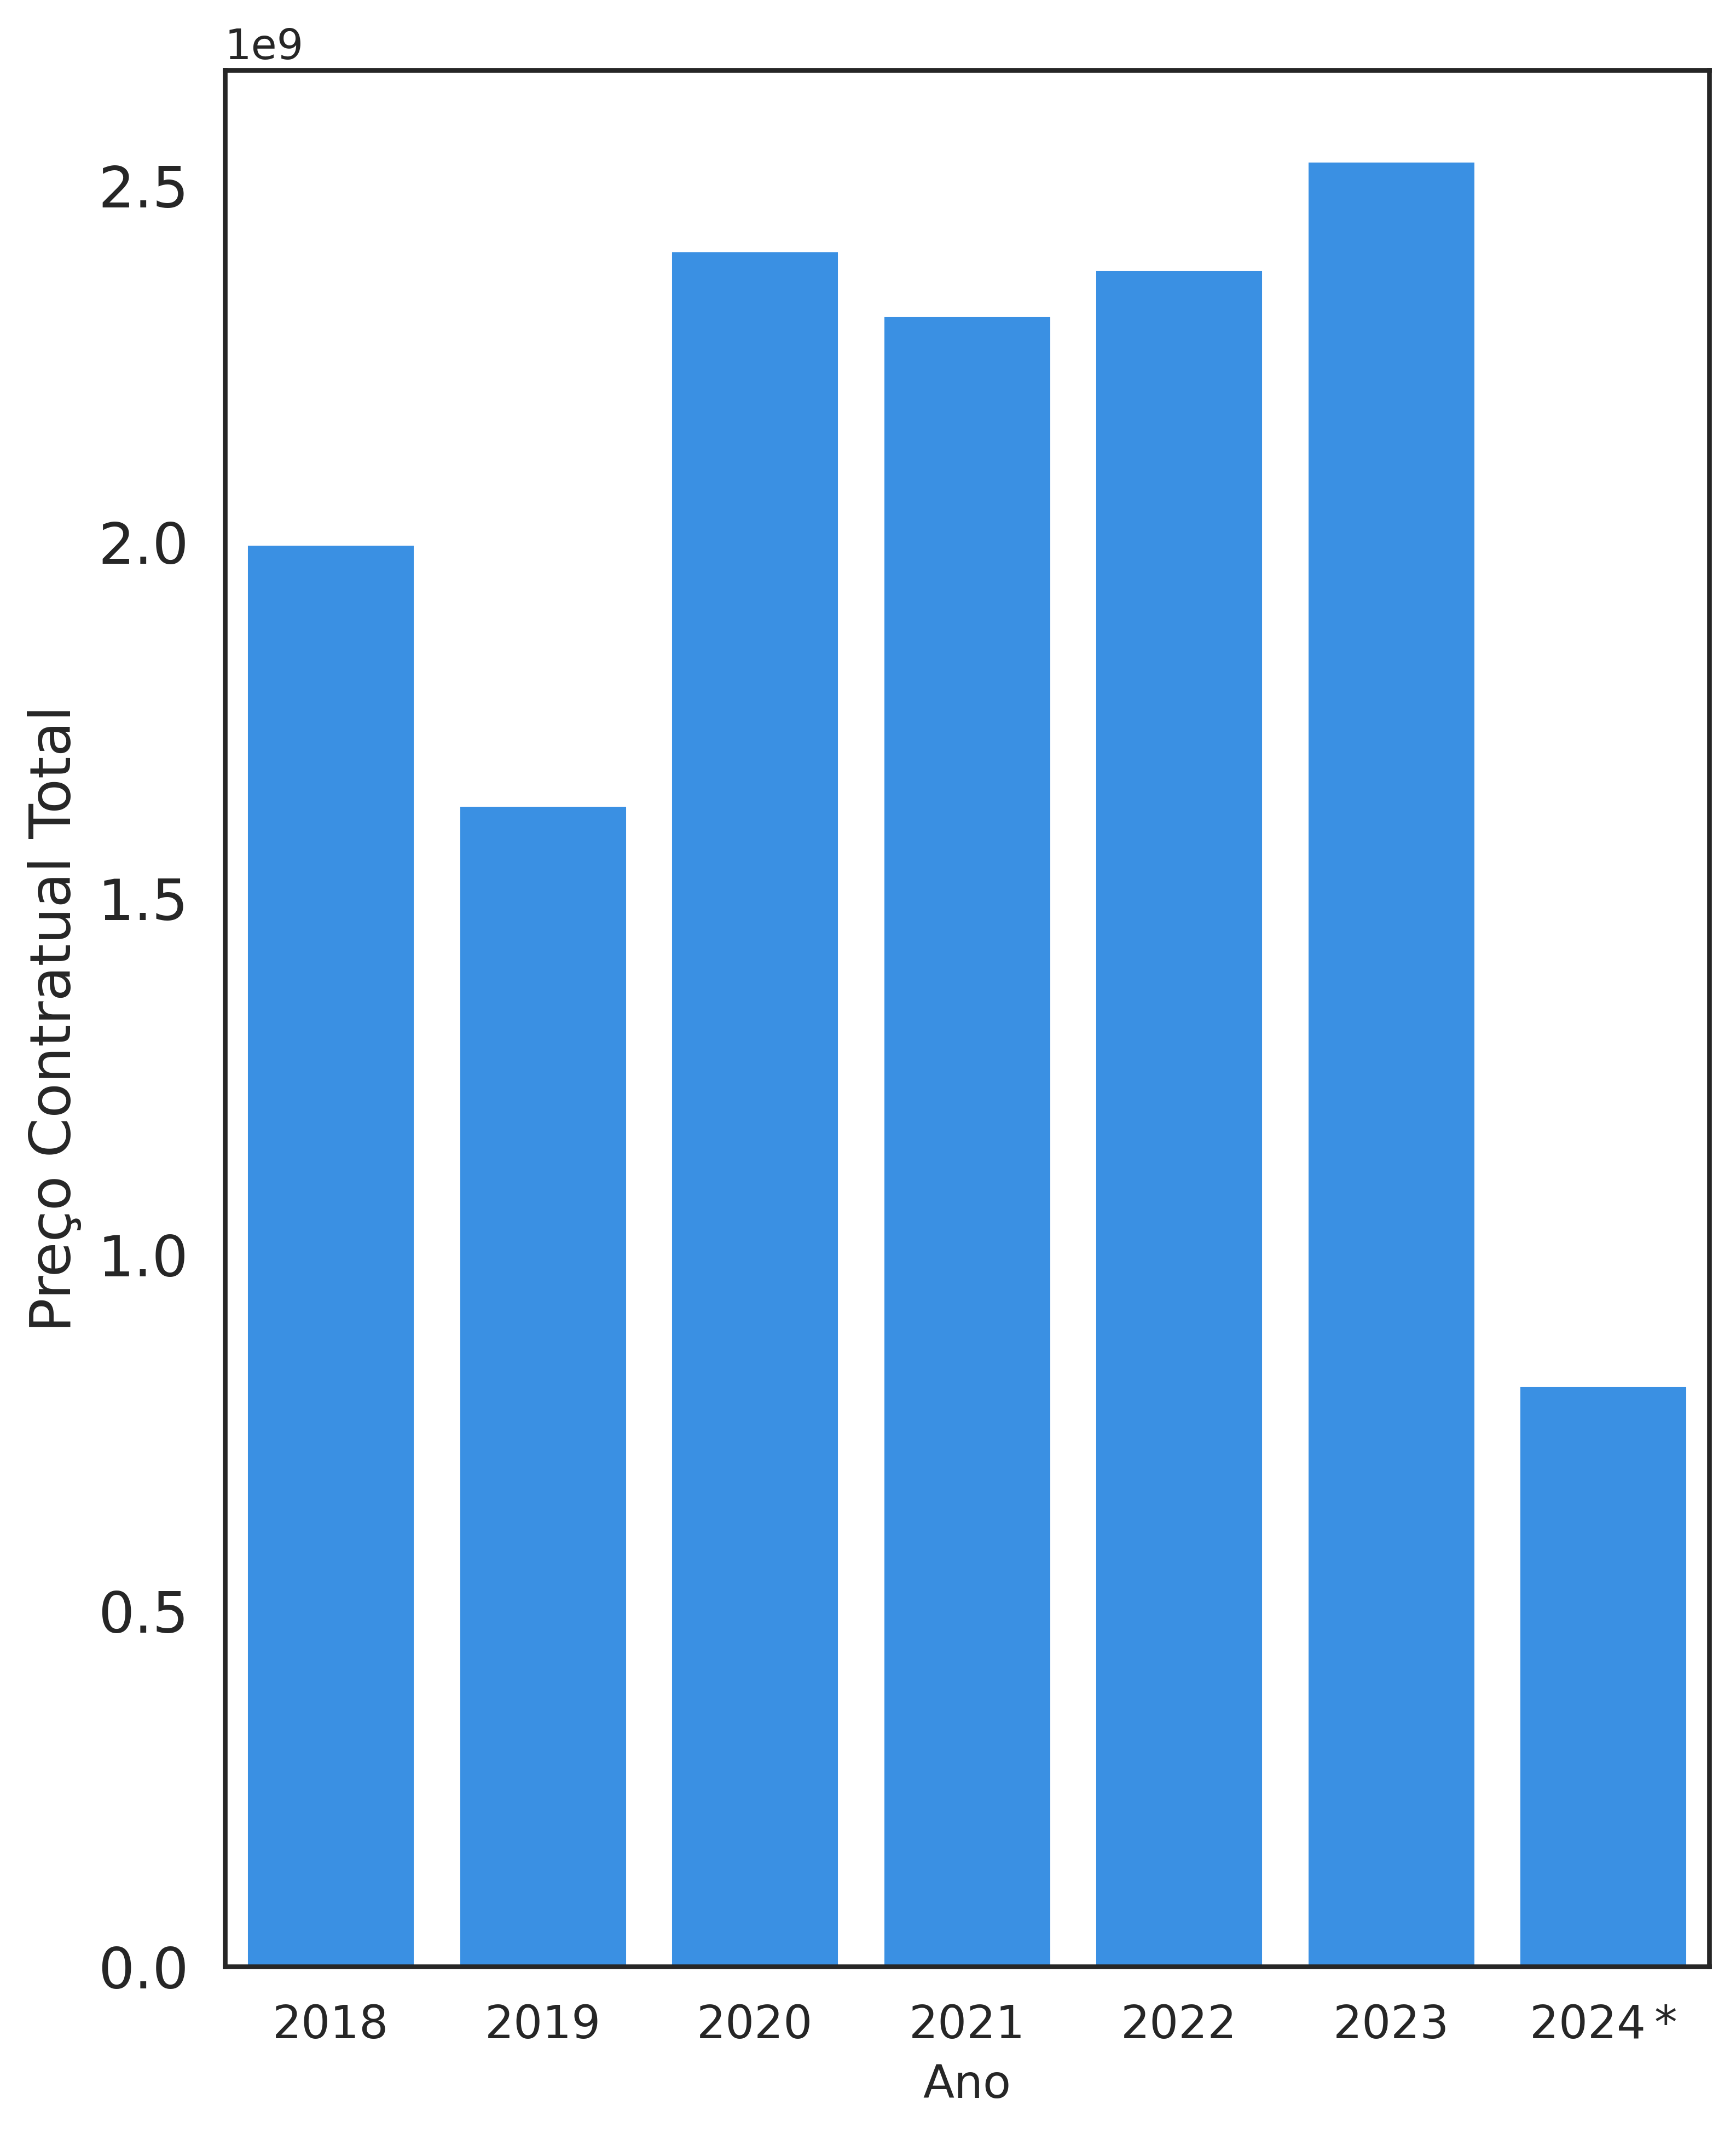
\includegraphics[width=\linewidth]{imagens/adir_price.png}
		\caption{Preço contratual total por ano, entre 2018 e 2024, para concursos públicos}
		\label{fig:precoad2}
	\end{minipage}
\end{figure}



\begin{figure}[H]
	\begin{minipage}[t]{.55\textwidth}
		\centering
		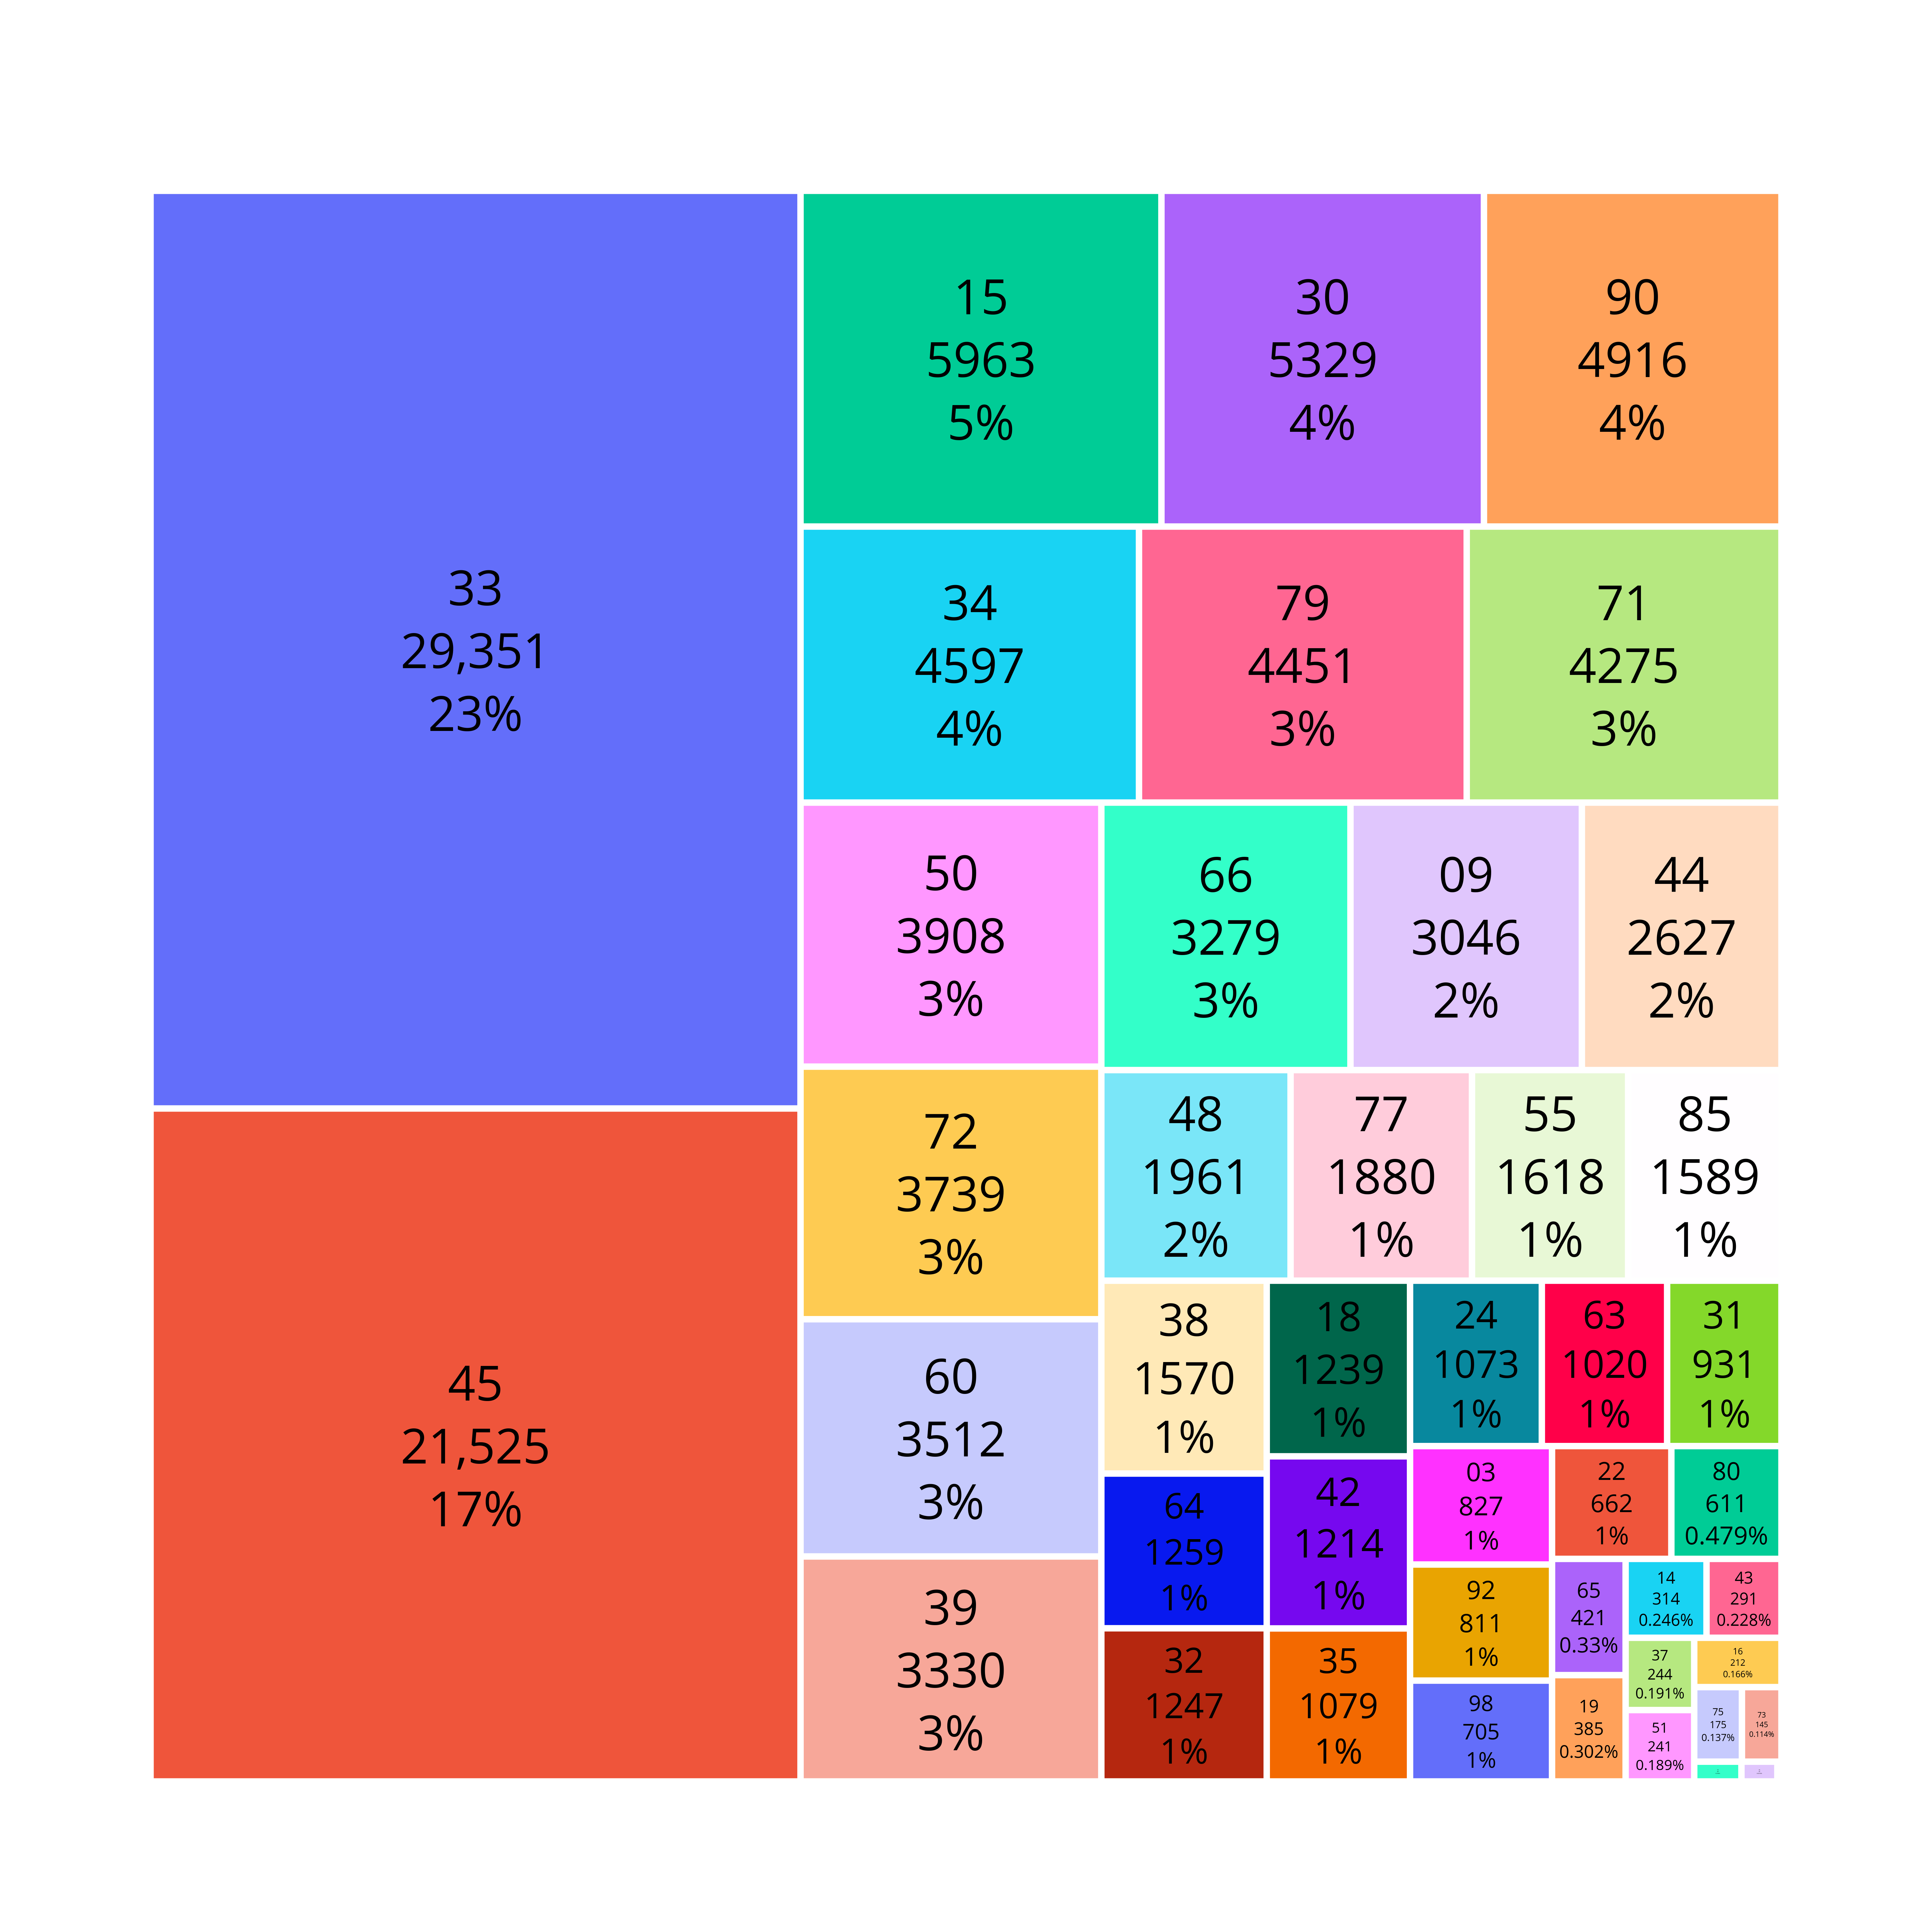
\includegraphics[width=\textwidth]{imagens/treemap_cpub.png}
		\caption{Distribuição do número de concursos públicos por divisão de CPV}
	\end{minipage}
	\begin{minipage}[t]{.55\textwidth}
		\centering
		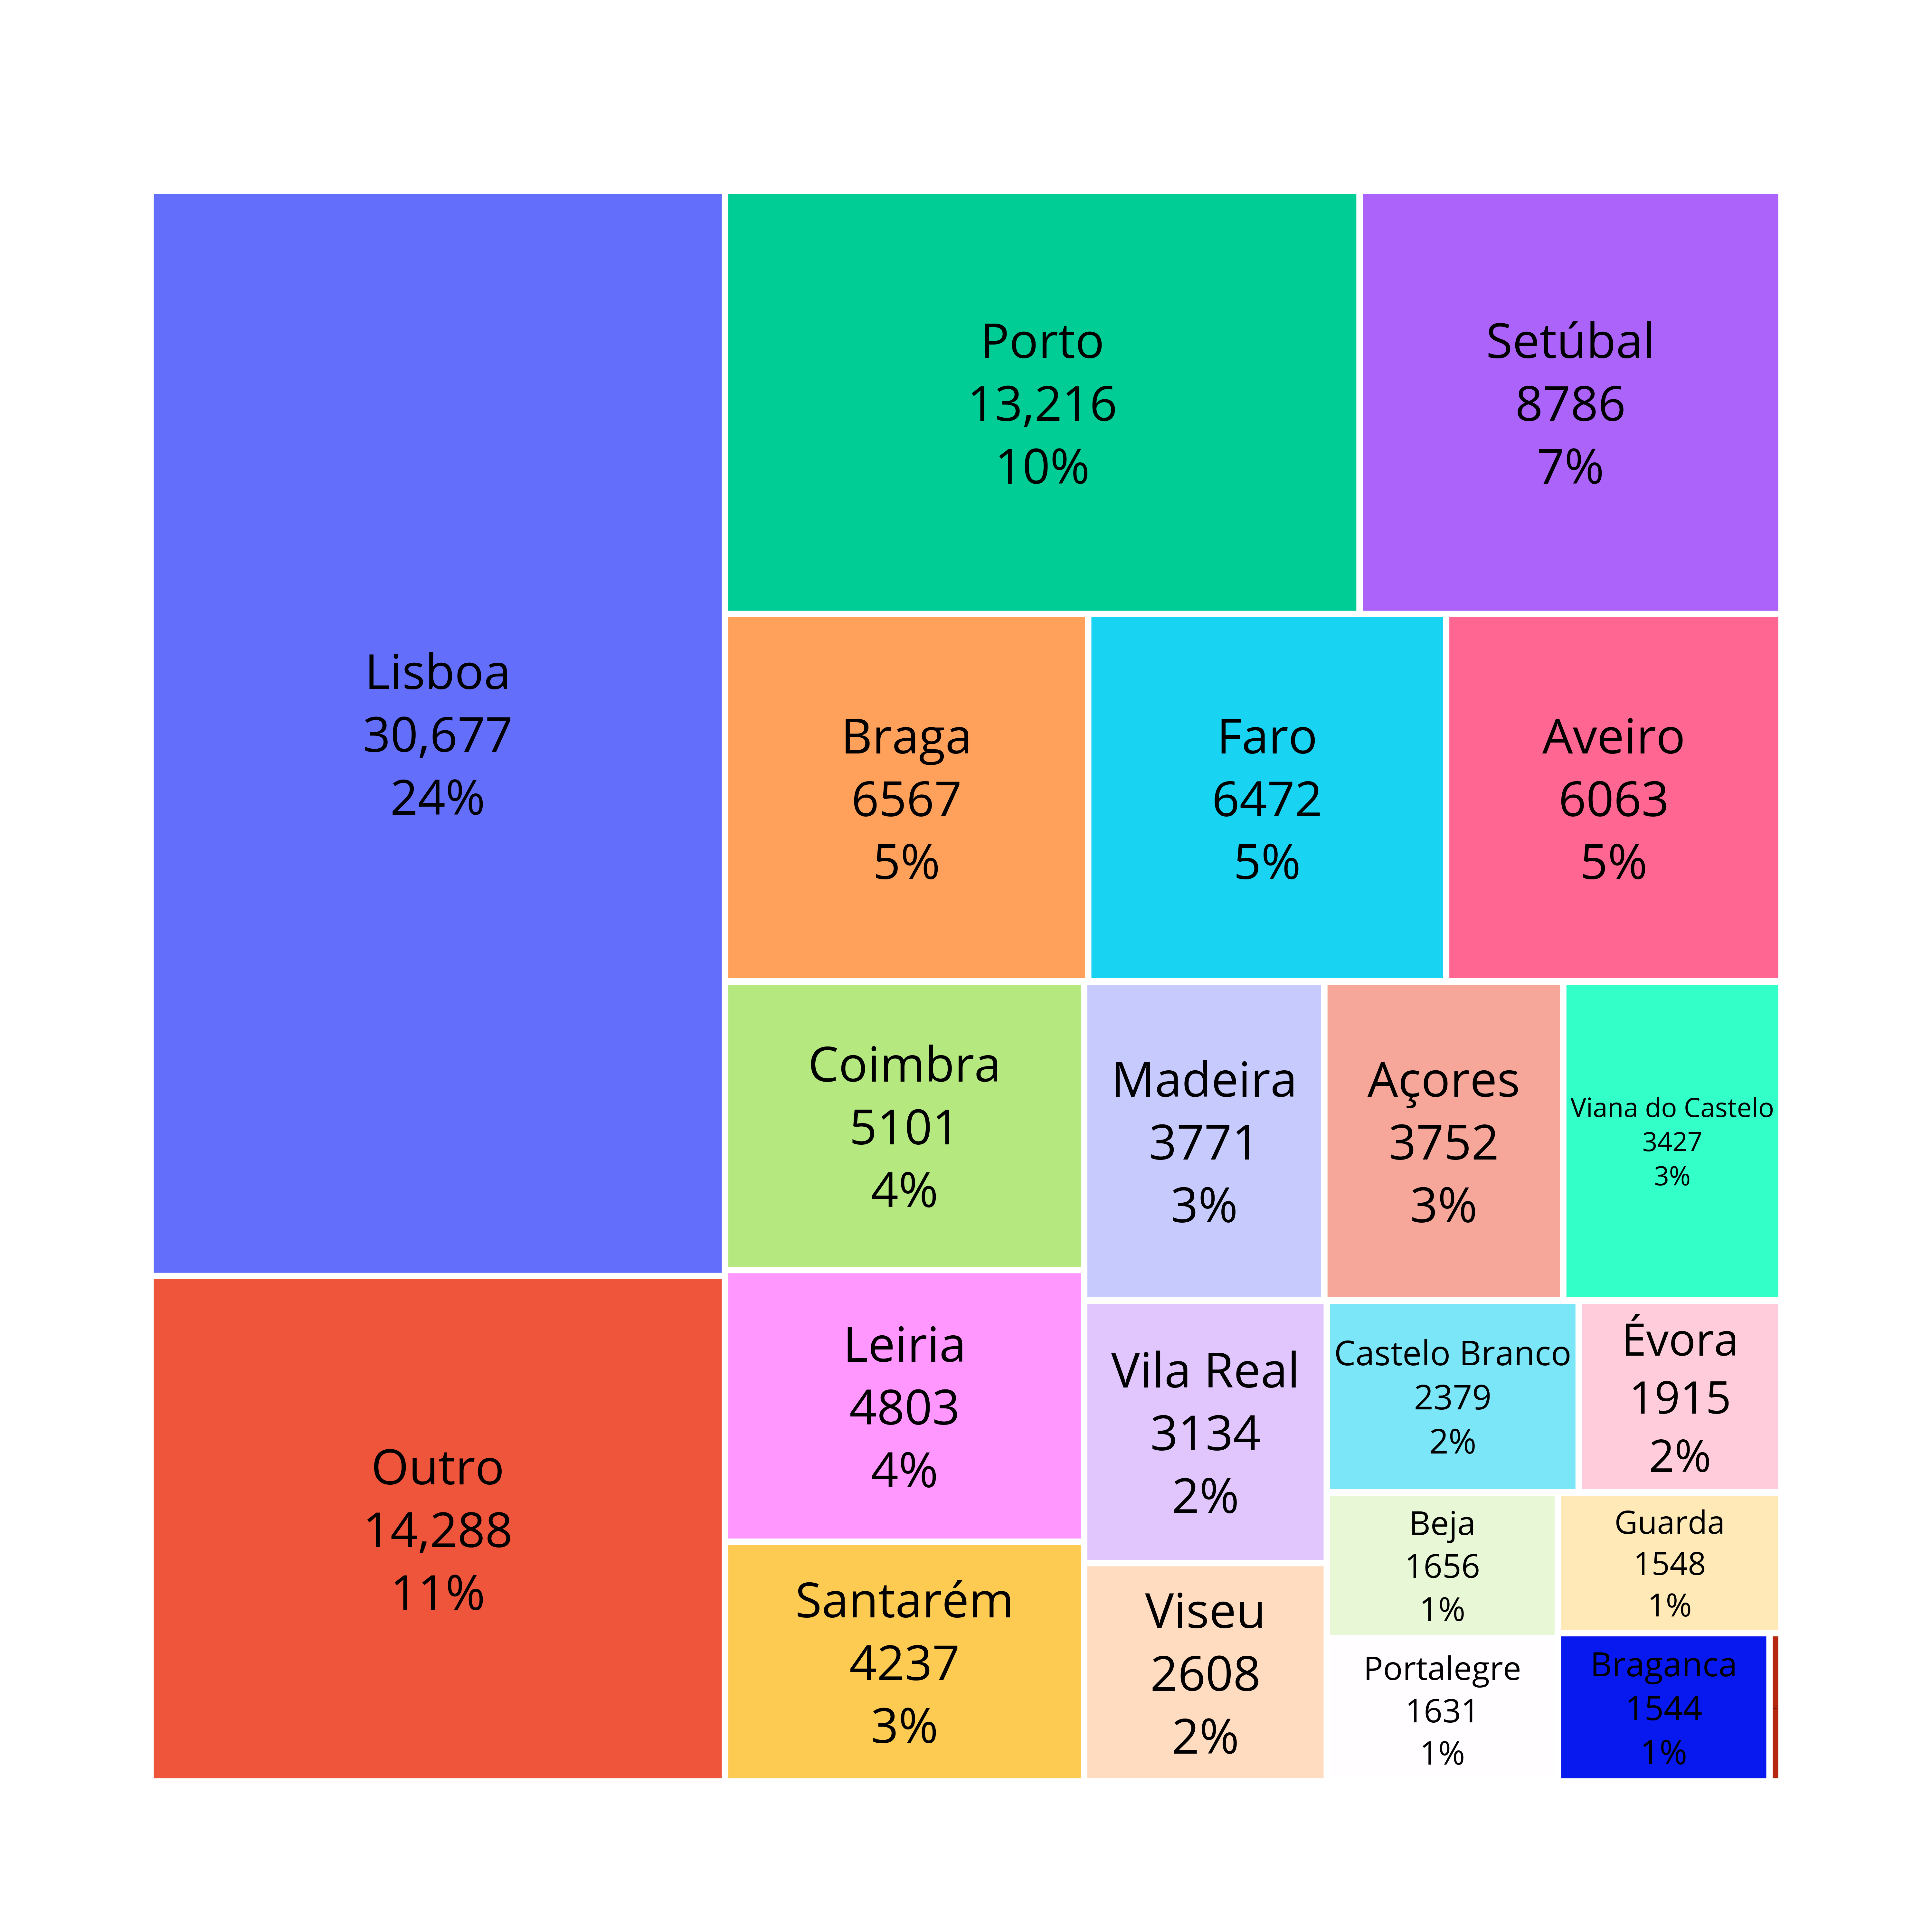
\includegraphics[width=\textwidth]{imagens/treemap_cpub_distritos.png}
		\caption{Distribuição do número de contratos públicos por distrito}
	\end{minipage}
	
	\medskip
	
	\begin{minipage}[t]{.55\textwidth}
		\centering
		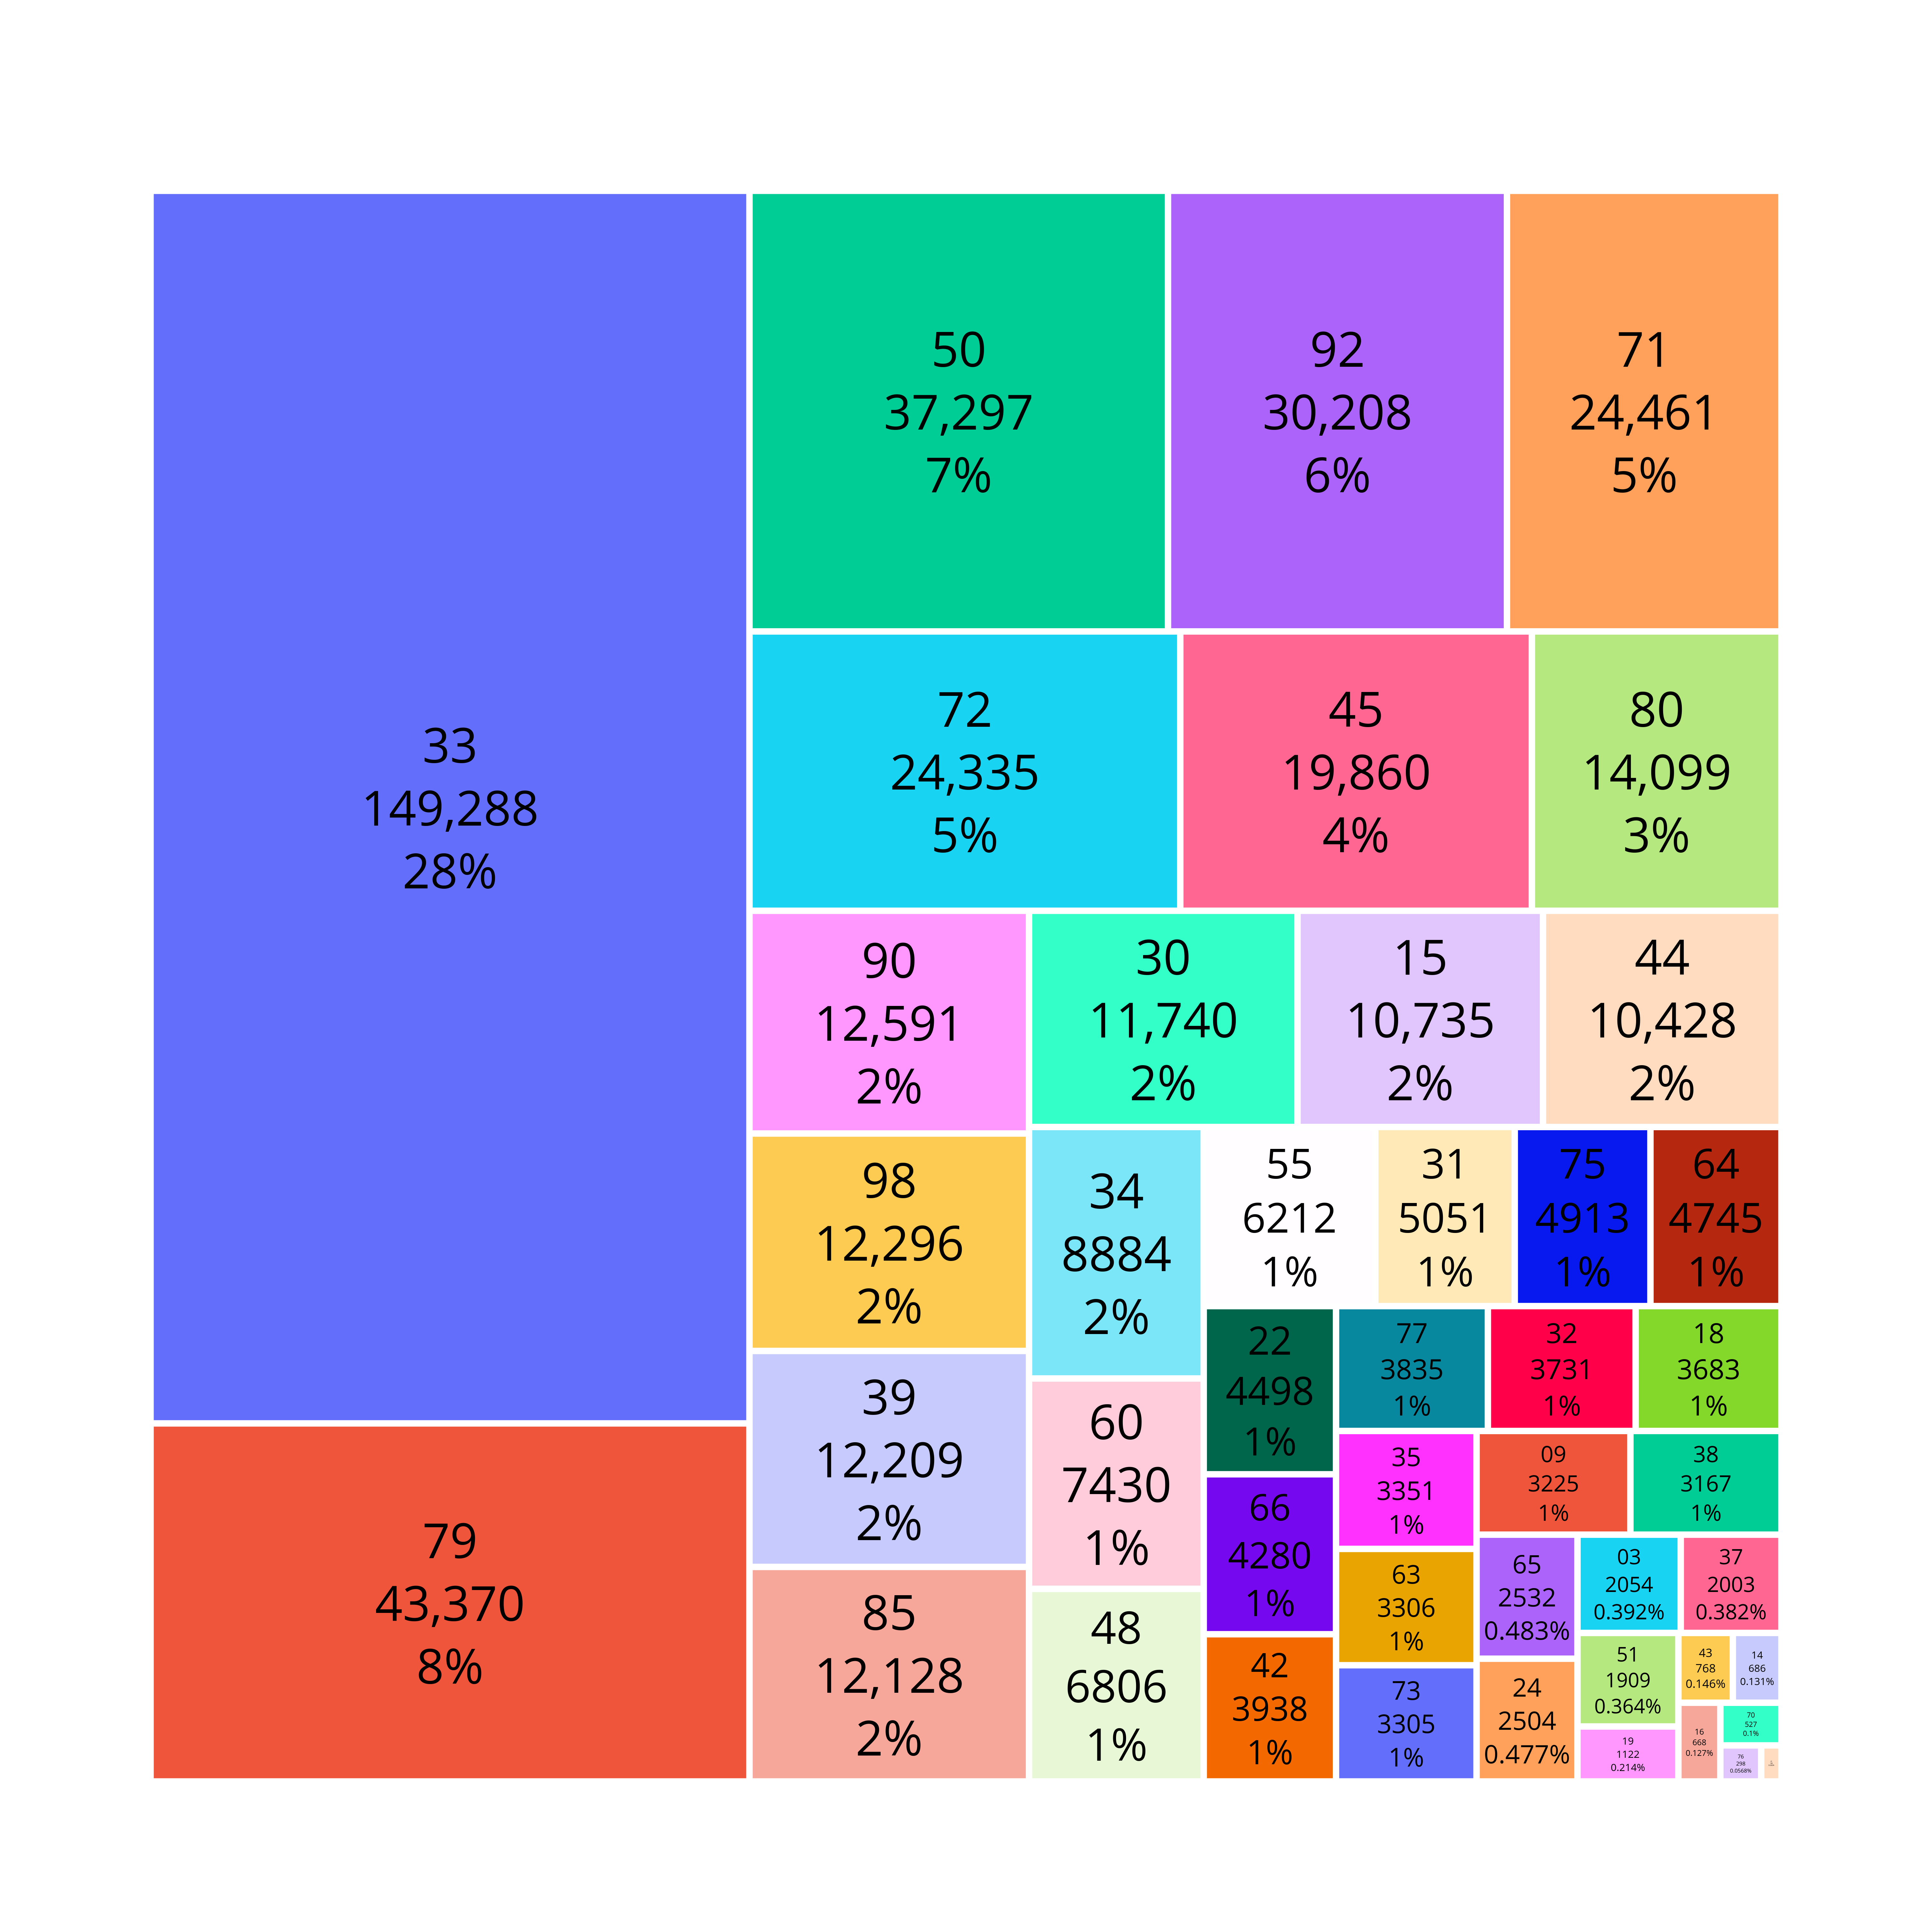
\includegraphics[width=\textwidth]{imagens/treemap_contratos_adir.png}
		\caption{Distribuição do número de ajustes diretos em regime geral por divisão de CPV}
	\end{minipage}
	\begin{minipage}[t]{.55\textwidth}
		\centering
		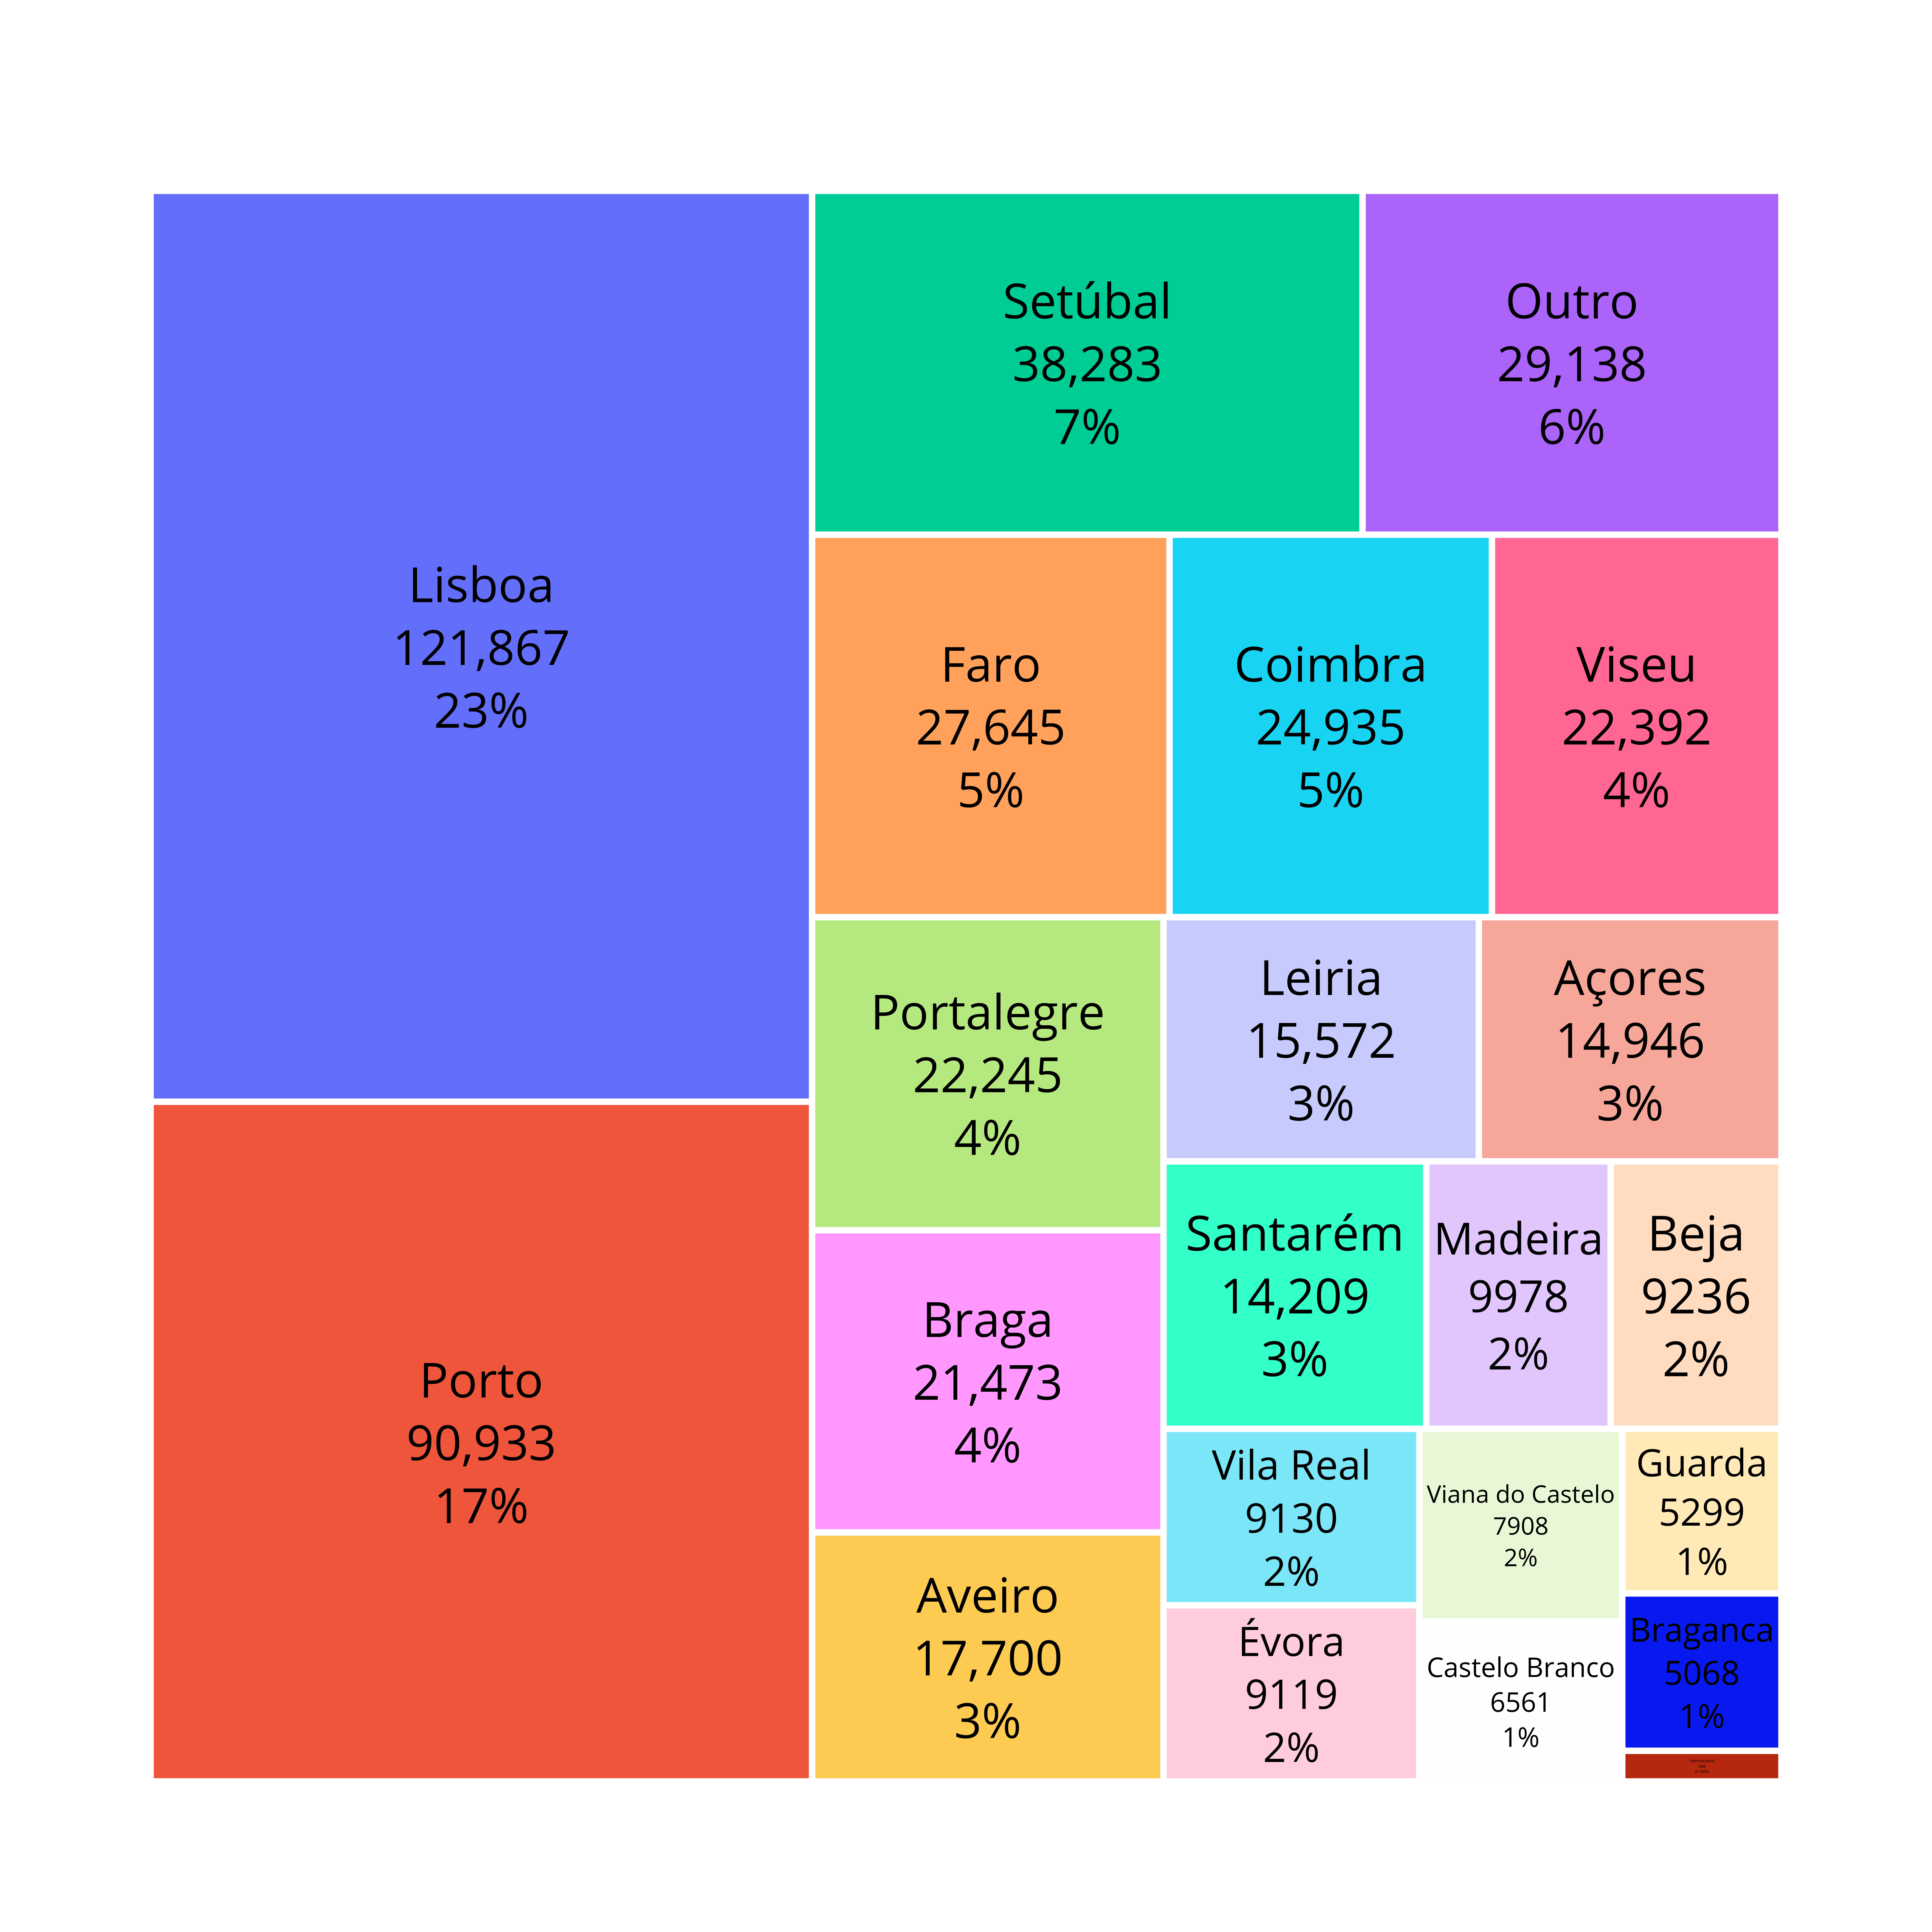
\includegraphics[width=\textwidth]{imagens/treemap_distritos_adir.png}
		\caption{Distribuição do número de ajustes diretos em regime geral por distrito}
	\end{minipage}
\end{figure}
























































%\subsection{Exemplo ilustrativo: Contratos referentes à área da saúde}
%
%\begin{figure}[H]
%	\begin{minipage}{0.33\linewidth}
%		%\centering  % redundant
%		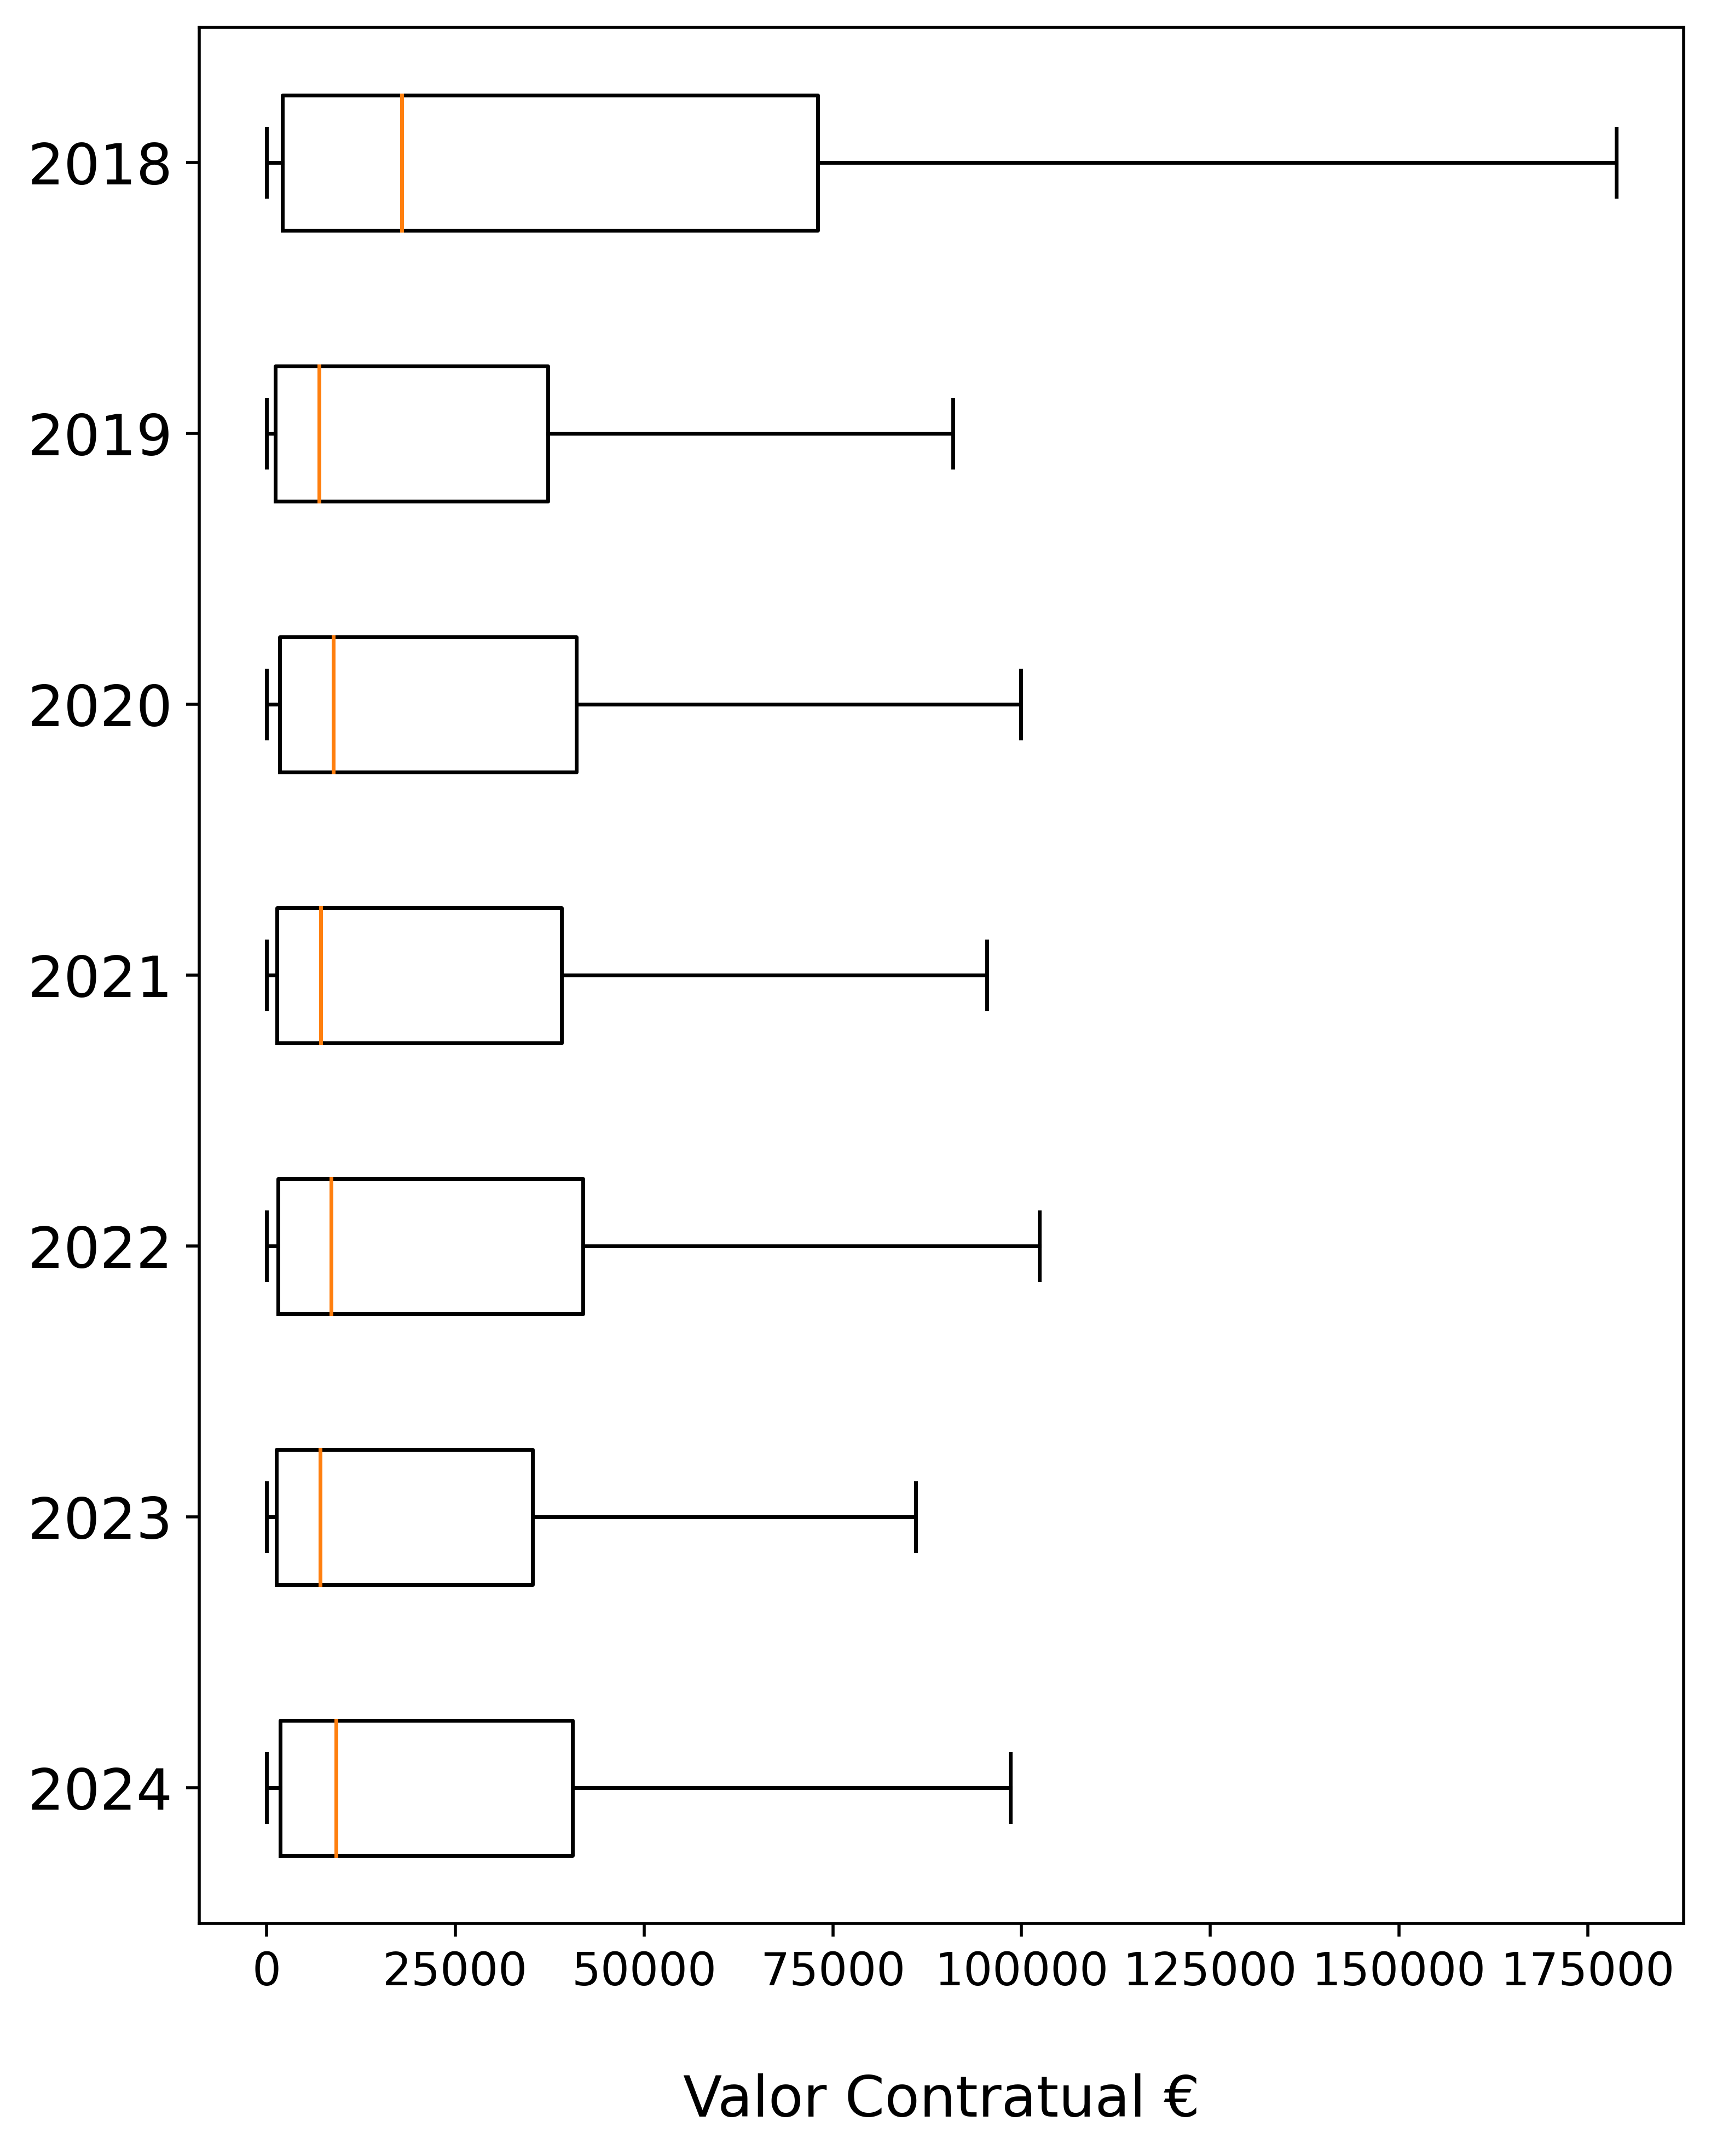
\includegraphics[width=\textwidth]{imagens/cp_anos_33_v1.png}
%		\caption{Boxplot dos preços contratuais para concursos públicos referentes à área da saúde desde 2018 até 2024}
%	\end{minipage}%
%	\hfill% not: "\hspace{0.5cm}"
%	\begin{minipage}{0.33\linewidth}
%		%\centering  % redundant
%		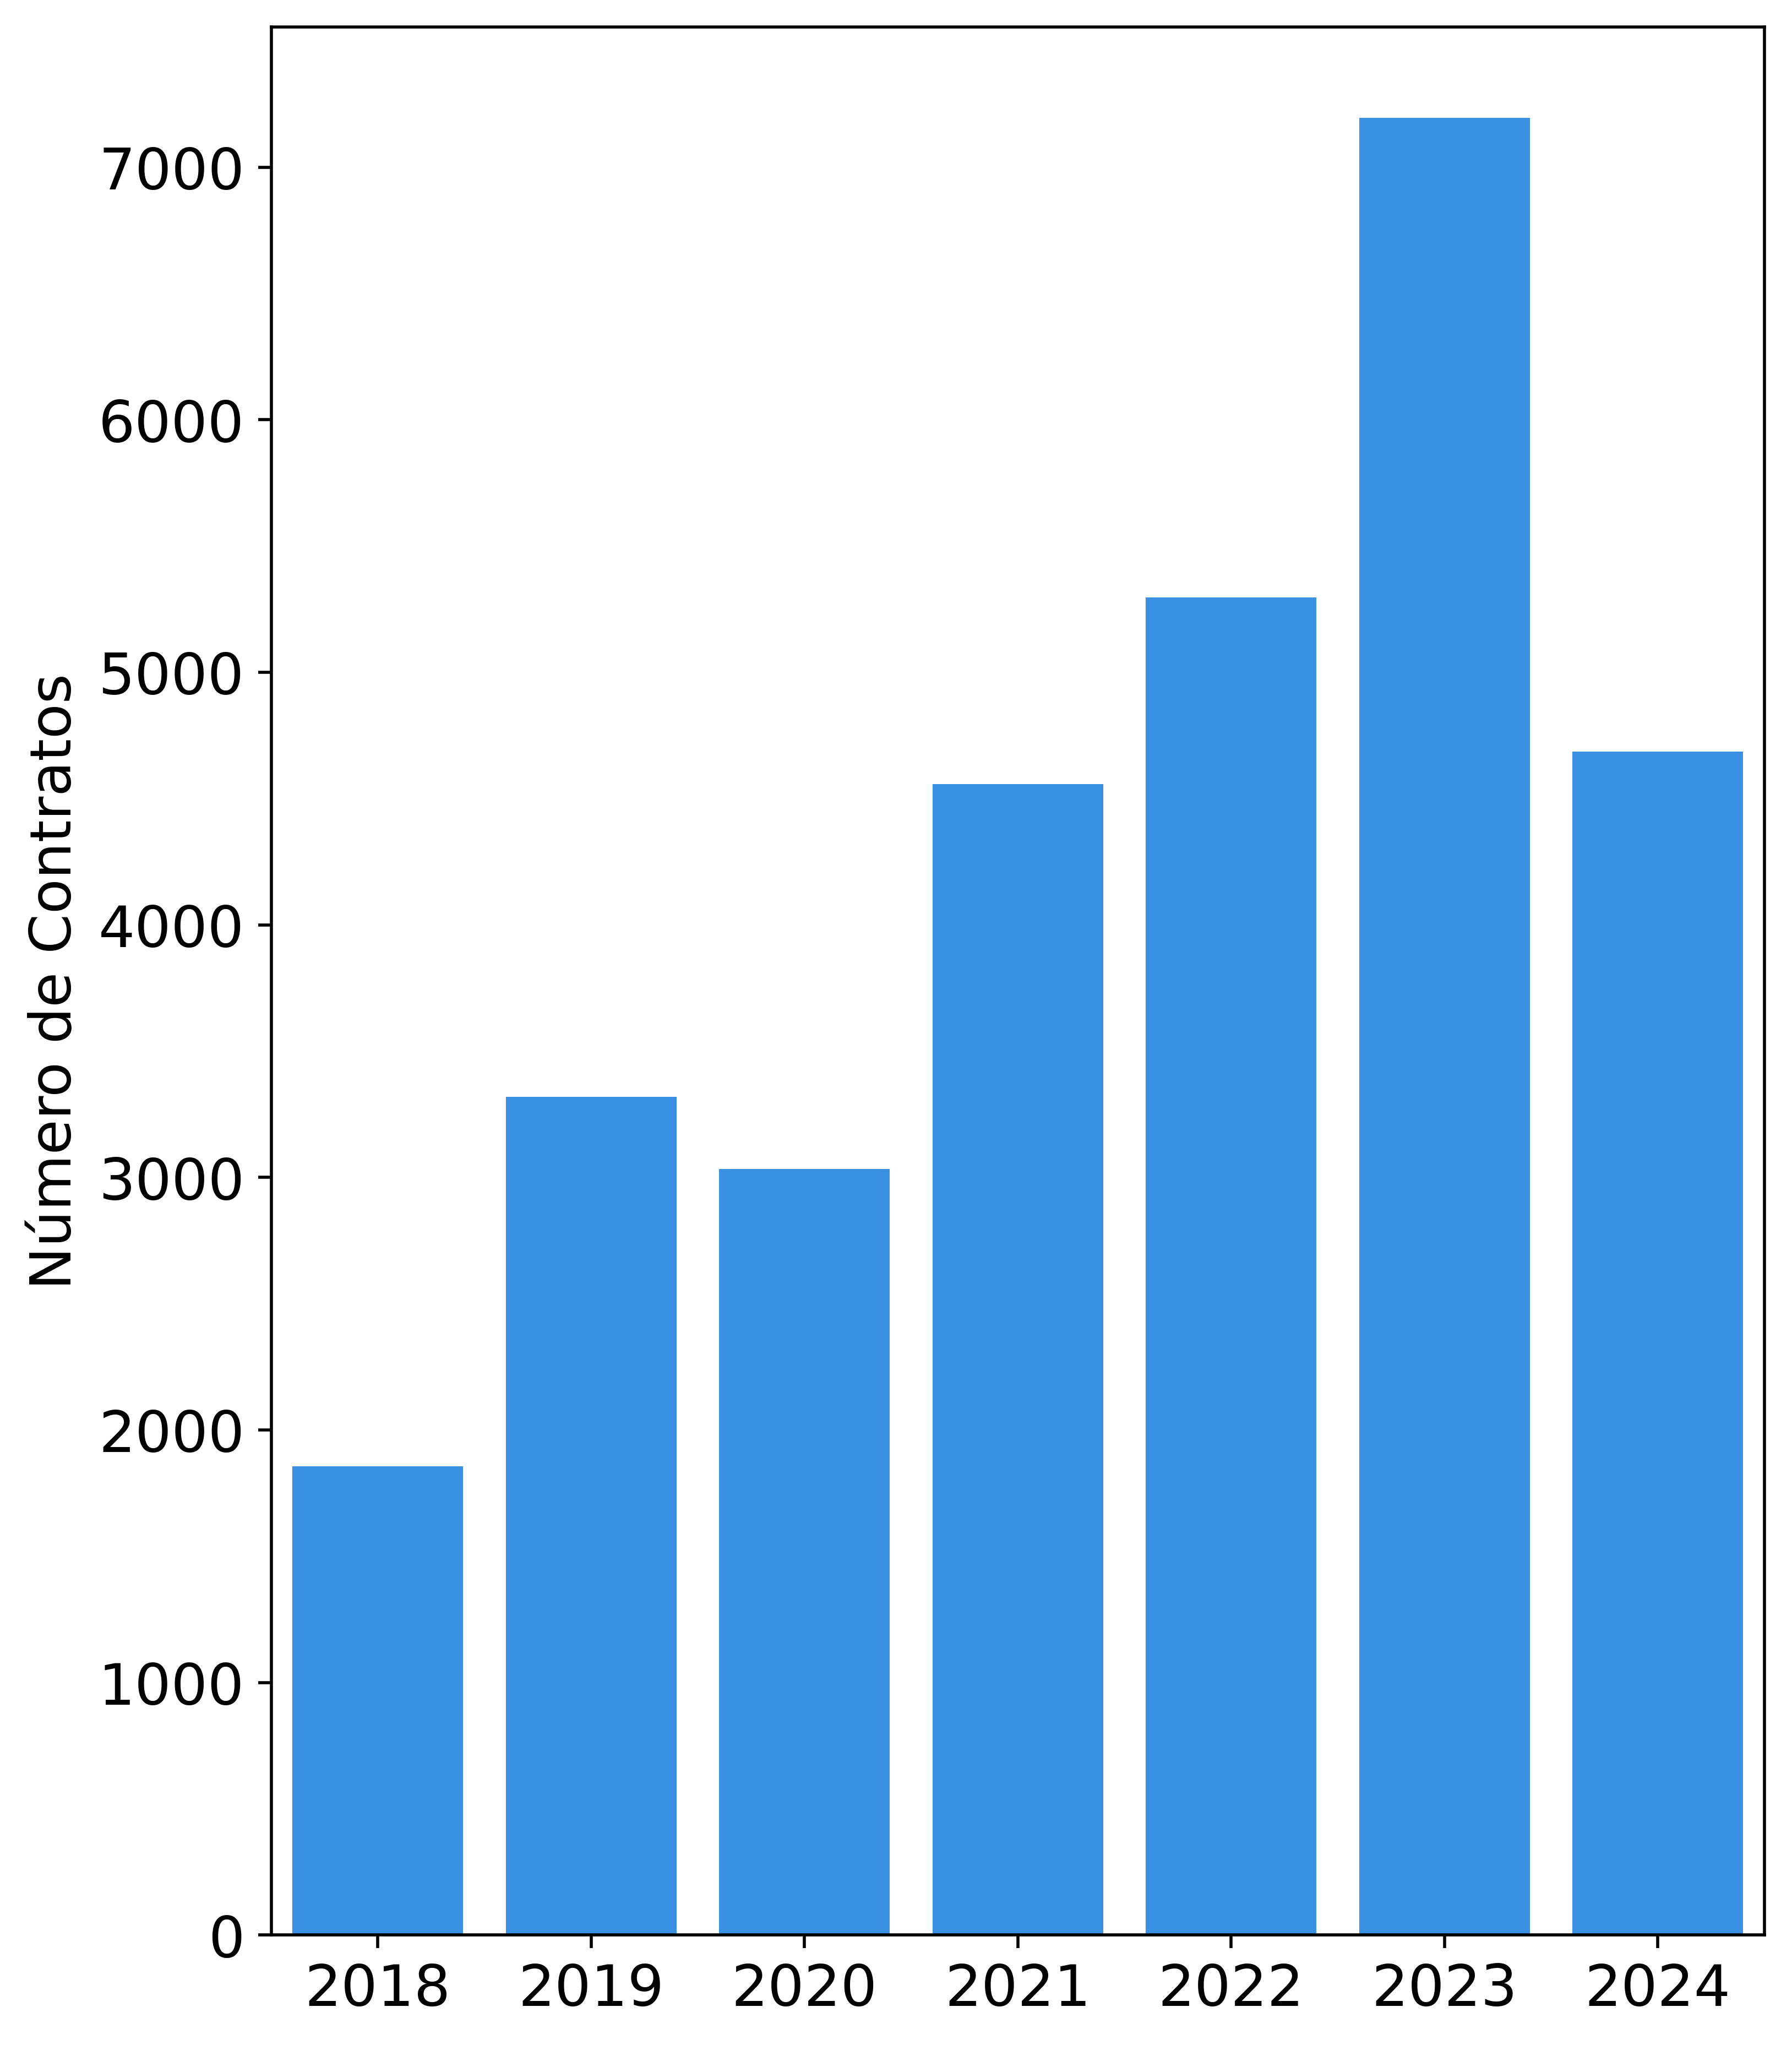
\includegraphics[width=\textwidth]{imagens/cp_anos_33_v2.png}
%		\caption{Número de concursos públicos celebrados referentes à área da saúde desde 2018 até 2024}
%	\end{minipage}%
%	\hfill% not: "\hspace{0.5cm}"
%	\begin{minipage}{0.33\linewidth}
%		%\centering  % redundant
%		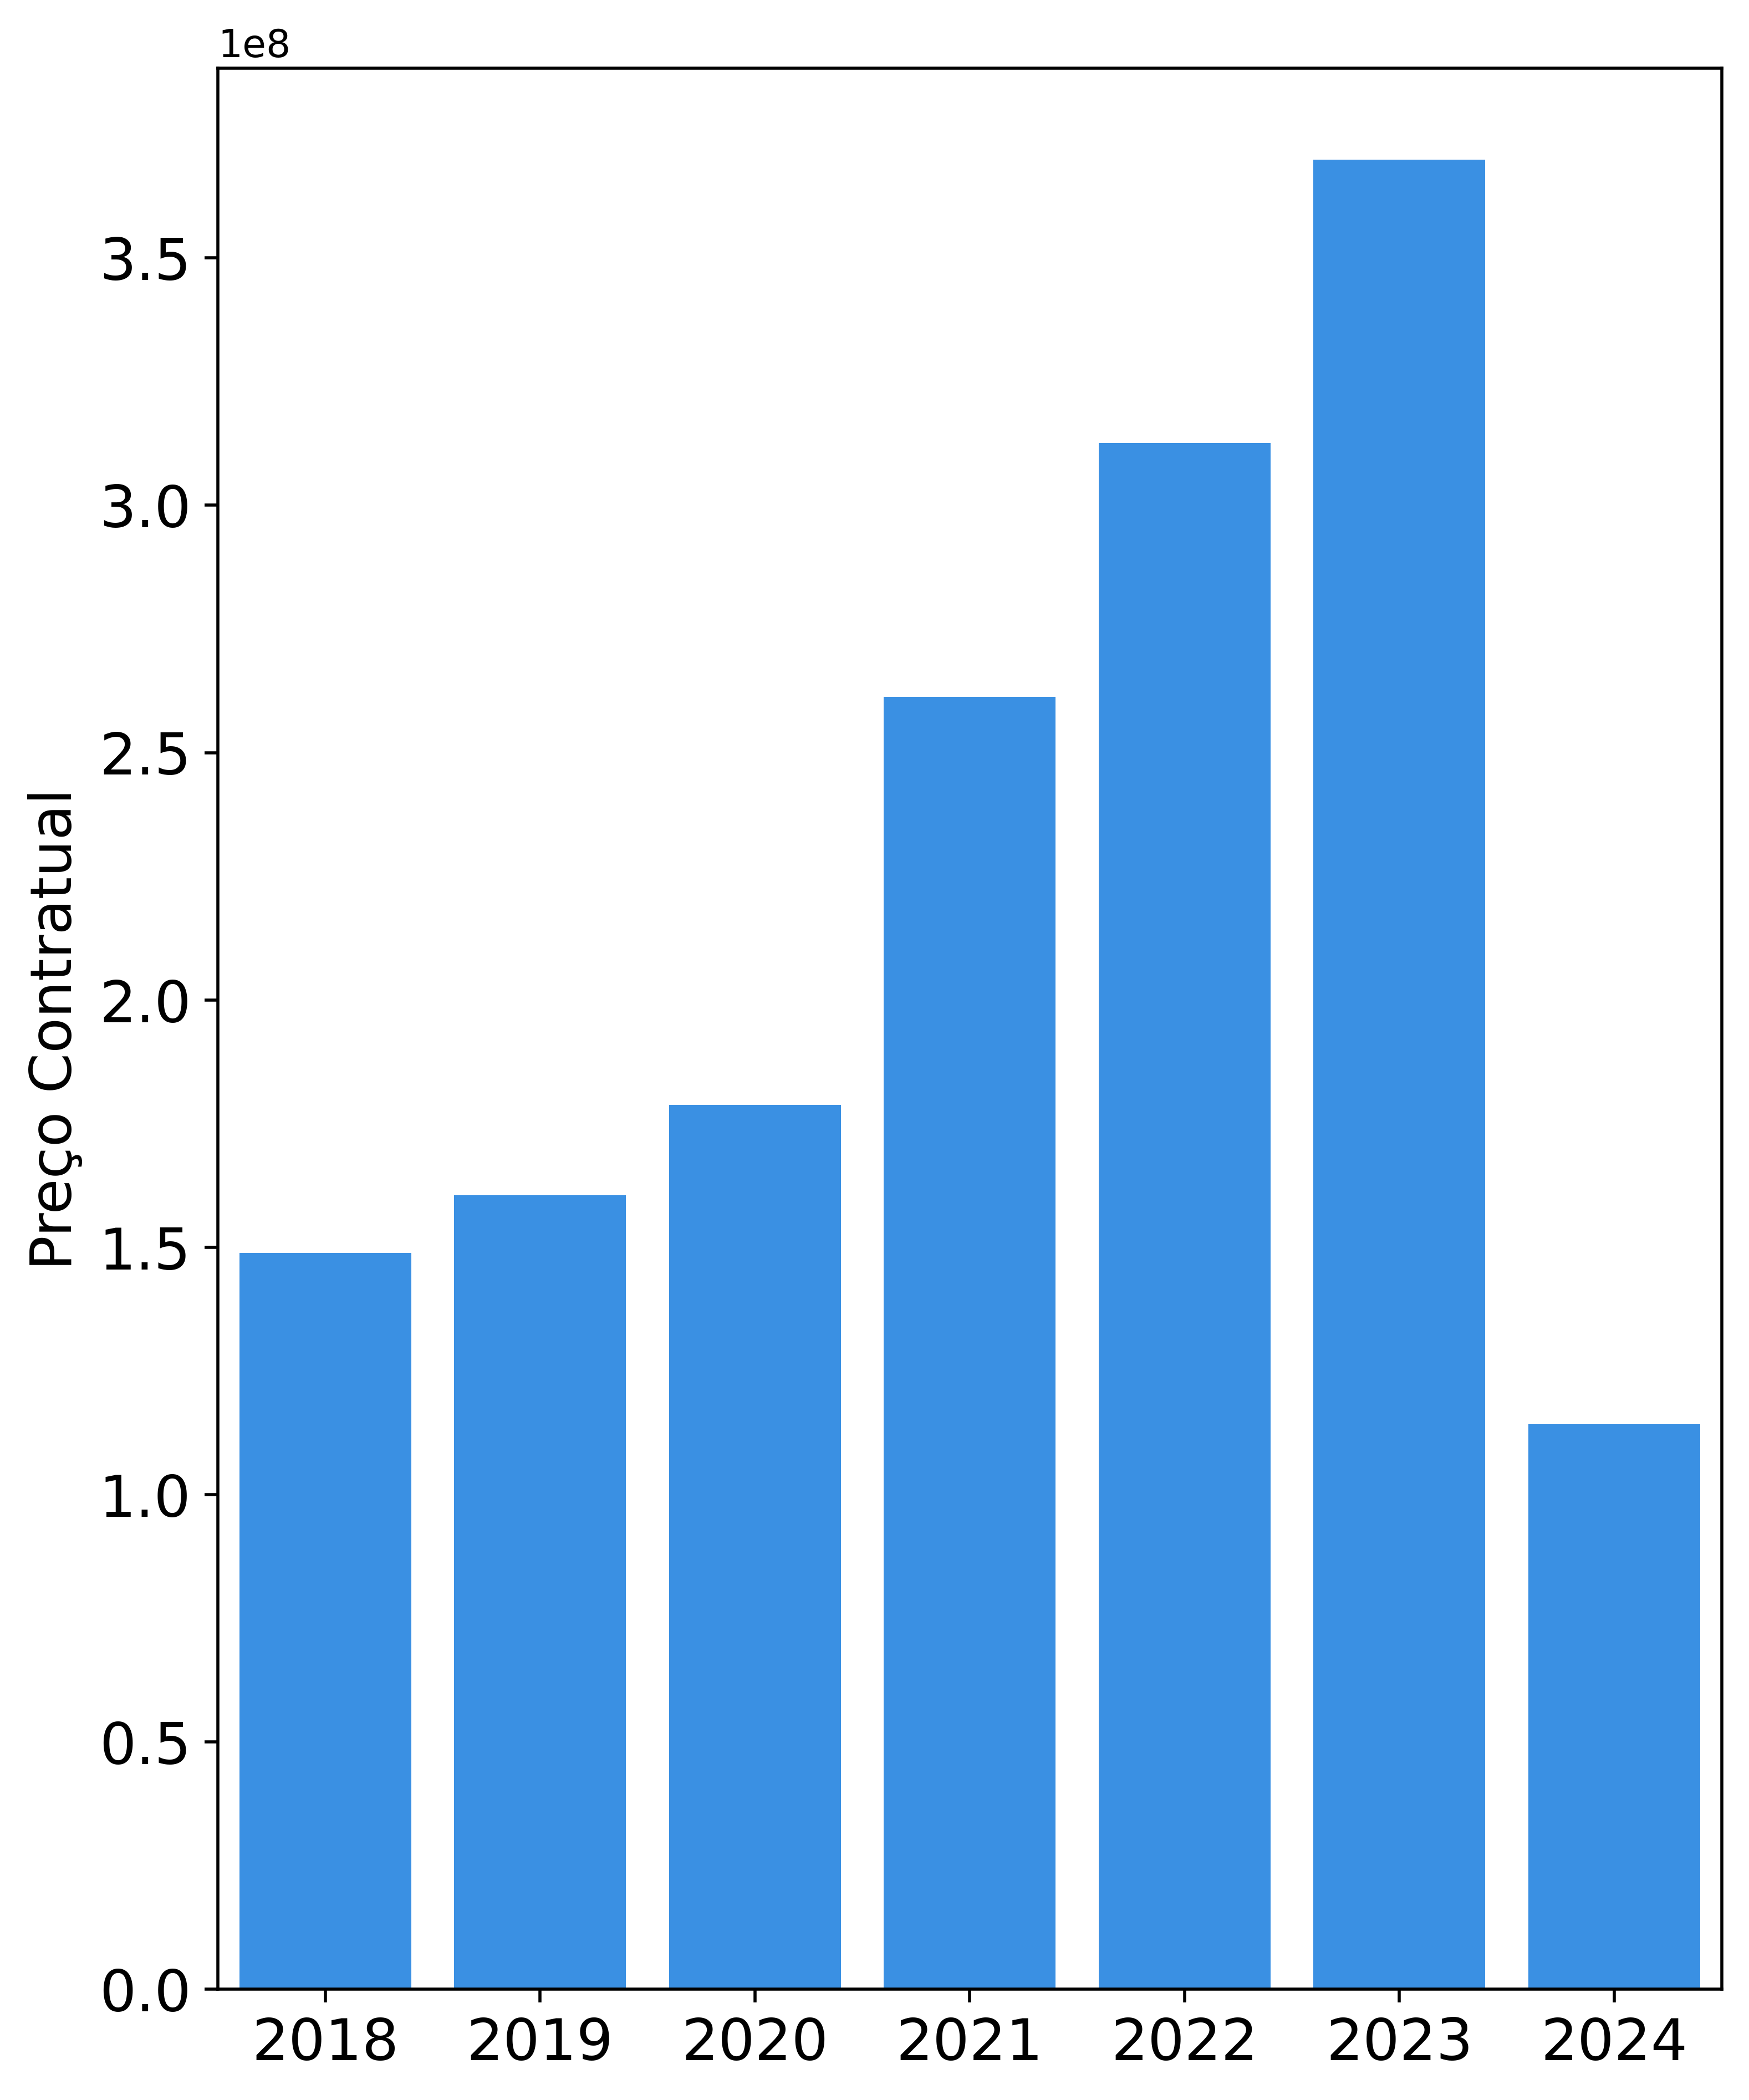
\includegraphics[width=\textwidth]{imagens/cp_anos_33_v3.png}
%		\caption{Montante total adjudicada a contratos públicos celebrados referentes à área da saúde desde 2018 até 2024}
%	\end{minipage}
%\end{figure}
%
%
%
%\begin{figure}[H]
%	\begin{minipage}{0.33\linewidth}
%		%\centering  % redundant
%		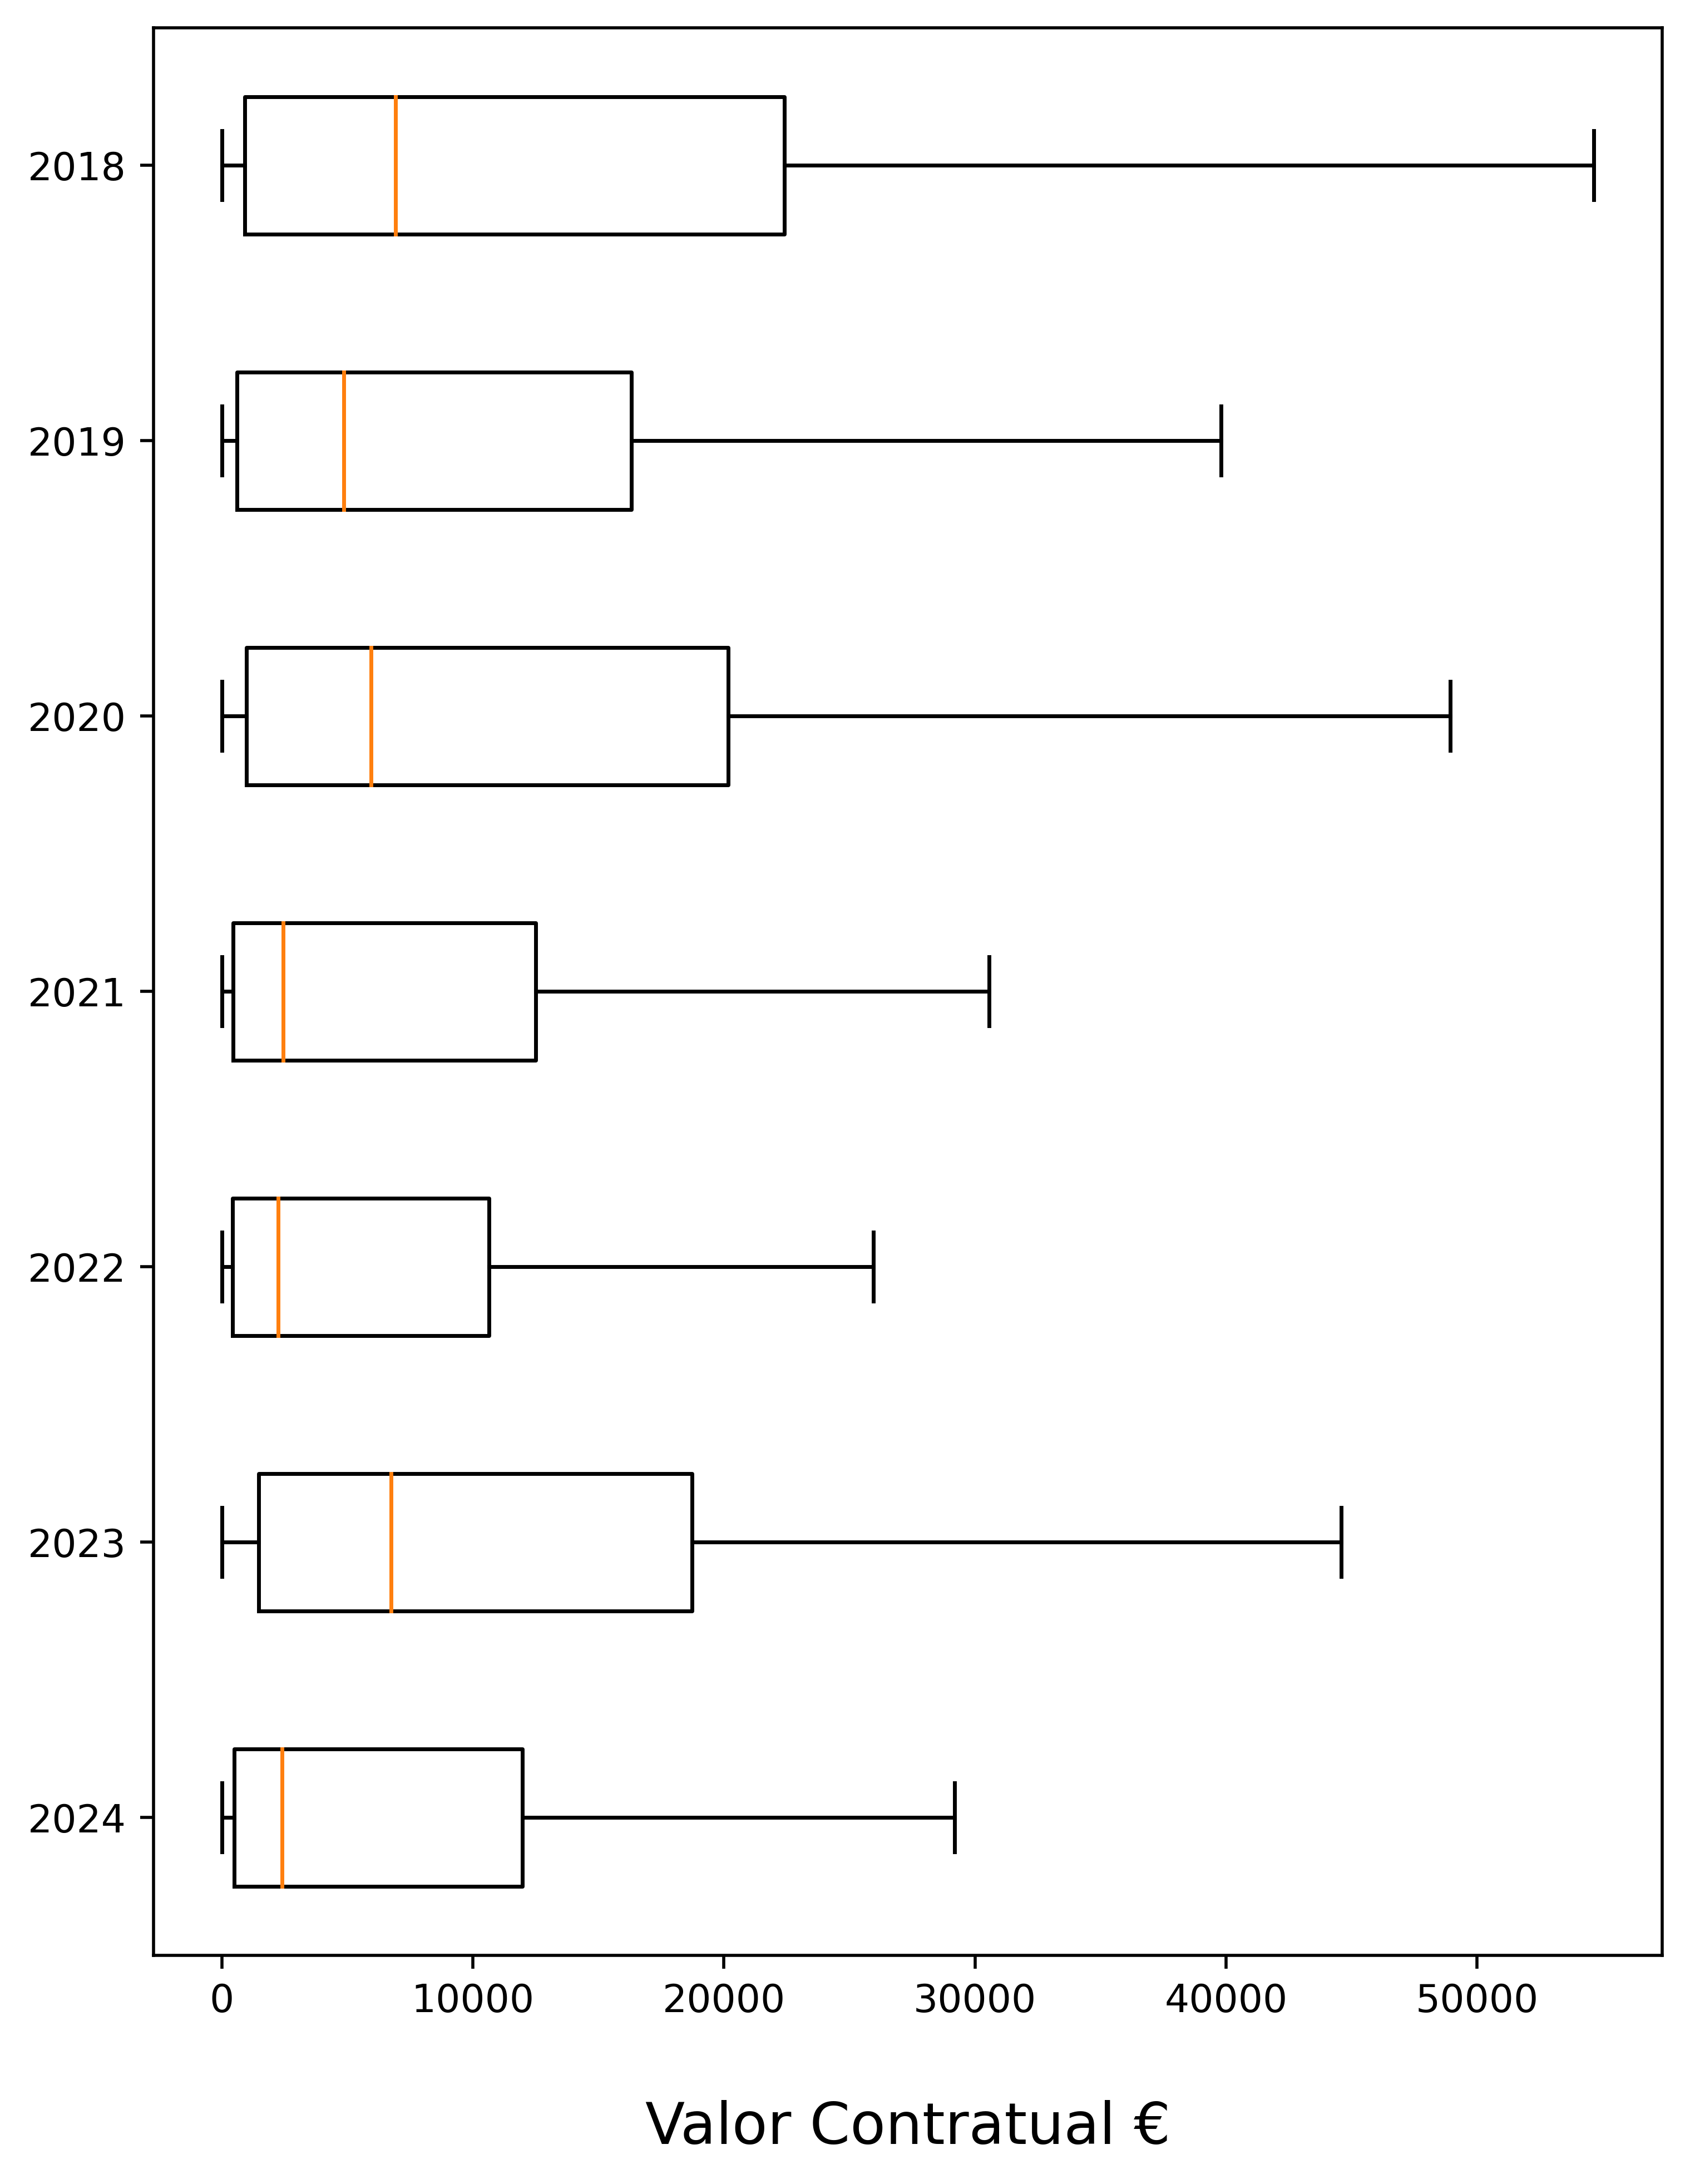
\includegraphics[width=\textwidth]{imagens/ajdir_anos33_v1.png}
%		\caption{Boxplot dos preços contratuais para ajustes diretos em regime geral referentes à área da saúde desde 2018 até 2024}
%	\end{minipage}%
%	\hfill% not: "\hspace{0.5cm}"
%	\begin{minipage}{0.33\linewidth}
%		%\centering  % redundant
%		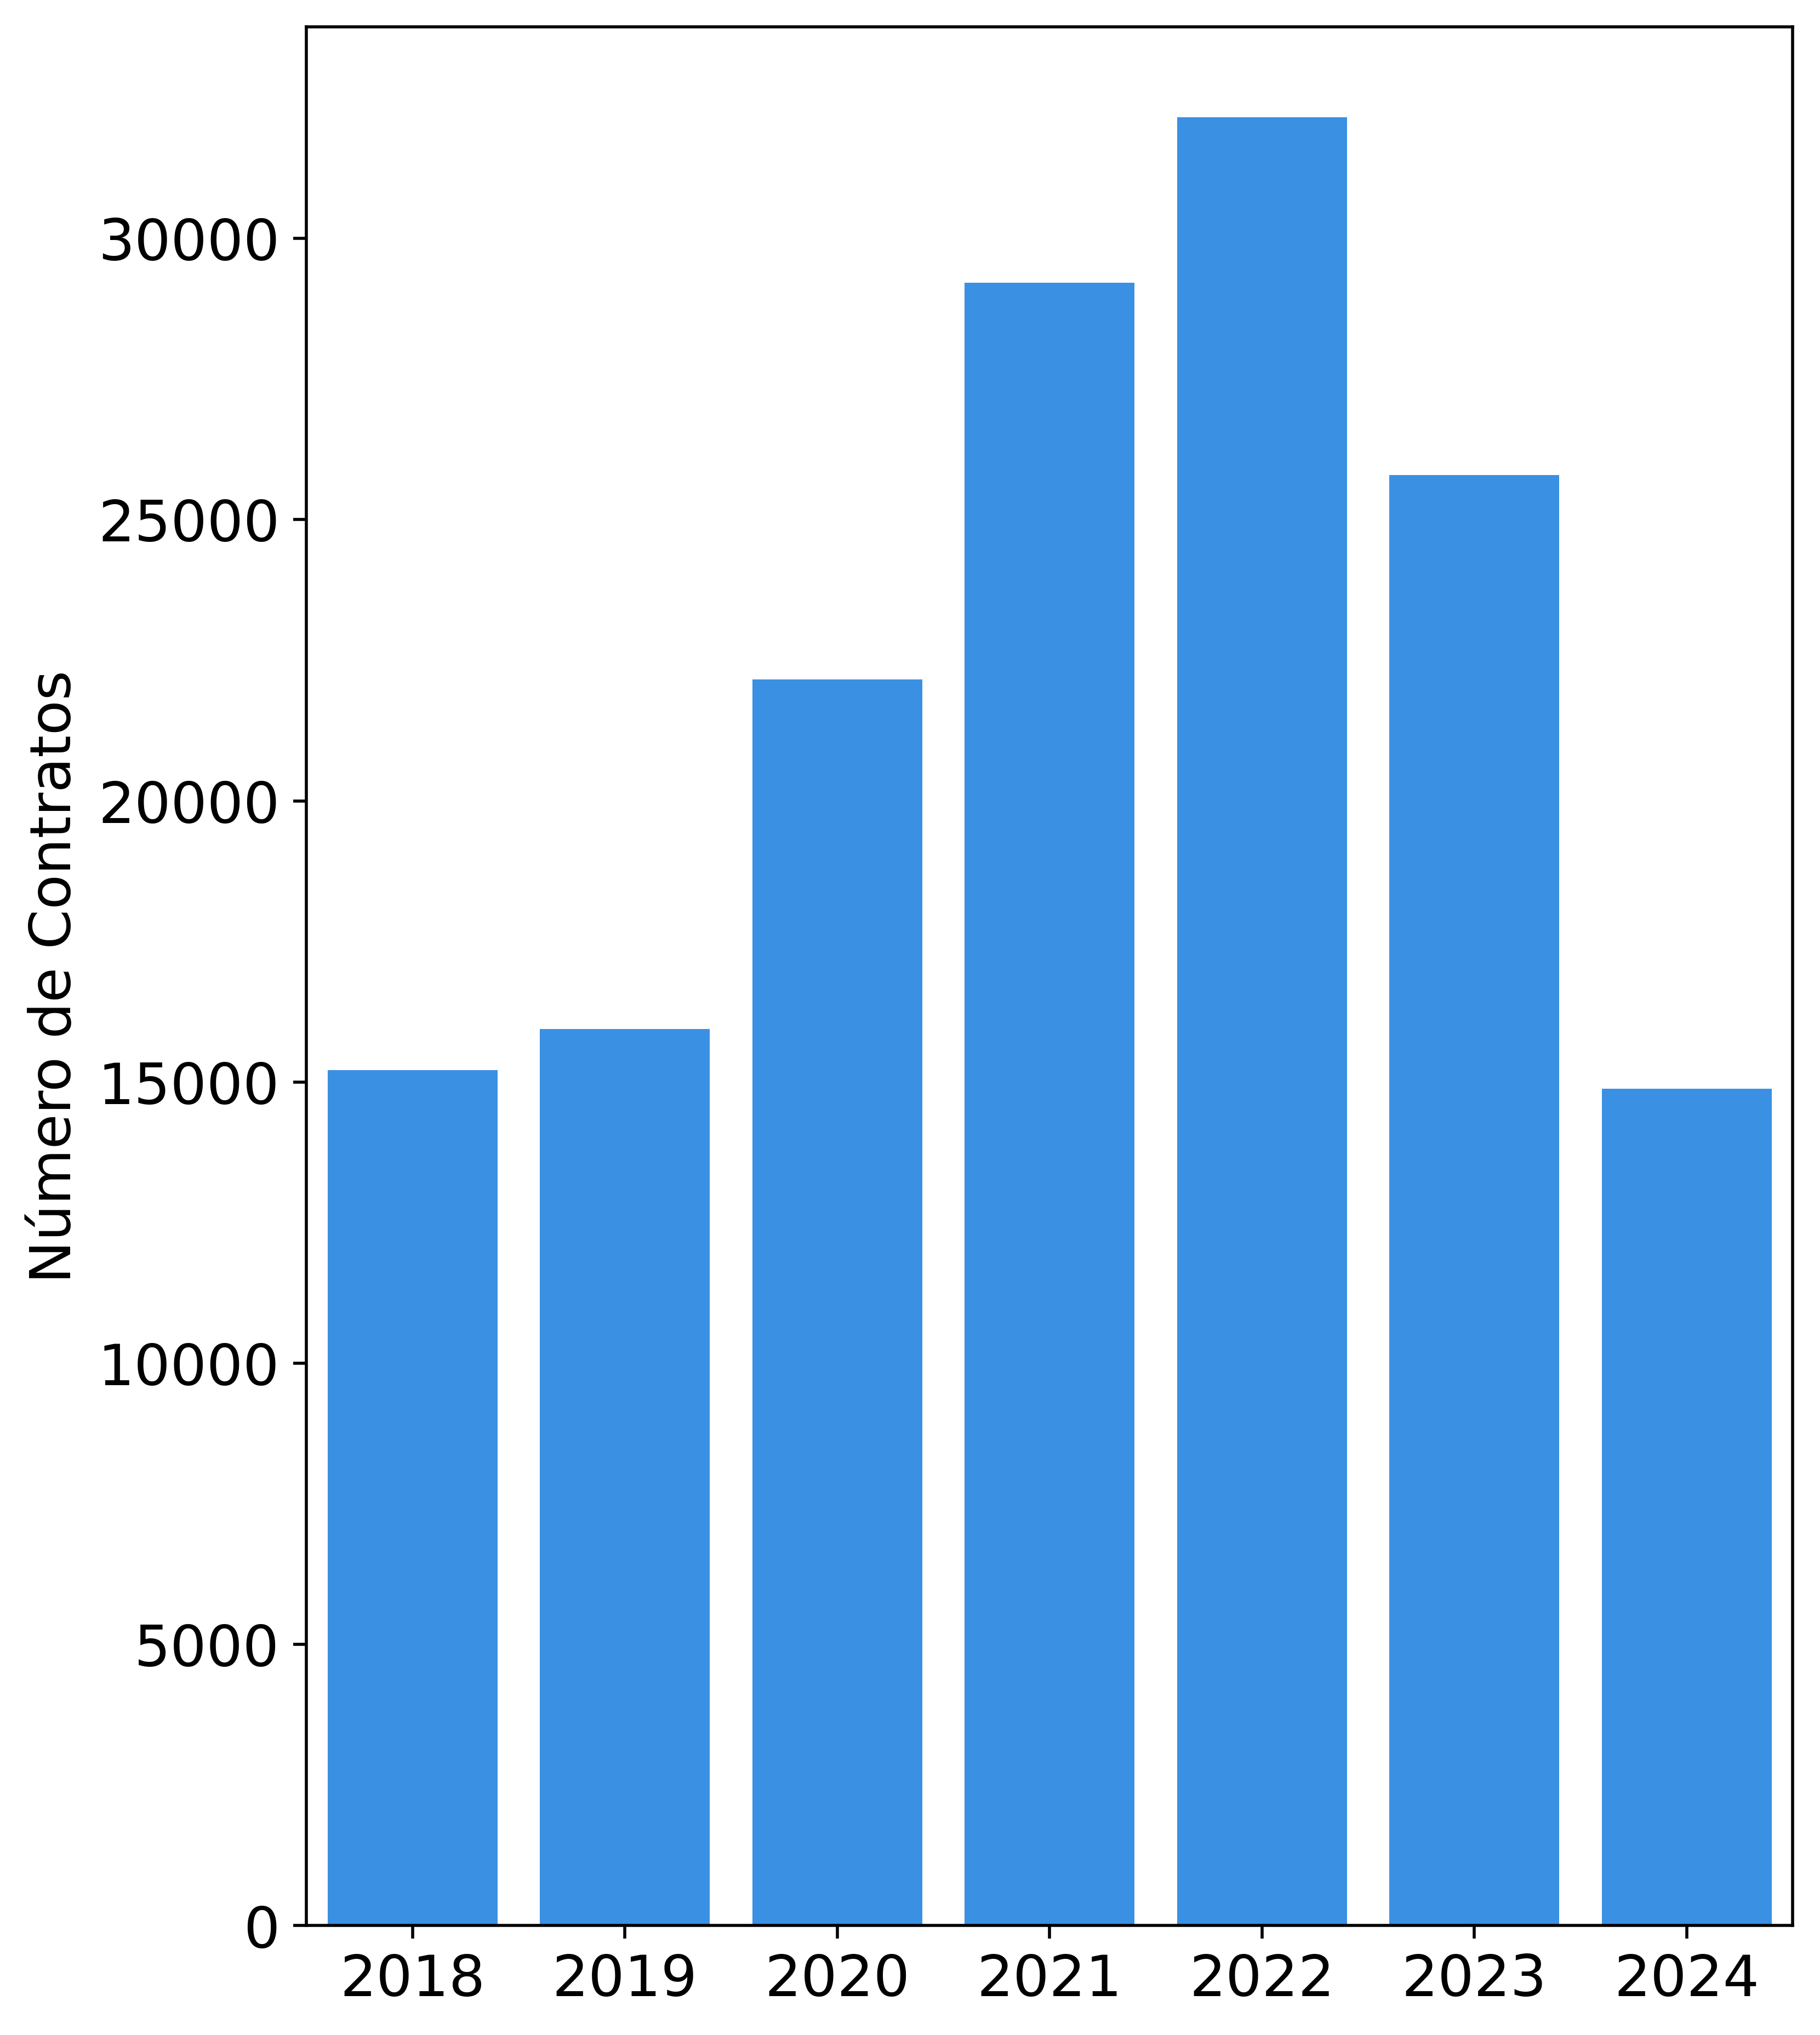
\includegraphics[width=\textwidth]{imagens/ajdir_anos33_v2.png}
%		\caption{Número de ajustes diretos em regime geral celebrados referentes à área da saúde desde 2018 até 2024}
%	\end{minipage}%
%	\hfill% not: "\hspace{0.5cm}"
%	\begin{minipage}{0.33\linewidth}
%		%\centering  % redundant
%		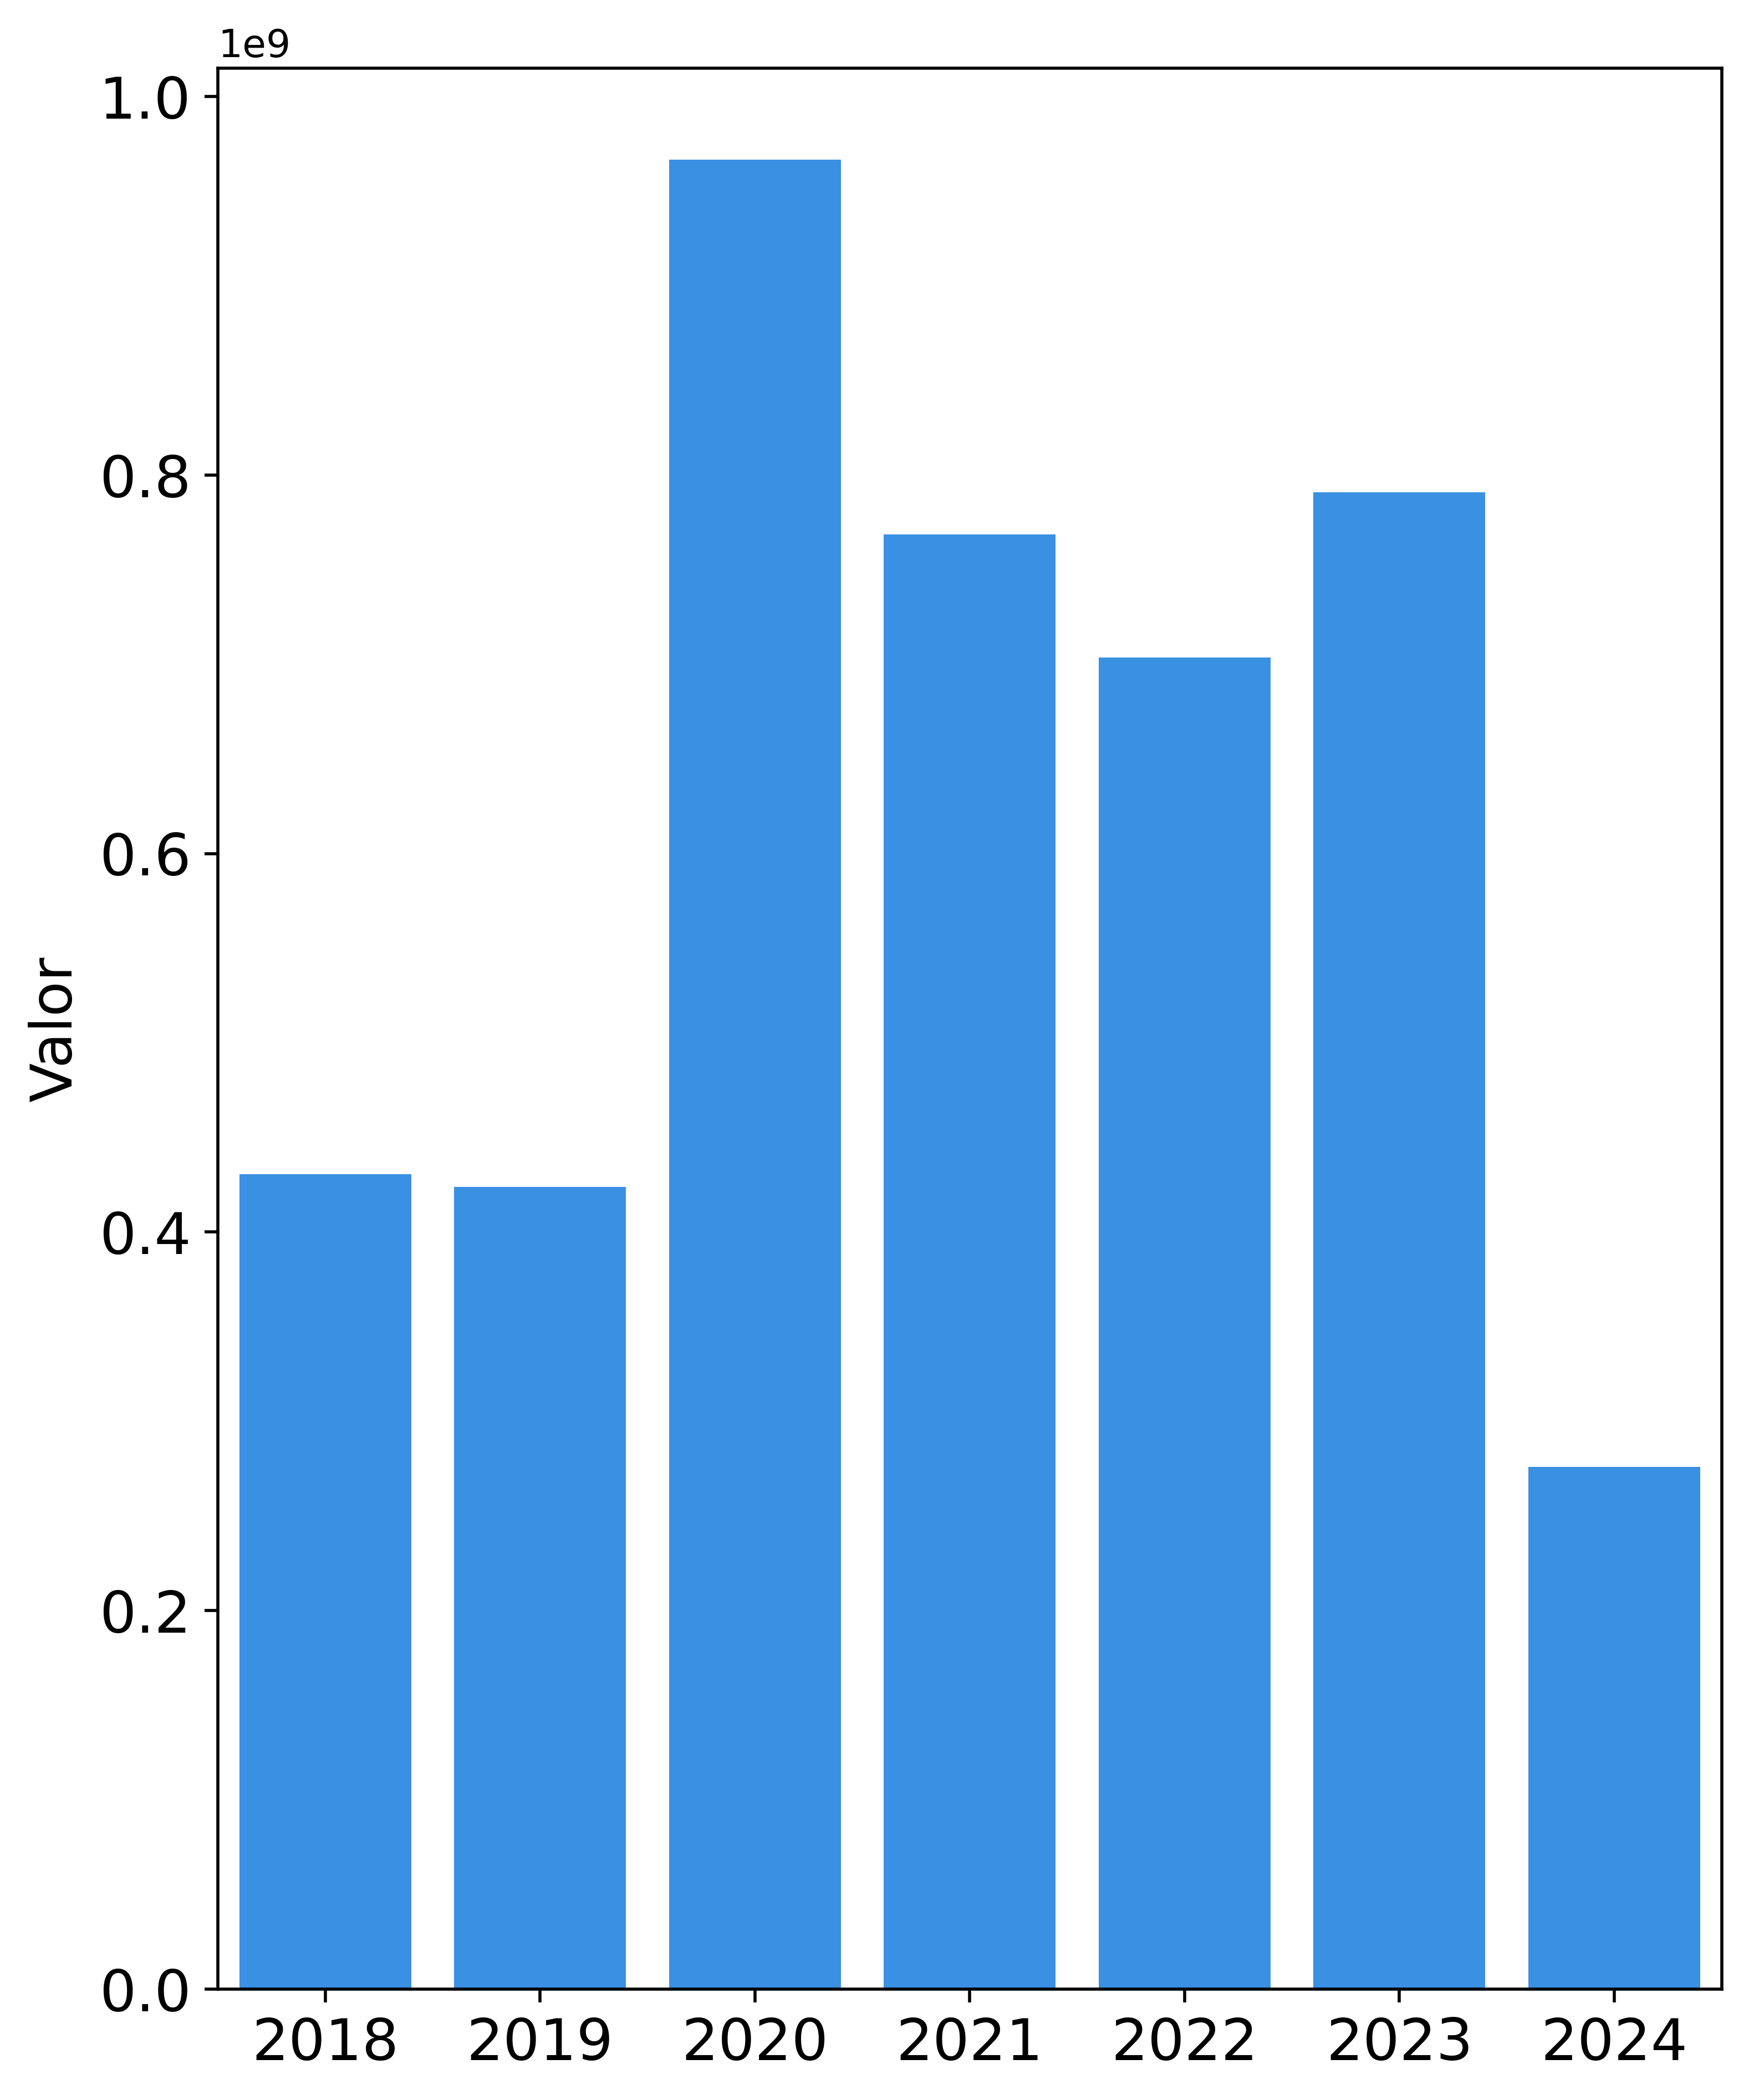
\includegraphics[width=\textwidth]{imagens/ajdir_anos33_v3.png}
%		\caption{Montante total adjudicada a ajustes diretos em regime geral celebrados referentes à área da saúde desde 2018 até 2024}
%	\end{minipage}
%\end{figure}

















